\documentclass[12pt,a4paper,twoside,openright]{book}

% --- LINGUA E CODIFICA ---
\usepackage[utf8]{inputenc}
\usepackage[T1]{fontenc}
\usepackage[english]{babel}
\usepackage{lmodern}


% --- PROFONDITA' INDICE E NUMERAZIONE ---
%\setcounter{secnumdepth}{3} % Numera fino alle subsubsection (es. 1.1.1.1)
%\setcounter{tocdepth}{3}% Mostra le subsubsection nell'indice

% --- PROFONDITA' INDICE E NUMERAZIONE ---
\setcounter{secnumdepth}{3} % Mantiene i numeri nel testo per le subsubsection (es. 1.1.1.1)
\setcounter{tocdepth}{2}% L'indice si ferma alle subsection (es. 1.1.1), nascondendo i livelli inferiori

% --- LAYOUT E GEOMETRIA ---
\usepackage{geometry}
\geometry{
a4paper,
top=3cm,% Aumentato per dare respiro alla testata
bottom=3cm, % Aumentato per dare respiro al numero di pagina
left=2.5cm,
right=2.5cm,
heightrounded,
bindingoffset=5mm, % FONDAMENTALE per la rilegatura
includehead,
includefoot
}

% --- BIBLIOGRAFIA ---
\usepackage[backend=biber, style=numeric, sorting=none]{biblatex}
\addbibresource{biblio.bib} % Collega il file che hai appena creato

% Importazione del tuo file di stile modificato (copertina, ecc.)
\usepackage{style/isi-lt}

% --- MATEMATICA E SIMBOLI ---
\usepackage{amsmath}
\usepackage{amssymb}
\usepackage{amsthm}
\usepackage{amsfonts}
\usepackage{bm} % Per il grassetto nelle formule matematiche

% --- GRAFICA E COLORI ---
\usepackage{graphicx}
\usepackage[dvipsnames]{xcolor}
\usepackage{tikz}
\usetikzlibrary{positioning, arrows.meta, shapes.geometric, calc} 

% --- TABELLE ---
\usepackage{booktabs}
\usepackage{longtable}
\usepackage{tabularx}
\usepackage{array}

% --- ALGORITMI ---
\usepackage{algorithm}
\usepackage{algpseudocode}
% Traduzione delle keywords degli algoritmi
\algnewcommand\Inputs{\item[\textbf{Input:}]}
\algnewcommand\Outputs{\item[\textbf{Output:}]}
\algnewcommand\Initialization{\item[\textbf{Initialization:}]}

% --- LISTE ED ENUMERAZIONI ---
\usepackage{enumitem}

% --- INTESTAZIONI E PIÈ DI PAGINA ---
\usepackage{fancyhdr}
\setlength{\headheight}{27.11652pt}
\addtolength{\topmargin}{-12.61652pt}
\pagestyle{fancy}
\fancyhf{}
\fancyhead[L]{\leftmark}
\fancyfoot[C]{\thepage}

% Reduce minor overfull boxes in paragraphs (allows a tiny amount of stretch)
\usepackage[final]{microtype}

% Avoid underfull vbox warnings by allowing pages to stretch slightly (common with book class / floats)
\raggedbottom

% Avoid underfull vbox warnings by allowing pages to stretch slightly (common with book class / floats)
\raggedbottom

% --- CROSS-REFERENCING (Sempre per ultimo o quasi) ---
\usepackage{hyperref}
\hypersetup{
colorlinks=true,
linkcolor=black,
filecolor=magenta,
urlcolor=Blue,
pdftitle={Thesis Title - Riccardo Balzani}, % Suggerisco di mettere il titolo o il tuo nome
pdfpagemode=FullScreen,
}
\usepackage[all]{hypcap} % Per far sì che i link alle figure puntino all'immagine e non alla didascalia

% --- DEFINIZIONE AMBIENTI TEORICI---
\newtheorem{theorem}{Theorem}[chapter]
\newtheorem{definition}{Definition}[chapter]
\newtheorem{lemma}{Lemma}[chapter]
\newtheorem{proposition}{Proposition}[chapter]
\newtheorem{corollary}{Corollary}[chapter]

\usepackage[skins]{tcolorbox}
\newtcolorbox{promptbox}{
enhanced,
boxrule=0pt, % Removes top, right, and bottom borders
leftrule=3pt,% Creates the thick left border
arc=2.5mm, % Sets the roundness of the corners
colframe=blue!60!black,% Color of the left border
colback=blue!10!white,% Color of the background
fontupper=\itshape
}


% --- AMBIENTE PER CODICE PYTHON ---
% --- AMBIENTE PER CODICE PYTHON (COLORI AVANZATI) ---
\usepackage{listings}
\tcbuselibrary{listings} 

% Definizione dei colori (Stile VS Code Light)
\definecolor{pykeyword}{HTML}{0000FF}   % Blu per parole chiave (def, return, and, if...)
\definecolor{pystring}{HTML}{A31515}    % Rosso scuro per stringhe e docstring
\definecolor{pycomment}{HTML}{008000}   % Verde per i commenti
\definecolor{pytype}{HTML}{2B91AF}      % Teal/Azzurro per i tipi (str, int, Tuple...)
\definecolor{pybuiltin}{HTML}{795E26}   % Senape per funzioni built-in (len, split...)
\definecolor{pybg}{HTML}{F6F8FA}        % Sfondo chiaro stile GitHub (invariato)
\definecolor{pyframe}{HTML}{D0D7DE}     % Bordo grigio chiaro (invariato)

% Definizione del nuovo ambiente "pythoncode"
\newtcblisting{pythoncode}[1][]{
    enhanced,
    arc=3mm,
    boxrule=0.8pt,
    colframe=pyframe,
    colback=pybg,
    drop shadow=gray!20!white,
    boxsep=2pt,
    left=15pt,
    right=4pt,
    top=4pt,
    bottom=4pt,
    title=#1,
    fonttitle=\bfseries\sffamily\small,
    coltitle=black,
    colbacktitle=pybg,
    attach boxed title to top left={xshift=5mm, yshift=-2mm},
    boxed title style={colback=white, colframe=pyframe, boxrule=0.8pt, arc=2mm},
    listing only,
    listing options={
        language=Python,
        basicstyle=\ttfamily\footnotesize\color{black}, % Le variabili standard restano nere
        keywordstyle=\color{pykeyword}\bfseries,
        stringstyle=\color{pystring},
        commentstyle=\color{pycomment}\itshape,
        % --- 1. Gruppo: Tipi di dato ---
        emph={int, str, bool, float, Tuple, List, Dict, Set, Any, Union, Optional},
        emphstyle=\color{pytype},
        % --- 2. Gruppo: Funzioni built-in e metodi comuni ---
        emph={[2]len, print, range, enumerate, split, append, text, ents},
        emphstyle={[2]\color{pybuiltin}},
        numberstyle=\tiny\color{gray},
        numbers=left,
        stepnumber=1,
        numbersep=10pt,
        showstringspaces=false,
        breaklines=true,
        frame=none,
        tabsize=4
    }
}

% TABELLA DEI RISULTATI 

\usepackage{multirow}      % Per unire le righe verticalmente
\usepackage{makecell}      % Per andare a capo dentro le celle e formattazione avanzata
\usepackage{fontawesome5}  % Per l'icona \faEye
\usepackage{colortbl}     % Per colorare le celle (già richiamato in parte da xcolor)
\usepackage{arydshln}     % FONDAMENTALE per \cdashline (linee tratteggiate)

% --- DEFINIZIONE COLORI TABELLA ---
\definecolor{cellhighlight}{HTML}{E7E7E7}    % Grigio chiaro per i risultati migliori
\definecolor{tablehighlight}{HTML}{F5F5F5}   % Sfondo per la legenda
\definecolor{tablebordercolor}{HTML}{666666} % Colore bordi legenda

% --- MACRO PLACEHOLDER PER ICONE/ETICHETTE ---
% Sostituisci i testi con icone o simboli se preferisci
\newcommand{\rawImage}[1][0.15in]{\textit{Img}}
\newcommand{\seg}[1][0.15in]{\textit{Seg}}
\newcommand{\segNumObj}[1][0.15in]{\textit{Seg+ID}}
\newcommand{\gom}{\textbf{GOM}}
\newcommand{\gomLabObj}[1][0.4in]{\textit{G-Lab}}
\newcommand{\gomNumObj}[1][0.4in]{\textit{G-Num}}
\newcommand{\gomLabObjLabRel}[1][0.4in]{\textit{G-LabRel}}
\newcommand{\gomNumObjLabRel}[1][0.4in]{\textit{G-NumRel}}

% --- ICONE PIPELINE (Versione Regular/Light) ---

% 1. Routing / NER
\newcommand{\nerOn}{\faIcon[regular]{filter}}       % Filtro "vuoto"
\newcommand{\nerOff}{\faBan}
\newcommand{\query}{\faIcon[regular]{file-alt}}    % Documento con righe (richiesto dal tutor)

% 2. Preprocessing Types
\newcommand{\typeRaw}{\faIcon[regular]{image}}      % Icona immagine outline
\newcommand{\typeAttn}{\faIcon{crosshairs}}         % Mirino (già leggero di suo)
\newcommand{\typeBBox}{\faIcon{vector-square}}      % Bounding Box (già outline)
\newcommand{\typeSeg}{\faIcon[regular]{puzzle-piece}} % Pezzo di puzzle outline

\newcommand{\iconEye}{\faIcon[regular]{eye}}

\newcommand{\iconEval}{\faBalanceScale}

% Colore leggero per l'eccellenza
\definecolor{bestcolor}{gray}{0.9} % Un grigio molto chiaro


% 3. Macro per combinare i due step nella cella
% Uso: \pipe{NER_CMD}{TYPE_CMD} -> es. \pipe{\nerOn}{\typeSeg}
\newcommand{\pipe}[2]{#1\,$\to$\,#2}

% Macro per semplificare la riga della tabella
% Uso: \pipeline{Icona1}{Icona2}
\newcommand{\pipeline}[2]{#1\pipeArrow #2}

%%%%%%%%%%%%%%%%%%%%%%%%%%%%%%%%%%%%%%%%%%
%Copertina %
%%%%%%%%%%%%%%%%%%%%%%%%%%%%%%%%%%%%%%%%%%%%%%

\campus{Cesena Campus}
\dipartimento{Department of Computer Science and Engineering}
\cdl{Bachelor's Degree in Computer Science and Engineering}

\titolo{Visual Grounding in Medical Question Answering: Evaluating the Impact of Image Prompting on Multimodal Large Language Models}

\laureando{Balzani Riccardo}

\relatore[Prof.]{Moro Gianluca}
\correlatoreA[Dr.]{Molfetta Lorenzo}
\correlatoreB[Dr.]{Fantazzini Stefano}

\annoaccademico{2024 -- 2025}

\materia{DATA INTENSIVE APPLICATIONS}

\dedica{
''\emph{Tutto è} \textbf{Possibile}''

\vspace{0.5em}

\hspace*{\fill}--- Boh ???
}

\makeindex


\DeclareUnicodeCharacter{2212}{-}
%%%%%%%%%%%%%%%%%%%%%%%%%%%%%%%%%%%%%%%%%%%%%%
% Inizio Documento %
%%%%%%%%%%%%%%%%%%%%%%%%%%%%%%%%%%%%%%%%%%%%%%

\begin{document}

\pagestyle{plain}

\maketitle

\frontmatter % Numeri della pagina ROMANI
\pagenumbering{Roman}

\tableofcontents

\pagestyle{fancy}

%%%%%%%%%%%%%%%%%%%%%%%%%%%%%%%%%%%%%%%%%%%%%%
% Introduzione %
%%%%%%%%%%%%%%%%%%%%%%%%%%%%%%%%%%%%%%%%%%%%%%
\input{parts/introduction.tex}


\mainmatter %Numeri della pagina ARABI

%%%%%%%%%%%%%%%%%%%%%%%%%%%%%%%%%%%%%%%%%%%%%%
% CAPITOLO 1                                 %
%%%%%%%%%%%%%%%%%%%%%%%%%%%%%%%%%%%%%%%%%%%%%%
\chapter{Theoretical Framework}
The processing of sequential data constitutes a foundational pillar of modern Artificial Intelligence, particularly in Natural Language Processing (NLP) and, by extension, multimodal applications. For years, the state of the art in sequence modeling was defined by recurrent architectures \cite{rnn_sequence}, which, despite their successes, presented structural limitations regarding scalability and the retention of long-range dependencies \cite{analyticsvidhya}. The advent of the Transformer architecture marked a paradigm shift in the field, overcoming these bottlenecks through the introduction of the self-attention mechanism \cite{arxiv-attention}.\par
This chapter traces this crucial architectural evolution. The first section examines the theoretical foundations, operational mechanics, and inherent limitations of Recurrent Neural Networks (RNNs). Building upon this context, the subsequent sections delve into the Transformer architecture, detailing its core components and explaining how its highly parallelizable nature established the groundwork for modern Large Language Models (LLMs).

\section{Recurrent Neural Networks: Pre-Transformer State of the Art}
\label{chap:rnn}
\noindent
In recent years, the field of Artificial Intelligence has experienced an extraordinary evolution, driven by advances in deep learning, the increase in GPU computational power, and the availability of large-scale data. Until 2017, the majority of models for processing sequential data—such as text, biomedical signals, and time series—relied on \textbf{Recurrent Neural Networks (RNNs)} \cite{rnn_sequence, cs231n-rnn, quarkml-rnn-explained} and their variants, including Long Short-Term Memory (LSTM) networks, introduced by Hochreiter and Schmidhuber (1997), and Gated Recurrent Units (GRUs). These models represented the state of the art due to their ability to capture temporal dependencies and maintain memory of previous states, finding applications in speech recognition, machine translation, and natural language processing.

Although gating mechanisms mitigated the \textbf{vanishing/exploding gradient} problem \cite{quarkml-bptt}, recurrent architectures presented substantial limitations: \textbf{strictly sequential processing} hindered efficient parallelization, slowing down training on large datasets, and \textbf{modeling long-range dependencies} remained difficult, even when employing bidirectional variants or regularization strategies \cite{analyticsvidhya}. The breakthrough came in 2017 with the Transformer architecture, which replaced recurrence with \textbf{self-attention} mechanisms, allowing for the parallel processing of all positions in a sequence and more effective modeling of long-range relationships.

With the aim of contextualizing the advent of Transformers, this first section clearly introduces the basic operation of RNNs, highlighting their principles, strengths, and main limitations, thus laying the groundwork for comparison with subsequent architectures.

\subsection{RNN Architecture Overview}
\label{sub:recurrent_neural_networks}
\noindent
The distinctive element of \textbf{Recurrent Neural Networks (RNNs)} lies in their recurrent architecture, which allows information to propagate through feedback connections within the network \cite{cs231n-rnn, quarkml-rnn-explained, medium_math_rnn}. Unlike \textbf{Feedforward} neural networks, where data flows unidirectionally from input to output, RNNs introduce lateral connections that allow for the maintenance of temporal information \cite{medium_math_rnn}.

\begin{figure}[H]
\centering
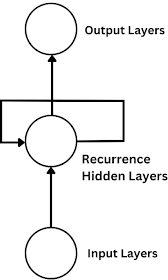
\includegraphics[width=0.25\linewidth]{img/rolled_rnn.png}
\caption{Basic scheme of a Recurrent Neural Network.}
\label{fig:rolled_rnn}
\end{figure}

Ideally, a Recurrent Neural Network can be visualized as a set of \textbf{Feed Forward Neural Networks (FFNNs)} where the hidden layers are connected one-to-one \cite{quarkml-rnn-explained}.
This structure can be understood by imagining a simple FFNN composed of:
\begin{itemize}
\item An input layer
\item Two hidden layers
\item An output layer
\end{itemize}
By connecting each hidden layer to every hidden layer of a second FFNN (constructed in the same way as the previous one) and repeating this operation $N$ times, a model like the one in the figure below is obtained \cite{quarkml-rnn-explained}.

\begin{figure}[H]
\centering
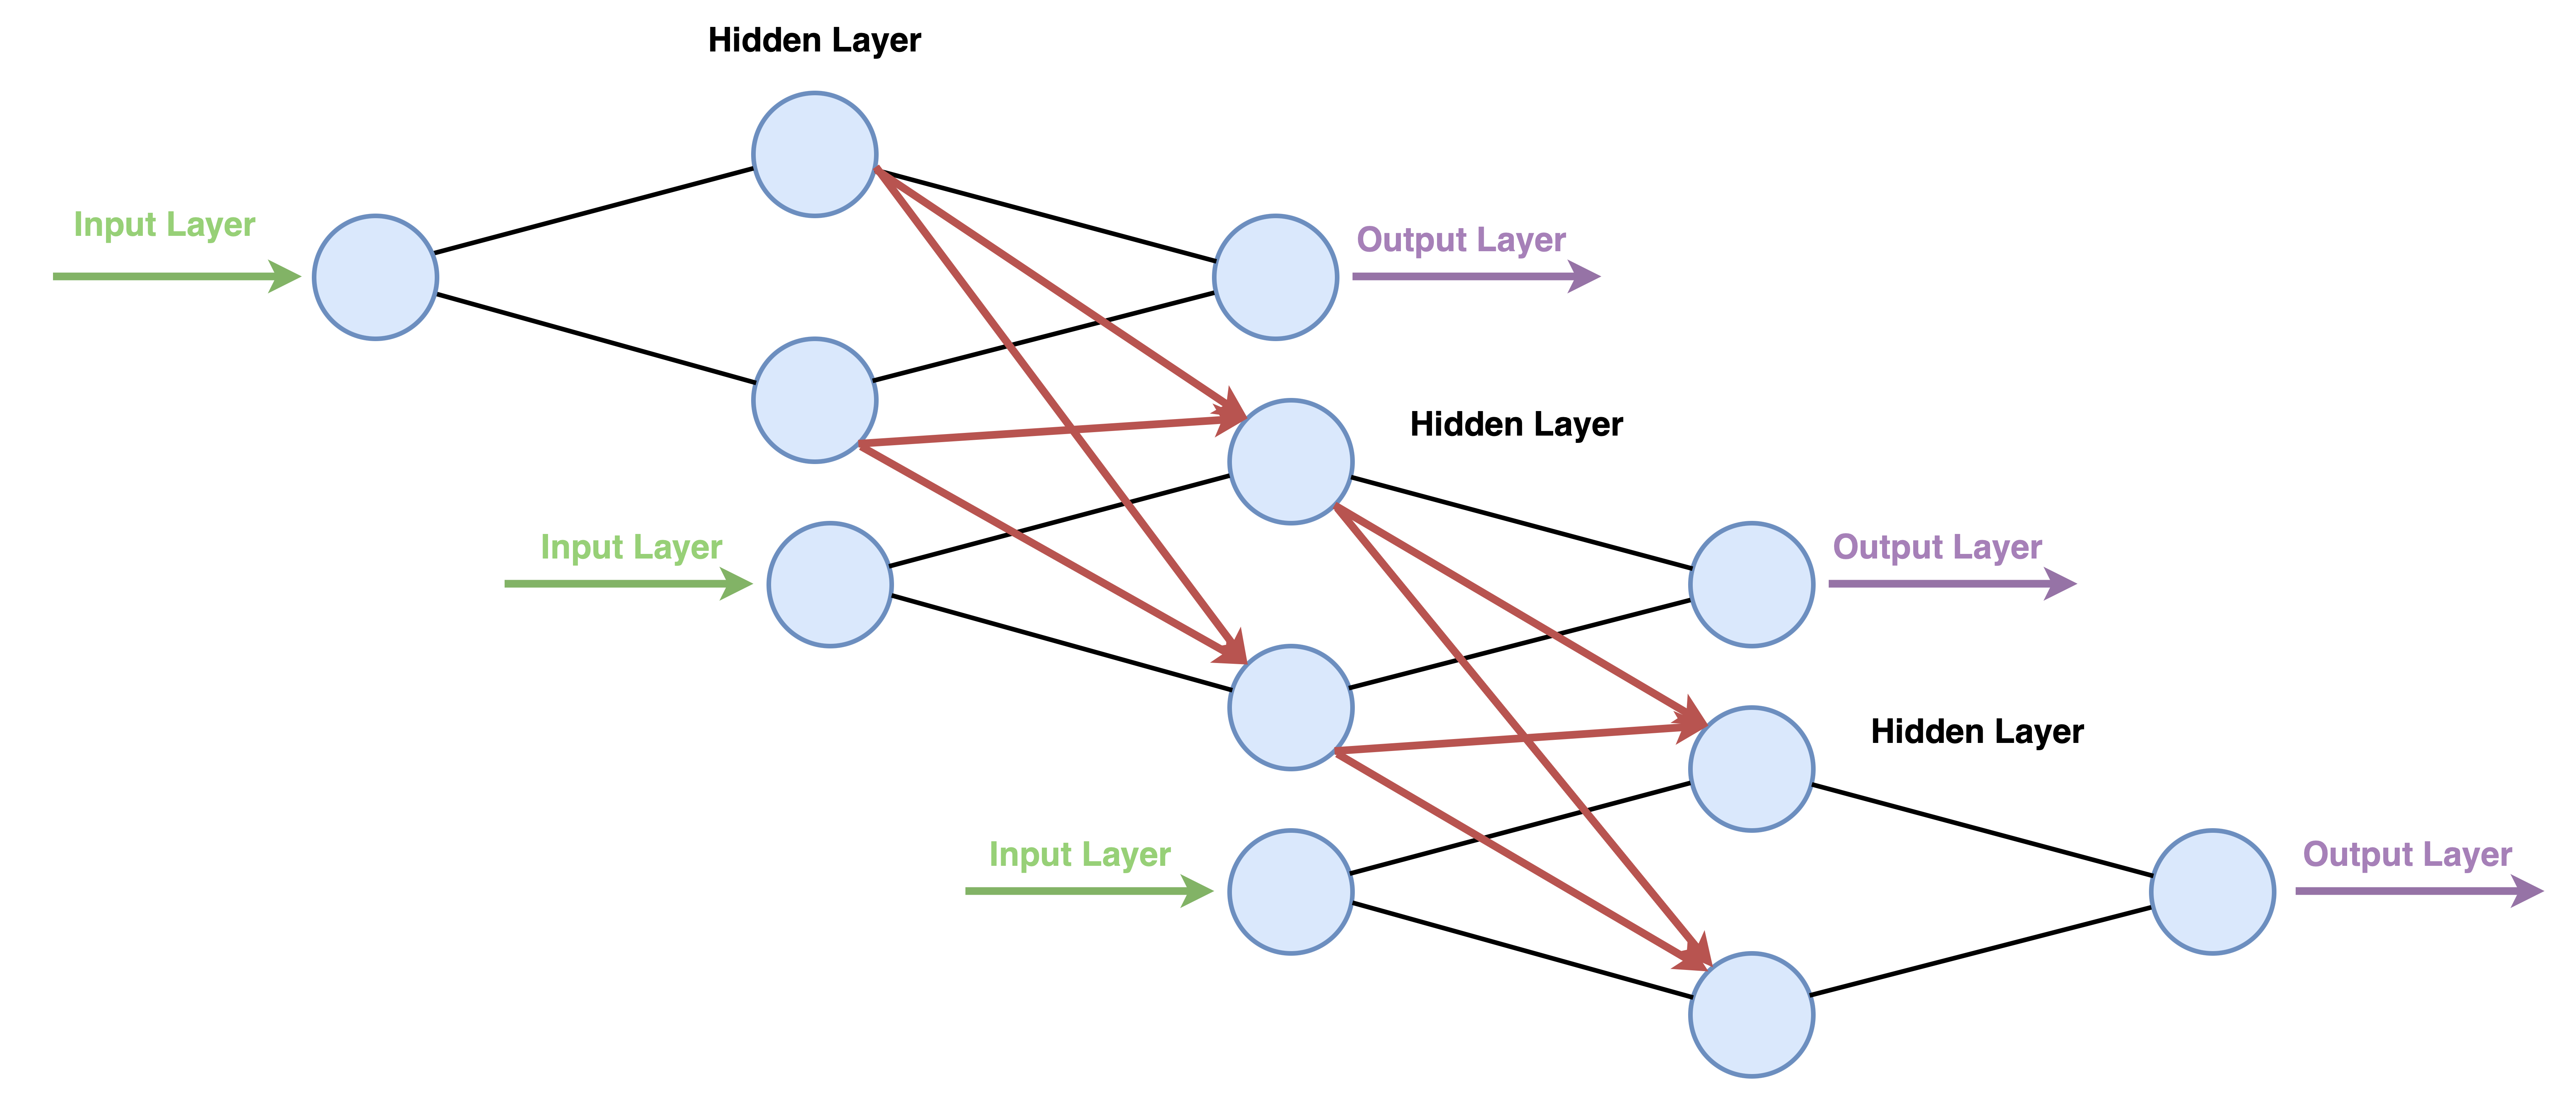
\includegraphics[width=1\linewidth]{img/rnn_hidden_layer2.png}
\caption{Visualization of an RNN with connected hidden layers \cite{quarkml-rnn-explained}. In this case, $N=3$.}
\label{fig:rnn_hidden_layer}
\end{figure}

From Figure \ref{fig:rnn_hidden_layer}, we can therefore understand how the network output depends on both the input from the input layer and the inputs arriving from the recurrent hidden layer.
Each of these individual FFNNs, to which the hidden layers are connected, is called a \textbf{time step} \cite{quarkml-rnn-explained}.

\begin{figure}[H]
\centering
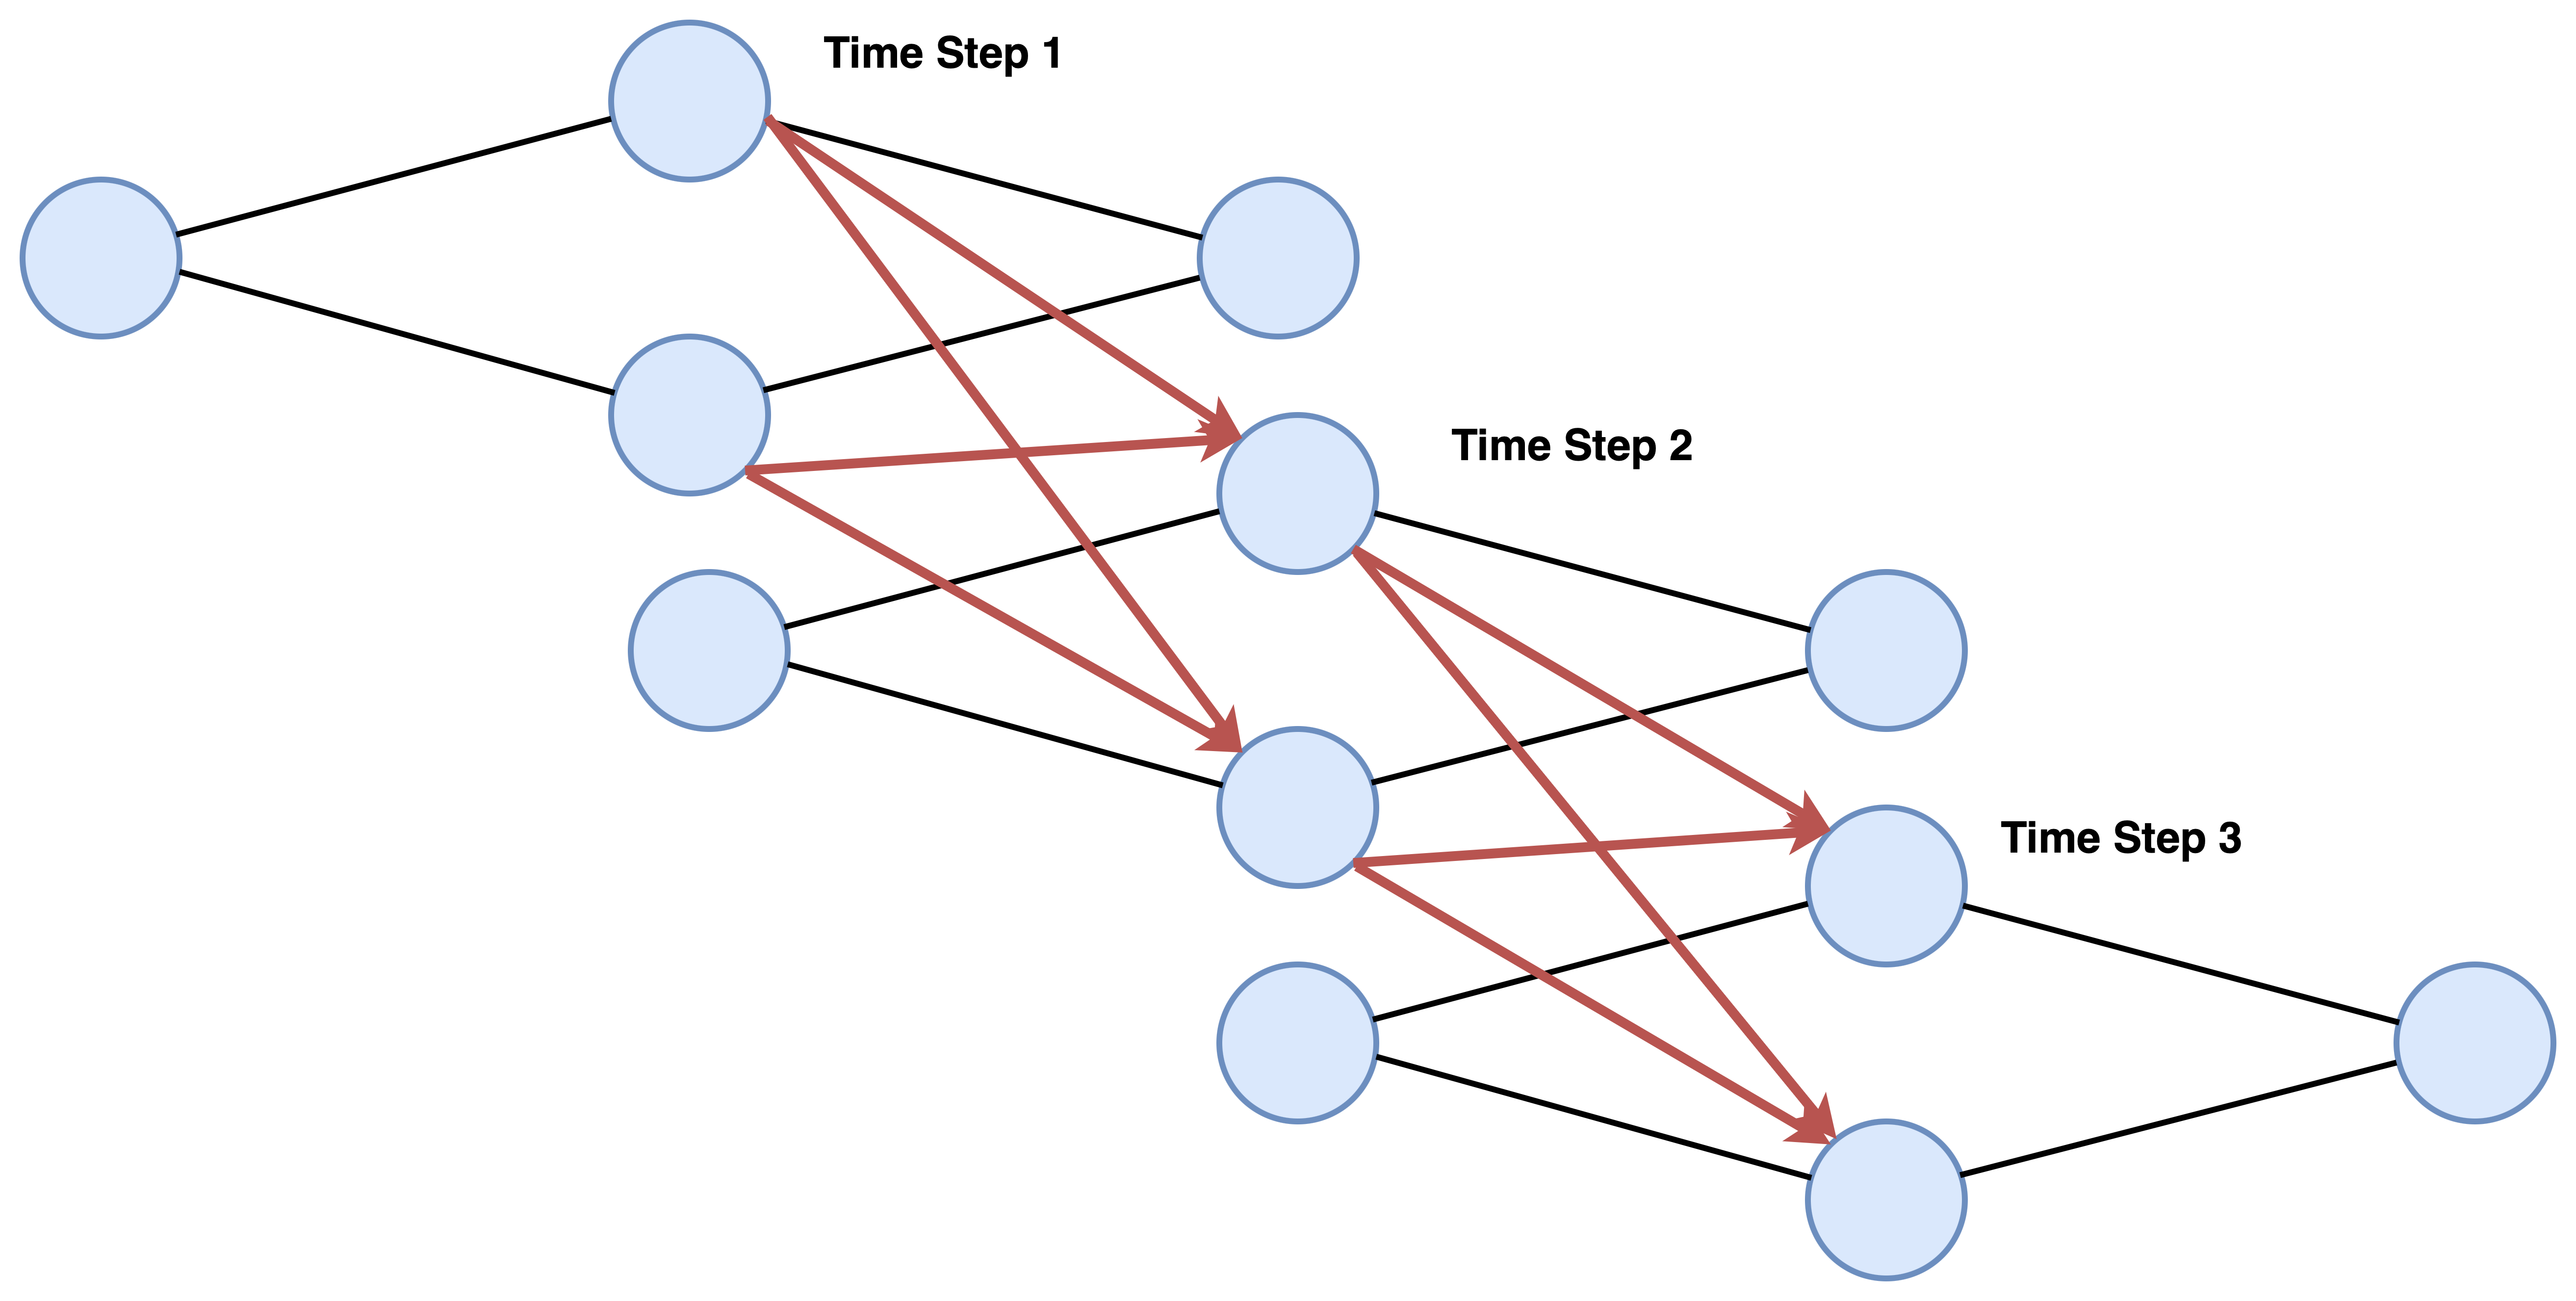
\includegraphics[width=0.8\linewidth]{img/rnn_hidden.png}
\caption{Visualization of an RNN time step \cite{quarkml-rnn-explained}.}
\end{figure}

A time step represents a discrete unit of time in the processing of a data sequence. More precisely, within an RNN, for an input sequence of length $T$, each time step $t$ (where $t$ ranges from $1$ to $T$) corresponds to a specific element of that sequence \cite{quarkml-rnn-explained}.

% spiegazione più concreta RNN.
\subsubsection{Introduction to the Structure of an RNN}
Structurally, an RNN is composed of four fundamental elements \cite{medium_math_rnn, quarkml-rnn-explained}:
\begin{itemize}
\item \textbf{Weights} ($W$): learned matrices that determine the importance of inputs and the previous state in generating the new state.
\item \textbf{Bias} ($b$): vectors added to each calculation to refine the network's response.
\item \textbf{Activation Function}: a \textbf{non-linear} function (e.g., $\tanh$, $\mathrm{ReLU}$, $\sigma$) used to compress the output to manageable values, introducing the capacity to learn complex relationships.
\item \textbf{Feedback Loop}: a recurrent connection that transmits part of the output of one step to the next, allowing the network to maintain a memory of previous information.
\end{itemize}

\begin{figure}[H]
\centering
 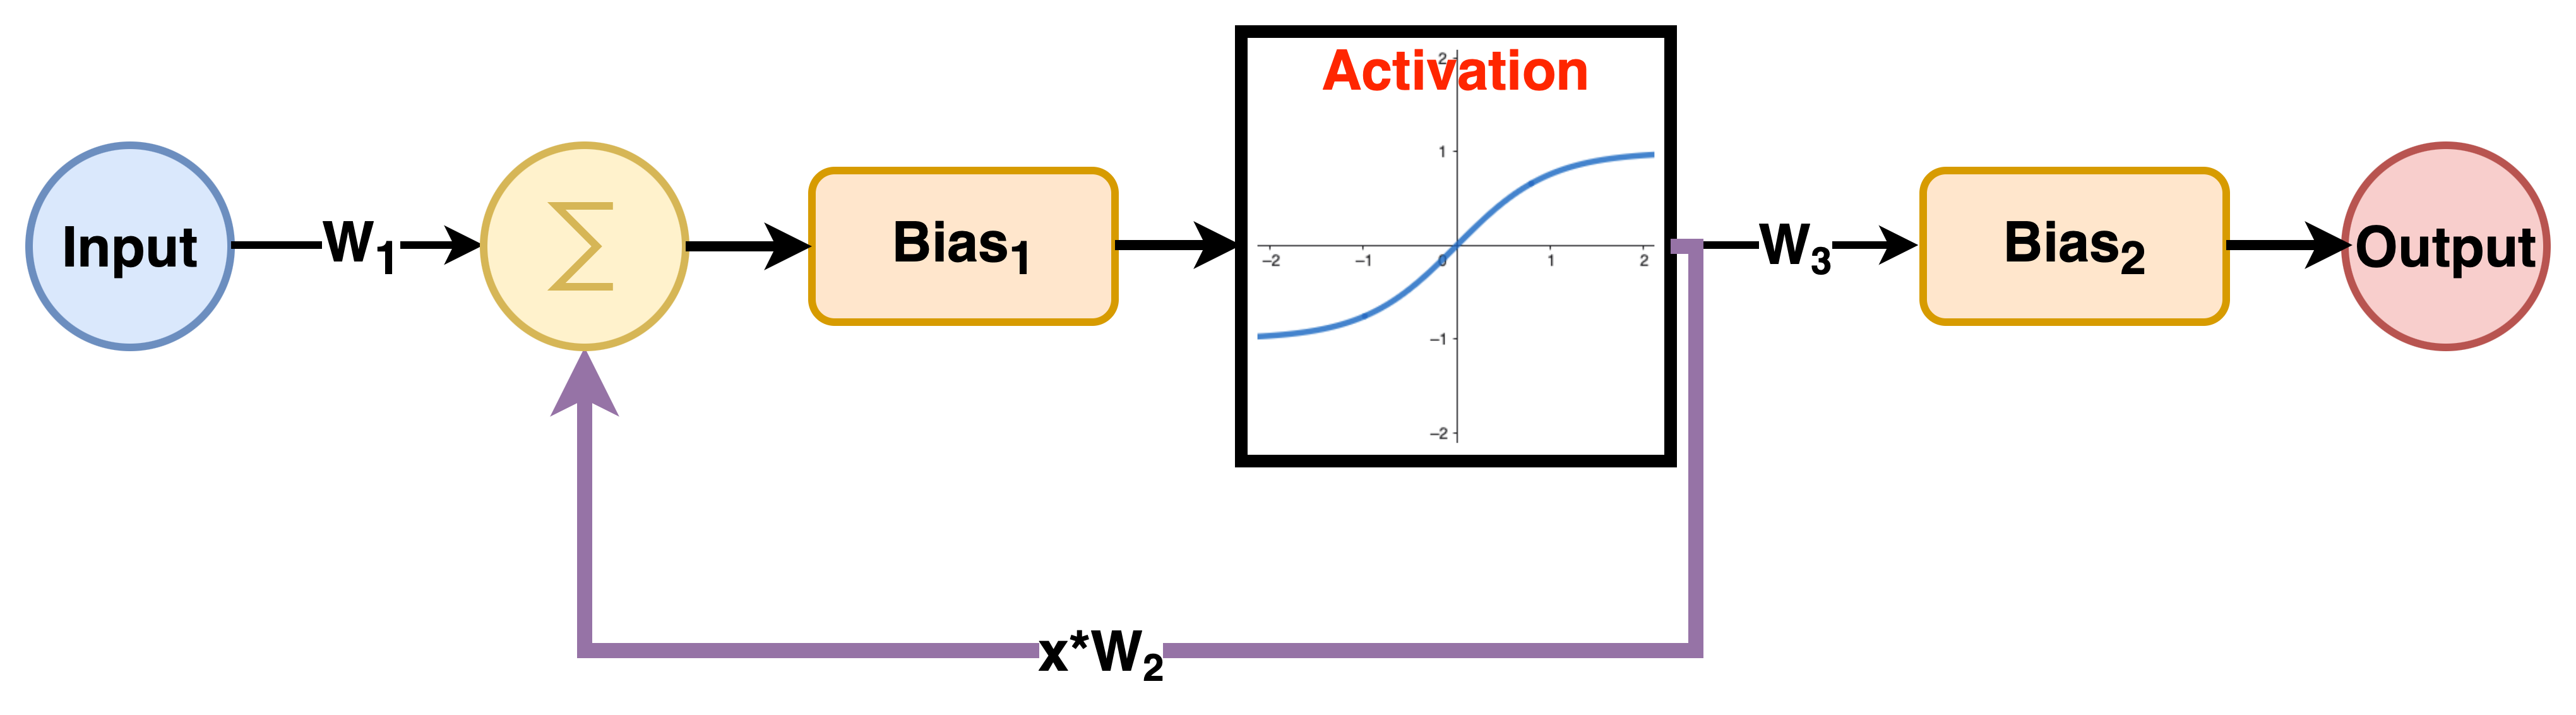
\includegraphics[width=0.8\linewidth]{img/rnn_rolled.png}
 \caption{Structure of an RNN.}
 \label{fig:rnn_rolled}
\end{figure}

The inputs of an RNN consist of a sequence $(input_1, input_2, \ldots, input_T)$, where each element $input_t$ is processed individually at each time step $t$. The \textbf{feedback loop} (highlighted in purple in Figures \ref{fig:rnn_rolled} and \ref{fig:rnn_unrolled}) allows the prediction related to input $input_t$ to be made by leveraging the state generated in the previous step (hidden state $h_{t-1}$) \cite{medium_math_rnn, quarkml-rnn-explained}.
To visualize the operation of an RNN more clearly, it is useful to consider its ``unrolled'' version, known as an \textbf{unrolled RNN}, as shown in Figure \ref{fig:rnn_unrolled} \cite{cs231n-rnn}.

\begin{figure}[H]
\centering
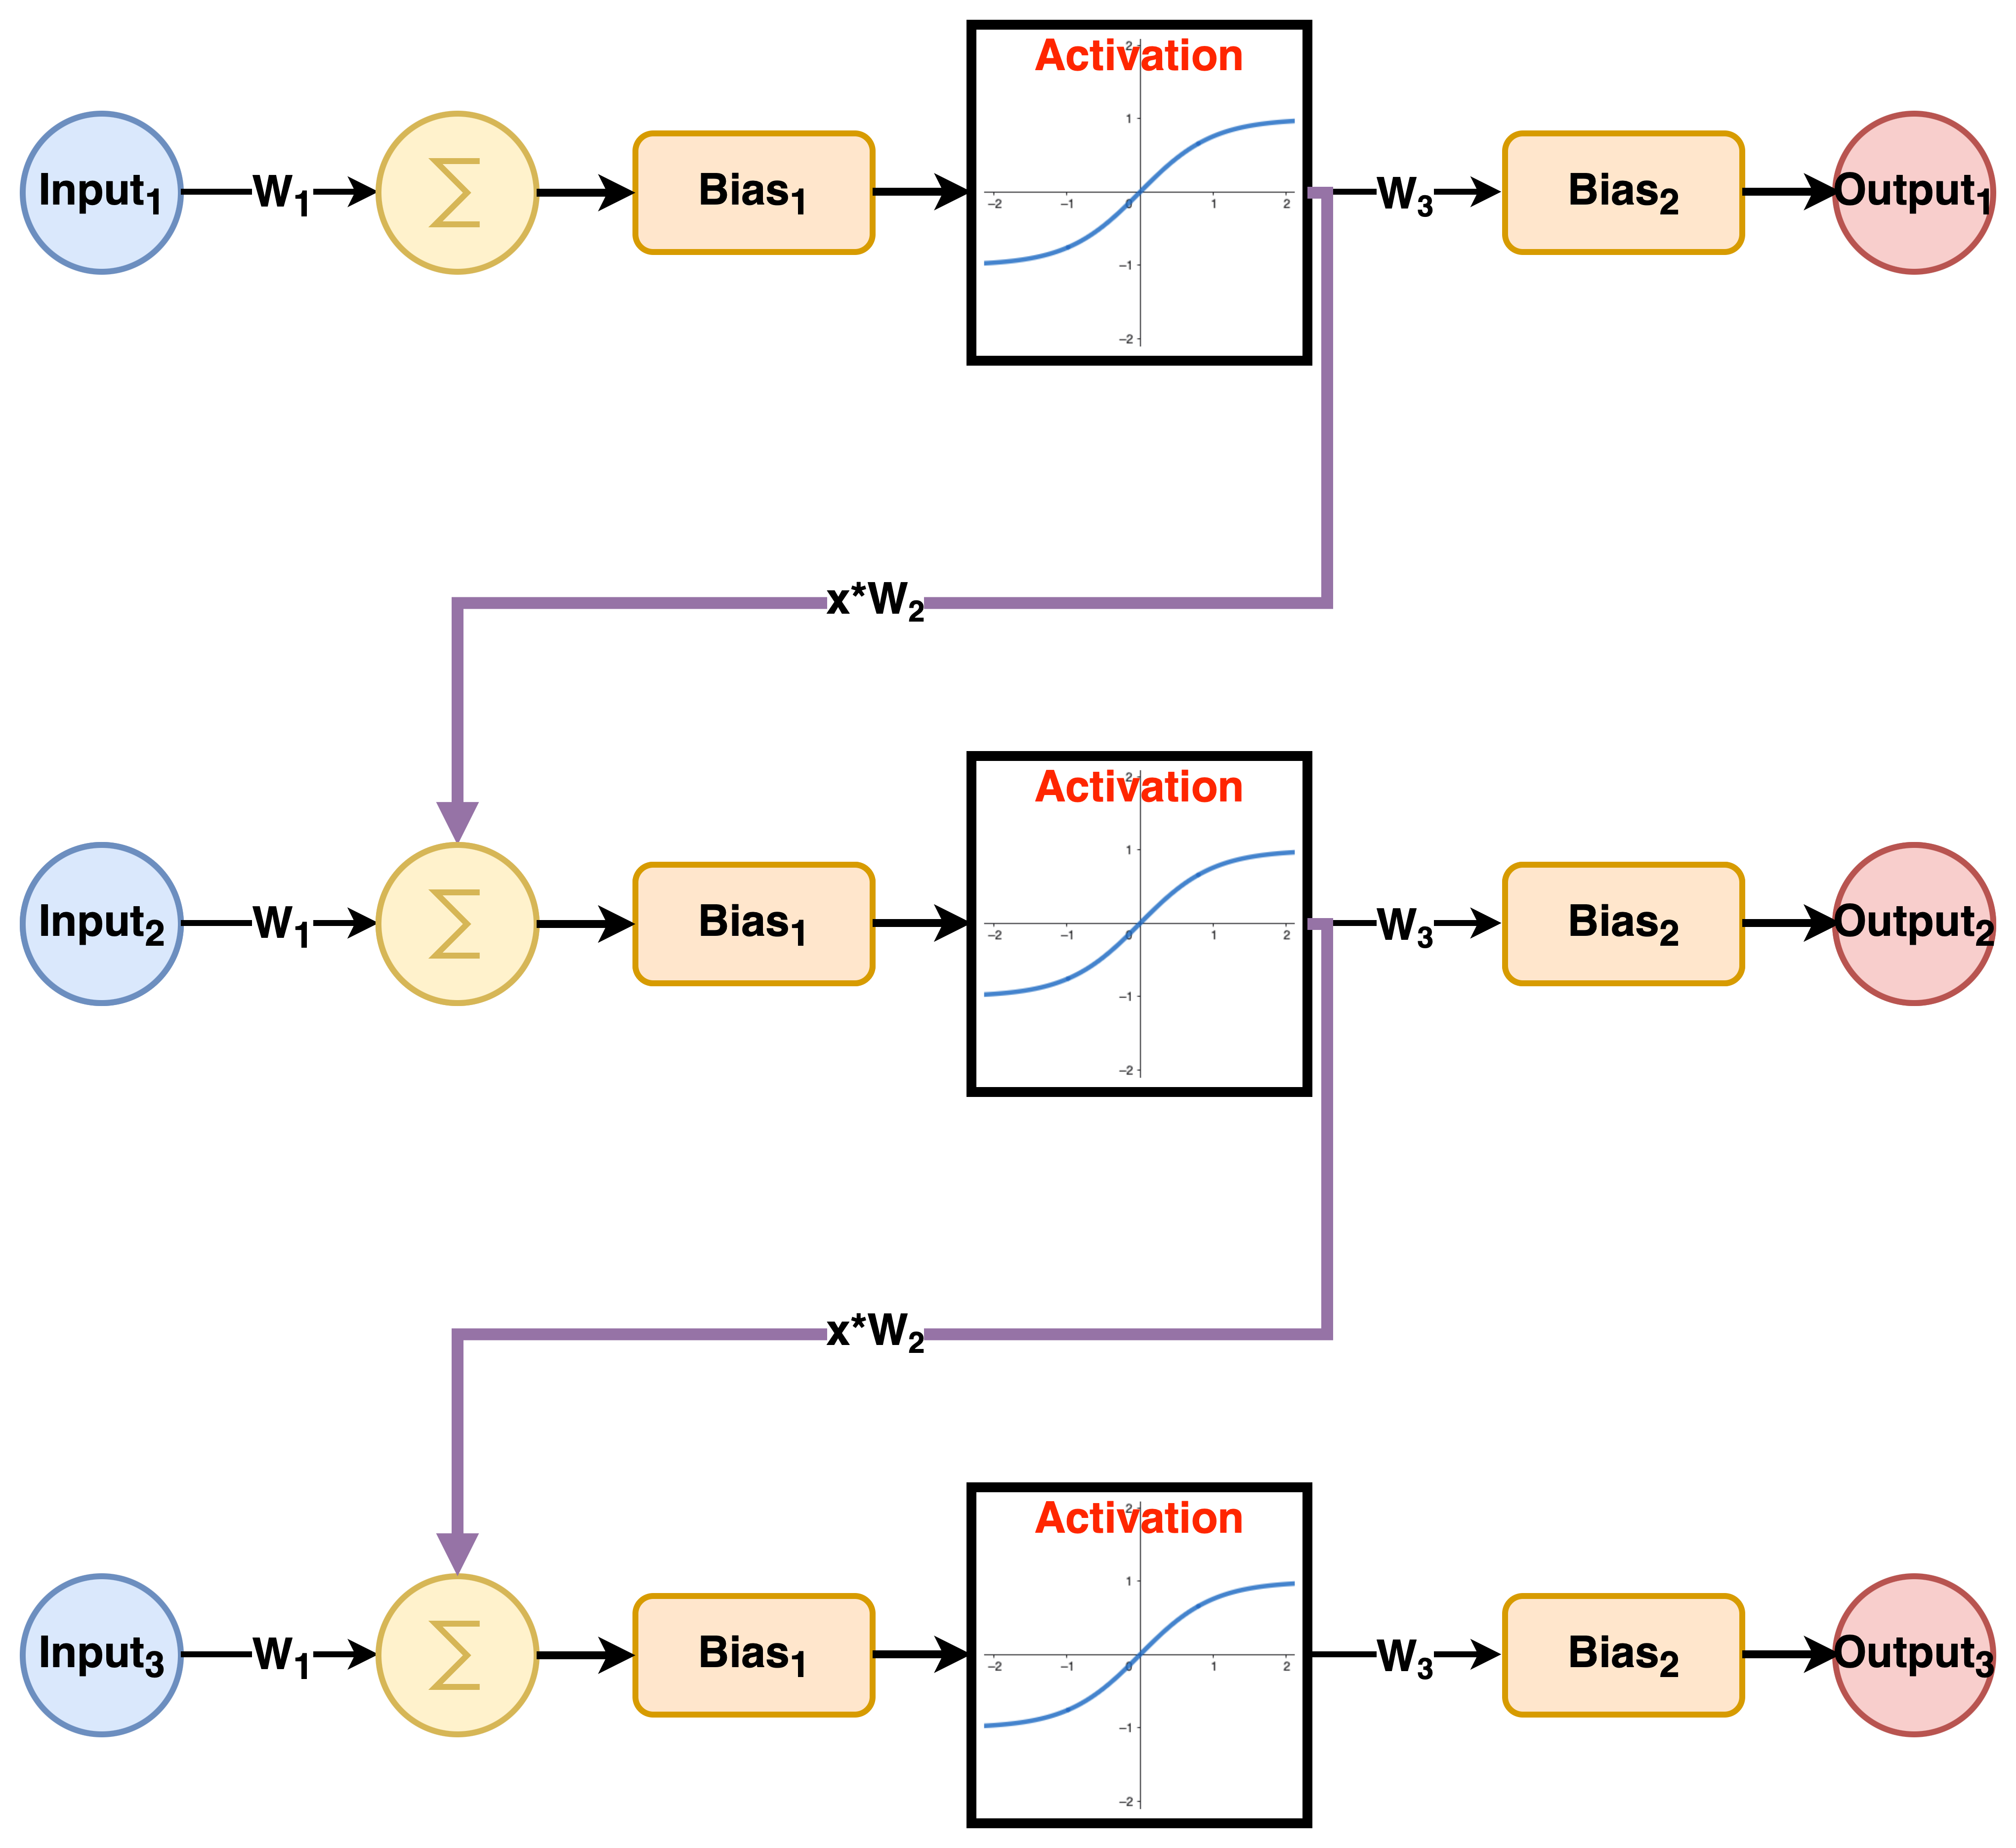
\includegraphics[width=0.8\linewidth]{img/rnn_unrolled.png}
\caption{Unrolled RNN with three states.}
\label{fig:rnn_unrolled}
\end{figure}

As can be observed, each feedback loop is added to the subsequent input (multiplied by $W_1$) \cite{medium_math_rnn}. This structure implies that the output of each single state $output_t$ is influenced not only by the current input $input_t$, but also by all previous inputs, since the state at step $t-1$ incorporates information accumulated from all preceding steps \cite{quarkml-rnn-explained}.
In a context where a decision or prediction based on the entire sequence is desired, $output_T$ is typically chosen precisely because it constitutes a complete representation that takes all previous states into account \cite{cs231n-rnn}.

\subsection{Mathematical Foundations of RNNs}
\noindent
Mathematically, an RNN can be represented through the recurrence formula \cite{cs231n-rnn, medium_math_rnn}:
\begin{equation}
h_t = f_W (h_{t-1}, x_t)
\end{equation}

where:
\begin{itemize}
    \item $h_t$ represents the hidden state at time step $t$
    \item $h_{t-1}$ represents the hidden state at time step $t-1$
    \item $x_t$ represents the input at time step $t$
    \item $f_W$ represents the state transition function with parameters $W$
\end{itemize}

The most elementary form of RNN, called \textbf{Vanilla RNN}, uses a single hidden state update formula \cite{cs231n-rnn}:
\begin{equation}
h_t = \tanh(W_{hh} h_{t-1} + W_{xh} x_t + b_h)
\label{formula:hidden_state_rnn}
\end{equation}


In matrix form:
\begin{equation}
\underbrace{
\begin{pmatrix} \bullet \\ \bullet \\ \bullet \\ \bullet \end{pmatrix}
}_{\mathbf{h}_t}
= \tanh \left(
\underbrace{
\begin{pmatrix}
\bullet & \bullet & \bullet & \bullet \\
\bullet & \bullet & \bullet & \bullet \\
\bullet & \bullet & \bullet & \bullet \\
\bullet & \bullet & \bullet & \bullet
\end{pmatrix}
}_{\mathbf{W}_{hh}}
\cdot
\underbrace{
\begin{pmatrix} \bullet \\ \bullet \\ \bullet \\ \bullet \end{pmatrix}
}_{\mathbf{h}_{t-1}}
+
\underbrace{
\begin{pmatrix}
\bullet & \bullet & \bullet \\
\bullet & \bullet & \bullet \\
\bullet & \bullet & \bullet \\
\bullet & \bullet & \bullet
\end{pmatrix}
}_{\mathbf{W}_{xh}}
\cdot
\underbrace{
\begin{pmatrix} \bullet \\ \bullet \\ \bullet \end{pmatrix}
}_{\mathbf{x}_t}
+
\underbrace{
\begin{pmatrix} \bullet \\ \bullet \\ \bullet \\ \bullet \end{pmatrix}
}_{\mathbf{b}_h}
\right)
\end{equation}

where:
\begin{itemize}
\item $W_{hh}$ represents the weight matrix for recurrent connections
\item $W_{xh}$ represents the weight matrix for input sequences
\item $b_h$ represents the hidden layer bias
\end{itemize}

Essentially, the sum of the projections of the weight matrices $W_{hh}$ and $W_{xh}$, for $h_{t-1}$ and $x_t$ respectively, is compressed through the $\tanh$ (hyperbolic tangent) function, which serves as the \textbf{\textit{activation function}} \cite{medium_math_rnn}. The result of this operation constitutes the hidden state $h_t$ of the RNN \cite{cs231n-rnn}.

Considering the most elementary case, it is possible to base predictions directly on $h_t$ by simply performing a final transformation \cite{medium_math_rnn, quarkml-rnn-explained}:
\begin{equation}
o_t = W_{ho}h_t + b_o
\end{equation}


In matrix form:
\begin{equation}
\underbrace{
\begin{pmatrix} \bullet \\ \bullet \end{pmatrix}
}_{\mathbf{o}_t}
=
\underbrace{
\begin{pmatrix}
\bullet & \bullet & \bullet & \bullet \\
\bullet & \bullet & \bullet & \bullet
\end{pmatrix}
}_{\mathbf{W}_{ho}}
\cdot
\underbrace{
\begin{pmatrix} \bullet \\ \bullet \\ \bullet \\ \bullet \end{pmatrix}
}_{\mathbf{h}_t}
+
\underbrace{
\begin{pmatrix} \bullet \\ \bullet \end{pmatrix}
}_{\mathbf{b}_o}
\end{equation}

where:
\begin{itemize}
\item $W_{ho}$ represents a weight matrix (hidden-to-output)
\item $b_o$ represents the output bias
\item $o_t$ represents the vector of output logits from the model at time $t$
\end{itemize}

The weight matrices $W_{hh}$, $W_{xh}$, and $W_{ho}$ are learned via \textbf{Backpropagation Through Time} (BPTT) \cite{quarkml-bptt}, an extension of the traditional backpropagation algorithm adapted for training Recurrent Neural Networks.

\subsubsection{Practical Case Study: Character-Level Modeling}
To provide a more practical understanding of how an RNN operates, we illustrate its functioning step-by-step as a Character-Level Language Model \cite{cs231n-rnn}. In this example (for simplicity), the bias vectors are set with all elements to zero: $b_h = [0,0,...,0]^T,b_o = [0,0,...,0]^T$. The objective is to show how an RNN, given a sequence of characters, predicts the next character. At each time step, the network must provide a probability distribution over the vocabulary characters, indicating which character should come next in the sequence \cite{cs231n-rnn, quarkml-rnn-explained}.

The computation process develops in the following phases:
\begin{enumerate}
\item \textbf{Vocabulary Construction:} A vocabulary containing all unique characters present in the training corpus is defined \cite{cs231n-rnn}.

\item \textbf{Input Representation:} Each character in the vocabulary is transformed into a numerical representation. A common technique is one-hot encoding, where each character corresponds to a binary vector with a single element equal to 1 and all others to 0. The vector dimension is equal to the vocabulary size \cite{quarkml-rnn-explained}.

\item \textbf{Computation Process:} At each time step $t$, the RNN receives the one-hot vector of the current character $x_t$ and the hidden state of the previous step $h_{t-1}$ as input. Its task is to produce an output $y_t$ representing a probability distribution over the next character $x_{t+1}$ \cite{cs231n-rnn, medium_math_rnn}.

\end{enumerate}

We use the input sequence \texttt{hello} as an example; the RNN's task will therefore be to:
\begin{itemize}
\item Given \texttt{"h"} predict \texttt{"e"}
\item Given \texttt{"he"} predict \texttt{"l"}
\item Given \texttt{"hel"} predict \texttt{"l"}
\item Given \texttt{"hell"} predict \texttt{"o"}
\end{itemize}
Note that, in this case, the training corpus consists solely of the string \texttt{hello} with a vocabulary $V=\{\texttt{``h''}, \texttt{``e''}, \texttt{``l''}, \texttt{``o''}\}$ of four characters.

Each character in the vocabulary is represented using \textbf{one-hot} encoding, i.e., through vectors in which only one element is \textit{\textbf{1}} and all others are \textit{\textbf{0}}. The length of each vector is equal to the vocabulary cardinality, in this case $|V|=4$:
\[
\begin{bmatrix} 1 \\ 0 \\ 0 \\ 0 \end{bmatrix} = \text{``h''} \quad
\begin{bmatrix} 0 \\ 1 \\ 0 \\ 0 \end{bmatrix} = \text{``e''} \quad
\begin{bmatrix} 0 \\ 0 \\ 1 \\ 0 \end{bmatrix} = \text{``l''} \quad
\begin{bmatrix} 0 \\ 0 \\ 0 \\ 1 \end{bmatrix} = \text{``o''}
\]

The core of the process is the recursive update of the hidden state through \\ $h_t = \tanh(W_{hh} h_{t-1} + W_{xh} x_t)$ which, setting the weight matrices $W$ to \textit{random} values, develops as:

\begin{align}
\begin{bmatrix} 0.3 \\ -0.1 \\ 0.9 \end{bmatrix} &= f_W \left( W_{hh} \begin{bmatrix} 0 \\ 0 \\ 0 \end{bmatrix} + W_{xh} \begin{bmatrix} 1 \\ 0 \\ 0 \\ 0 \end{bmatrix} \right) \tag{$h_1$} \\[1.5em]
\begin{bmatrix} 1.0 \\ 0.3 \\ 0.1 \end{bmatrix} &= f_W \left( W_{hh} \begin{bmatrix} 0.3 \\ -0.1 \\ 0.9 \end{bmatrix} + W_{xh} \begin{bmatrix} 0 \\ 1 \\ 0 \\ 0 \end{bmatrix} \right) \tag{$h_2$} \\[1.5em]
\begin{bmatrix} 0.1 \\ -0.5 \\ -0.3 \end{bmatrix} &= f_W \left( W_{hh} \begin{bmatrix} 1.0 \\ 0.3 \\ 0.1 \end{bmatrix} + W_{xh} \begin{bmatrix} 0 \\ 0 \\ 1 \\ 0 \end{bmatrix} \right) \tag{$h_3$} \\[1.5em]
\begin{bmatrix} -0.3 \\ 0.9 \\ 0.7 \end{bmatrix} &= f_W \left( W_{hh} \begin{bmatrix} 0.1 \\ -0.5 \\ -0.3 \end{bmatrix} + W_{xh} \begin{bmatrix} 0 \\ 0 \\ 1 \\ 0 \end{bmatrix} \right) \tag{$h_4$}
\end{align}

The output is then calculated iteratively, in the form of scores (\textit{logits}) at time $t$, for each single $h_t$ using $y_t = W_{ho}h_t$:

\begin{figure}[H]
\centering
\begin{tikzpicture}[
node distance=1.5cm and 1cm,
input/.style={rectangle, draw, fill=red!15, minimum height=1.6cm, minimum width=1cm, align=center, font=\small},
hidden/.style={rectangle, draw, fill=green!15, minimum height=1.2cm, minimum width=1cm, align=center, font=\small},
output/.style={rectangle, draw, fill=blue!15, minimum height=1.6cm, minimum width=1cm, align=center, font=\small},
io_char/.style={align=center, font=\small},
layer_label/.style={text width=2.5cm, align=right, font=\small\bfseries},
weight_label/.style={midway, fill=white, inner sep=1pt, font=\tiny},
]

% Layer Labels
\node[layer_label, text=red!60!black] at (-2, -2.5) {input layer};
\node[layer_label, text=green!50!black] at (-2, 0) {hidden layer};
\node[layer_label, text=blue!60!black] at (-2, 2.5) {output layer};

% Time Step 1 (h) -> e
\node[input] (x1) at (0, -2.5) {$1$\\$0$\\$0$\\$0$};
\node[io_char] (char_x1) [below=0.1cm of x1] {``h''};
\node[hidden] (h1) at (0, 0) {$0.3$\\$-0.1$\\$0.9$};
\node[output] (y1) at (0, 2.5) {\color{red} $1.0$\\ \color{green!50!black} $2.2$\\ \color{red} $-3.0$\\ \color{red}$4.1$};
\node[io_char] (char_y1) [above=0.1cm of y1] {``e''};

% Time Step 2 (e) -> l
\node[input] (x2) [right=2cm of x1] {$0$\\$1$\\$0$\\$0$};
\node[io_char] (char_x2) [below=0.1cm of x2] {``e''};
\node[hidden] (h2) [right=2cm of h1] {$1.0$\\$0.3$\\$0.1$};
\node[output] (y2) [right=2cm of y1] {\color{red} $0.5$\\ \color{red} $0.3$\\ \color{green!50!black} $-1.0$\\ \color{red} $1.2$};
\node[io_char] (char_y2) [above=0.1cm of y2] {``l''};

% Time Step 3 (l) -> l
\node[input] (x3) [right=2.05cm of x2] {$0$\\$0$\\$1$\\$0$};
\node[io_char] (char_x3) [below=0.1cm of x3] {``l''};
\node[hidden] (h3) [right=2cm of h2] {$0.1$\\$-0.5$\\$-0.3$};
\node[output] (y3) [right=2cm of y2] {\color{red} $0.1$\\\color{red} $0.5$\\ \color{green!50!black} $1.9$\\ \color{red} $-1.1$};
\node[io_char] (char_y3) [above=0.1cm of y3] {``l''};

% Time Step 4 (l) -> o
\node[input] (x4) [right=2.05cm of x3] {$0$\\$0$\\$1$\\$0$};
\node[io_char] (char_x4) [below=0.1cm of x4] {``l''}; % Note: image has 'l' as input for 'o'
\node[hidden] (h4) [right=2cm of h3] {$-0.3$\\$0.9$\\$0.7$};
\node[output] (y4) [right=2cm of y3] {\color{red} $0.2$\\ \color{red} $-1.5$\\ \color{red} $-0.1$\\ \color{green!50!black} $2.2$};
\node[io_char] (char_y4) [above=0.1cm of y4] {``o''};

% Arrows and Weight Labels
% Input to Hidden
\draw[-{Stealth[length=2mm]}, red!60!black] (x1) -- (h1) node[weight_label, pos=0.8, right=1mm] {$W_{xh}$};
\draw[-{Stealth[length=2mm]}, red!60!black] (x2) -- (h2);
\draw[-{Stealth[length=2mm]}, red!60!black] (x3) -- (h3);
\draw[-{Stealth[length=2mm]}, red!60!black] (x4) -- (h4);

% Hidden to Hidden
\draw[-{Stealth[length=2mm]}, green!50!black] (h1) -- (h2) node[weight_label, pos=0.6, above=1mm] {$W_{hh}$};
\draw[-{Stealth[length=2mm]}, green!50!black] (h2) -- (h3);
\draw[-{Stealth[length=2mm]}, green!50!black] (h3) -- (h4);

% Hidden to Output
\draw[-{Stealth[length=2mm]}, blue!60!black] (h1) -- (y1) node[weight_label, pos=0.8, right=1mm] {$W_{hy}$};
\draw[-{Stealth[length=2mm]}, blue!60!black] (h2) -- (y2);
\draw[-{Stealth[length=2mm]}, blue!60!black] (h3) -- (y3);
\draw[-{Stealth[length=2mm]}, blue!60!black] (h4) -- (y4);

\end{tikzpicture}
\caption{Calculation of \textit{logits} by processing the sequence \texttt{``hell''} for each $h_t$.}
\end{figure}

The acquired scores are then normalized using a function, typically \textbf{softmax} $\sigma(o_t)$, to obtain a probability distribution. 
\[
\begin{array}{c}
\text{\textit{Output layer}} \\
\begin{bmatrix} 1.0 \\ 2.3 \\ -3.0 \\ 4.1 \end{bmatrix}
\end{array}
\quad \rightarrow \quad
\begin{array}{c}
\text{\textbf{softmax}} \\
\sigma(o_t) = \displaystyle\frac{e^{o_{i}}}{\sum_{j=1}^{|V|} e^{o_{j}}} \quad i = 1,\dots,|V|
\end{array}
\quad \rightarrow \quad
\begin{array}{c}
\text{\textit{Probabilities}} \\
\begin{bmatrix} 0.03719 \\ 0.13648 \\ 0.00068 \\ 0.82565 \end{bmatrix}
\end{array}
\]

During training, the error between the predicted distribution and the target character (represented as a one-hot vector) is calculated via a cost function such as \textbf{cross-entropy} \cite{cs231n-rnn, quarkml-bptt}. This error is then minimized by updating the network weights through \textbf{Backpropagation Through Time} \cite{quarkml-bptt, cs231n-rnn}.

This mechanism allows the network not only to associate an input with an output but to do so in a context-dependent manner \cite{cs231n-rnn}. \footnote{Naturally, with random weights, the prediction is likely wrong. The next section explains how BPTT iteratively adjusts these matrices to minimize the error shown in the example \cite{quarkml-bptt}.}% Ad esempio, nel predire il carattere dopo la prima \texttt{"l"} di \texttt{"hello"}, la rete deve produrre un'altra \texttt{"l"}, mentre dopo la seconda deve produrre una \texttt{"o"}. Questa distinzione è possibile solo grazie all'informazione contestuale accumulata nell'hidden state.
\bigskip

\subsection{Backpropagation Through Time}
The goal of BPTT is to minimize the total loss of an output sequence (with respect to the correct output sequence) by backpropagating the error from the outputs to the respective hidden states and, through recurrence, from future states to past ones \cite{quarkml-bptt}. The shared nature of the weights implies that each parameter receives the sum of contributions from all time steps in which it is used \cite{quarkml-bptt}.

To apply backpropagation, it is necessary to transform the cyclic nature of the RNN into a \textbf{FeedForward} (thus acyclic) structure; the resulting RNN is called an Unrolled RNN \cite{quarkml-bptt, cs231n-rnn}.

To obtain an Unrolled RNN starting from a classic RNN \cite{quarkml-rnn-explained}:
\begin{itemize}
\item The RNN is "unrolled" along the time sequence.
\item Each time step $t$ becomes a layer of the network.
\item Weights are shared across all temporal layers.
\end{itemize}

An unrolled RNN can be visualized in Figure \ref{fig:rnn}; the state \textit{"state 0"} represents the initial state of the RNN. The initial state is typically set as a vector of all zeros \cite{cs231n-rnn}.

\begin{figure}[H]
\centering
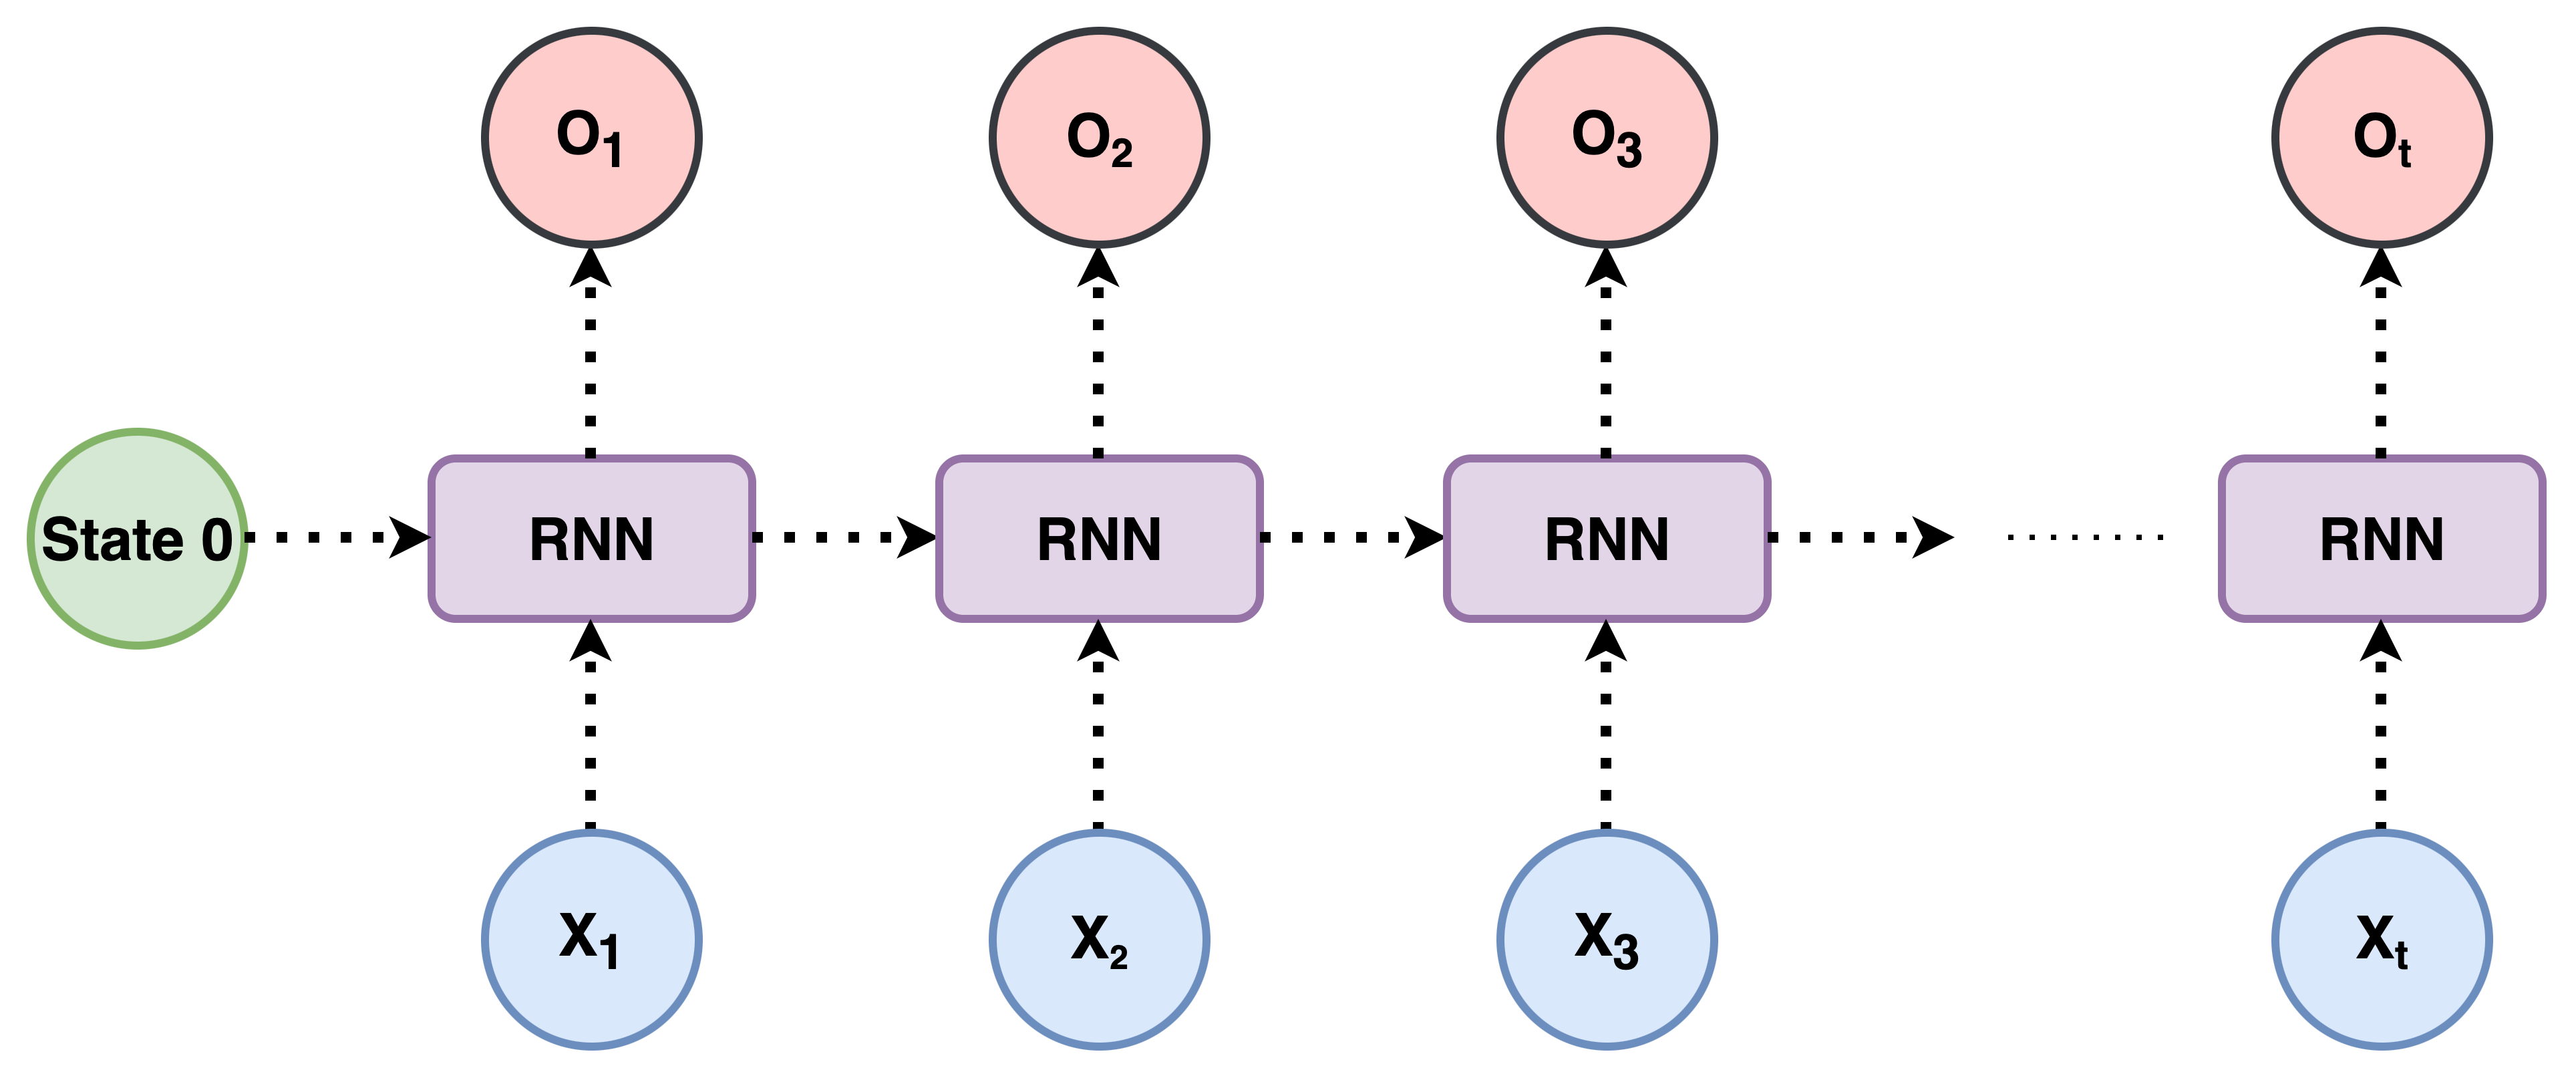
\includegraphics[width=0.8\linewidth]{img/rnn_o.png}
\caption{Graphical representation of an Unrolled Vanilla RNN.}
\label{fig:rnn}
\end{figure}

Considering a vanilla RNN with activation function $\phi$, we define:
$$
h_t = \phi(W_{xh} X_t + W_{hh} h_{t-1} + b_h), \quad o_t=W_{ho}h_t+b_o, \quad \hat{y}=\text{softmax}(o_t)
$$
where:
\begin{itemize}
\item $\phi$ represents the activation function
\item $\hat{y}_t$ represents the predicted probability vector at time $t$
\end{itemize}

The steps of the BPTT algorithm are as follows \cite{quarkml-bptt}:

\paragraph{Forward Pass} For each time step $t$ from $1$ to $T$, the following quantities are calculated \cite{medium_math_rnn, quarkml-bptt}:

\begin{itemize}
\item Hidden state $\rightarrow h_t = \phi(W_{xh} X_t + W_{hh} h_{t-1} + b_h)$
\item Output logits $\rightarrow o_t=W_{ho}h_t+b_o$ % Nota: Ho corretto h_o in h_t come discusso prima, se preferisci l'originale rimetti h_o
\item Predicted probabilities $\hat{y}=\text{softmax}(o_t)$
\end{itemize}
The aggregate loss $L$, i.e., the sum of the loss functions calculated at each individual time step of the sequence, is given by \cite{quarkml-bptt}:
\begin{equation}
L =\sum^T_{t=1} \ell_t(o_t, y_t)
\end{equation}
where:
\begin{itemize}
\item $\ell_t$ represents the loss function calculated at time step $t$
\item $y_t$ represents the correct result (ground truth)
\end{itemize}

In this case, we set $L=\text{MSE}$, \footnote{Although Cross-Entropy is the standard loss function for multi-class classification tasks, Mean Squared Error (MSE) is adopted here to simplify the mathematical derivation of the gradients \cite{quarkml-bptt}.} yielding:
\begin{equation}
L = \frac{1}{T} \sum^T_{t=1}(y-o_t)^2
\end{equation}

\paragraph{Backward Pass (Gradient Calculation)}
Gradients are calculated by proceeding backward in time.
Thus, we start from the final step $T$ until reaching the initial step $1$ \cite{quarkml-bptt, cs231n-rnn}.

Calculating the derivative of $L$ with respect to the output $o_t$, we obtain:
\begin{equation}
\frac{\partial L}{\partial o_t} = \frac{2}{n}\sum^n_{k=t}(y-o_k) % Ho corretto l'indice della somma per chiarezza matematica (k invece di t=t)
\end{equation}
where:
\begin{itemize}
\item $n = T-t+1$ is the number of elements in the subsequence ranging from $t$ to $T$
\end{itemize} \cite{quarkml-bptt}
The derivative just found represents how much and in which direction a change in the output $o_t$ influences the overall network error. In other words, it is the gradient indicating whether $o_t$ needs to be increased or decreased to reduce the model's loss \cite{medium_math_rnn}.

At this point, it is necessary to recall that the goal of BPTT is to find the optimal weights (and biases) at each update in the considered RNN. To achieve this goal, it is necessary to use gradient descent \cite{quarkml-bptt}.

The terms of the RNN that condition the change of weights $W$ are \cite{medium_math_rnn, quarkml-bptt}:
\begin{itemize}
 \item The change of $L$ with respect to the change in output $o_t$, measured by: $$\frac{\partial L}{\partial o_t}$$
 \item The change of output $o_t$ with respect to the change in hidden states $h_t$, measured by: $$\frac{\partial o_t}{\partial h_t}$$
\item The change of hidden states with respect to the change in weights $W$, measured by: $$\frac{\partial h_t}{\partial W}$$
\end{itemize}

The considerations just concluded constitute one of the most important rules of differential calculus in machine learning: the \textbf{Chain Rule} \cite{medium_math_rnn, quarkml-bptt}.
Ideally, the chain rule allows us to calculate how the variation of an internal parameter (for example, a weight of a neural network) affects the final output and, consequently, the loss function \cite{quarkml-bptt}.
\begin{figure}[H]
\centering
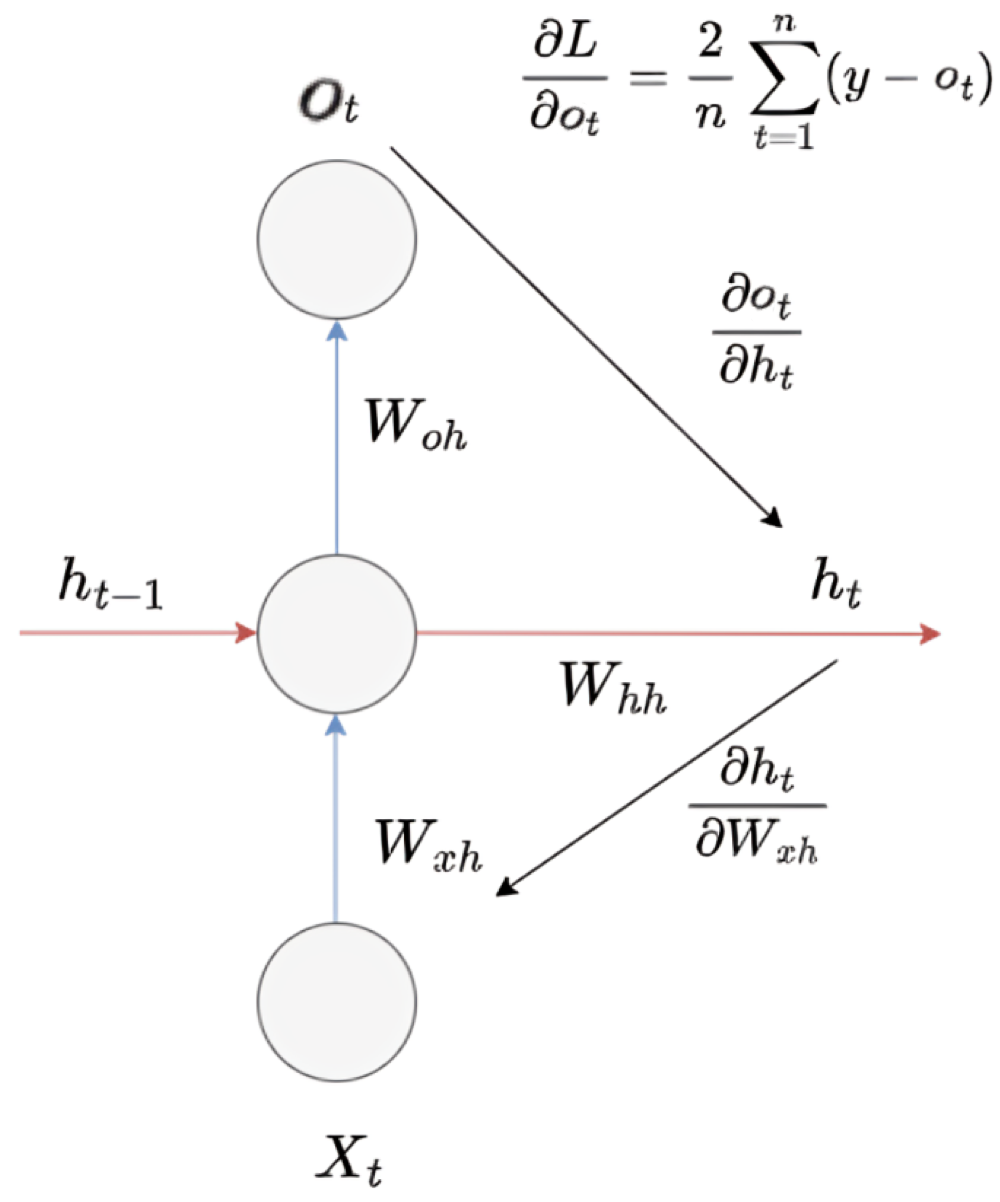
\includegraphics[width=0.4\linewidth]{img/bptt_single3.png}
\caption{Gradient flow in a single time step $t$}
\label{fig:bptt_single}
\end{figure}

Considering the weight matrix $W_{xh}$, in formula, we obtain \cite{medium_math_rnn, quarkml-bptt}:
\begin{equation}
\frac{\partial L}{\partial W_{xh}} = \frac{\partial L}{\partial o_{t}}\frac{\partial o_t}{\partial h_{t}}\frac{\partial h_t}{\partial W_{xh}}
\end{equation}

This formula therefore allows us to calculate the gradient of the loss in relation to the input weights $W_{xh}$ within a \textbf{single time step $t$} \cite{quarkml-bptt}.

When dealing with multiple time steps, it is necessary to sum each individual gradient \cite{quarkml-bptt}.
\begin{figure}[H]
\centering
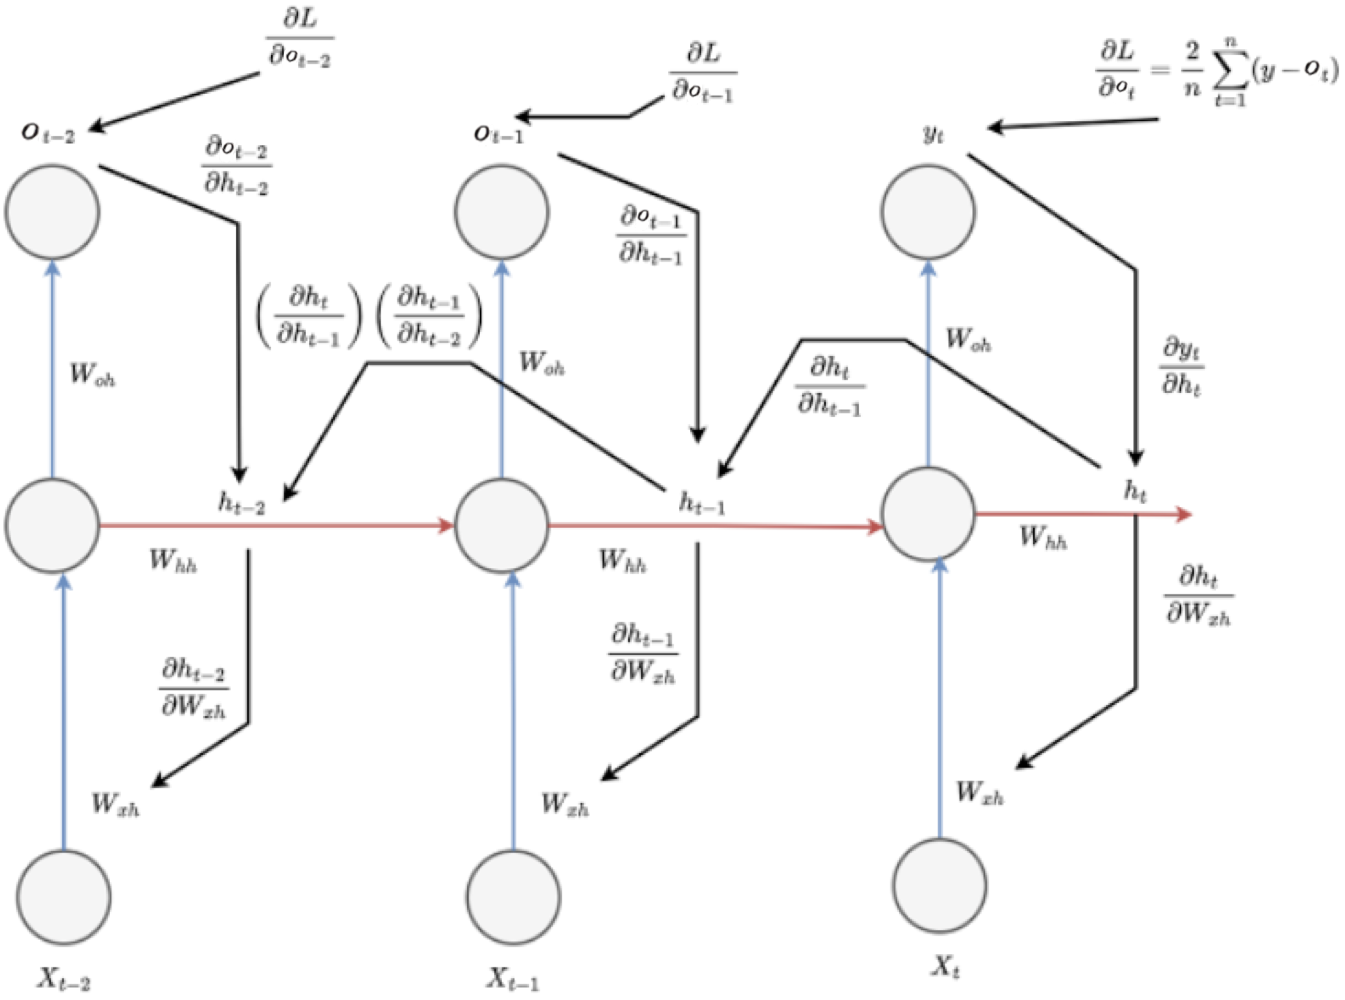
\includegraphics[width=0.8\linewidth]{img/bptt_multiple_2.png}
\caption{Gradient flow over three time steps $t-2, t-1, t$}
\label{fig:bptt_multiple_2}
\end{figure}
Applying the chain rule, we therefore obtain \cite{medium_math_rnn, quarkml-bptt}:
\begin{itemize}
\item \textbf{One time step:}
$$\frac{\partial L}{\partial W_{xh}} = \underbrace{ \frac{\partial L}{\partial o_{t}}\frac{\partial o_t}{\partial h_{t}}\frac{\partial h_t}{\partial W_{xh}}}_{i=0}$$
\item \textbf{Two time steps:} 
$$
\frac{\partial L}{\partial W_{xh}} = 
\underbrace{
\frac{\partial L}{\partial o_t} 
\frac{\partial o_t}{\partial h_t} 
\frac{\partial h_t}{\partial W_{xh}}
}_{i=0} + 
\underbrace{
\frac{\partial L}{\partial o_{t-1}} 
\frac{\partial o_{t-1}}{\partial h_{t-1}} 
\left( \frac{\partial h_t}{\partial h_{t-1}} \right) 
\frac{\partial h_{t-1}}{\partial W_{xh}}
}_{i=1}
$$

\item \textbf{Three time steps:}
$$
\frac{\partial L}{\partial W_{xh}} = 
\underbrace{
\frac{\partial L}{\partial o_t} 
\frac{\partial o_t}{\partial h_t} 
\frac{\partial h_t}{\partial W_{xh}}
}_{i=0} + 
\underbrace{
\frac{\partial L}{\partial o_{t-1}} 
\frac{\partial o_{t-1}}{\partial h_{t-1}} 
\left( \frac{\partial h_t}{\partial h_{t-1}} \right) 
\frac{\partial h_{t-1}}{\partial W_{xh}}
}_{i=1} +
$$
$$
+\underbrace{
\frac{\partial L}{\partial o_{t-2}} 
\frac{\partial o_{t-2}}{\partial h_{t-2}} 
\left( \frac{\partial h_t}{\partial h_{t-1}} \right) 
\left( \frac{\partial h_{t-1}}{\partial h_{t-2}} \right)
\frac{\partial h_{t-2}}{\partial W_{xh}}
}_{i=2}
$$
\end{itemize}

%%%%%%%%%%%%%%%%%%%%%%%%%%%
%Completa questa sezione per bene e poi riparti dai bias
%%%%%%%%%%%%%%%%%%%%%%%%%%%
As the number of time steps increases, the number of gradients increases accordingly. The general formula for calculating $\frac{\partial L}{\partial W_{xh}}$ at time step $t$ is \cite{quarkml-bptt}:
\begin{equation}
\frac{\partial L}{\partial W_{xh}} = \sum_{i=0}^{t} \left[ \underbrace{\frac{\partial L}{\partial o_{t-i}} \frac{\partial o_{t-i}}{\partial h_{t-i}}}_{R_{t-i}} \left( \prod_{j=(t-i+1)}^{t} \frac{\partial h_j}{\partial h_{j-1}} \right) \underbrace{\frac{\partial h_{t-i}}{\partial W_{xh}}}_{S_{t-i}} \right]
\label{eq:grad_wxh}
\end{equation}

where:
\begin{itemize}
\item $o_{t-i}$ represents the output at time step $t-i$
\item $h_{t-i}$ represents the hidden state at time step $t-i$
\item $R_{t-i}$ represents how the variation of the hidden state at time $t-i$ influences the loss through the output at that same instant
\item $S_{t-i}$ represents the direct effect of the weight $W_{xh}$ on the hidden state at time $t-i$
\end{itemize}

To find the derivative of the loss with respect to the weights $W_{hh}$, it is sufficient to replace $W_{xh}$ with $W_{hh}$ in the previous equation, yielding:
\begin{equation}
\frac{\partial L}{\partial W_{hh}} = \sum_{i=0}^{t} \left[ \underbrace{\frac{\partial L}{\partial o_{t-i}} \frac{\partial o_{t-i}}{\partial h_{t-i}}}_{R_{t-i}} \left( \prod_{j=(t-i+1)}^{t} \frac{\partial h_j}{\partial h_{j-1}} \right) \underbrace{\frac{\partial h_{t-i}}{\partial W_{hh}}}_{T_{t-i}} \right]
\end{equation}

where:
\begin{itemize}
\item $T_{t-i}$ represents the extent to which the recurrent weight $W_{hh}$ influences the hidden state at step $t-i$
\end{itemize}

To find the derivative of the output layer weights $W_{oh}$, it is sufficient to consider $o_t$ and $W_{oh}$, resulting in:
\begin{equation}
\frac{\partial L}{\partial W_{oh}} = \sum_{i=0}^{t} \frac{\partial L}{\partial o_{t-i}} \frac{\partial o_{t-i}}{\partial W_{oh}}
\label{eq:grad_woh}
\end{equation}

We now need to find the derivatives of the hidden layer bias $b_h$ and the output layer bias $b_o$.

Regarding the calculation of $b_h$, it is sufficient to replace the matrix $W_{xh}$ with $b_h$ in Equation \ref{eq:grad_wxh}:
\begin{equation}
 \frac{\partial L}{\partial b_{h}} = \sum_{i=0}^{t} \left[ \underbrace{\frac{\partial L}{\partial o_{t-i}} \frac{\partial o_{t-i}}{\partial h_{t-i}}}_{R_{t-i}} \left( \prod_{j=(t-i+1)}^{t} \frac{\partial h_j}{\partial h_{j-1}} \right) \underbrace{\frac{\partial h_{t-i}}{\partial b_{h}}}_{\phi'(a_{t-i})} \right]
\end{equation}

where:
\begin{itemize}
\item $\phi'(a_{t-i})$ represents the derivative of the activation function $\phi$ evaluated at point $a_{t-i}$
\item $a_{t-i}$ is the linear input to the recurrent neuron at time $t-i$, in this case $a_{t-i}=W_{xh}x_{t-i} + W_{hh} h_{t-i-1} + b_h $
\end{itemize}

Similarly, $b_o$ can be found by substituting into Equation \ref{eq:grad_woh}:
\begin{equation}
\frac{\partial L}{\partial b_{o}} = \sum_{i=0}^{t} \frac{\partial L}{\partial o_{t-i}} \frac{\partial o_{t-i}}{\partial b_{o}}
\end{equation}

\paragraph{Weight and Bias Update} The update of weights and biases is performed via gradient descent or one of its optimizers (e.g., Adam) \cite{quarkml-bptt}:
\begin{equation}
 \theta_{k+1} = \theta_k - \eta \nabla L(\theta_k)
\end{equation}

where:
\begin{itemize}
\item $\theta_{k+1}$ represents the vector of updated parameters at iteration $k+1$
\item $\theta_{k}$ represents the vector of parameters at the current iteration $k$
\item $\eta$ represents the learning rate, a positive scalar determining the step size to take in the direction opposite to the gradient
\item $\nabla L(\theta_{k})$ represents the gradient of the cost function $L$ calculated with respect to parameters $\theta_k$. It indicates the direction of steepest ascent of the function.
\end{itemize}

Applying this to the weights $W$ and biases $b$ of the RNN under consideration:

\begin{itemize}
\item \textbf{Updating $\boldsymbol{W_{oh}}$}: 
$$
W_{oh} \leftarrow W_{oh} -\eta \cdot \frac{\partial L}{\partial W_{oh}}
$$

\item \textbf{Updating $\boldsymbol{W_{xh}}$}: 
$$
W_{xh} \leftarrow W_{xh} -\eta \cdot \frac{\partial L}{\partial W_{xh}}
$$

\item \textbf{Updating $\boldsymbol{W_{hh}}$}: 
$$
W_{hh} \leftarrow W_{hh} -\eta \cdot \frac{\partial L}{\partial W_{hh}}
$$

\item \textbf{Updating $\boldsymbol{b_{h}}$}: 
$$
b_{h} \leftarrow b_{h} -\eta \cdot \frac{\partial L}{\partial b_{h}}
$$

\item \textbf{Updating $\boldsymbol{b_{o}}$}: 
$$
b_{o} \leftarrow b_{o} -\eta \cdot \frac{\partial L}{\partial b_{o}}
$$


\end{itemize}

To conclude, the complete pseudocode for BPTT is provided below:

\begin{algorithm}[H]
\caption{Backpropagation Through Time (BPTT)}
\label{alg:bptt}
\small

\begin{algorithmic}[1]

\Inputs
\Statex $\mathbf{a} = (a_0, a_1, \dots, a_{T-1})$ \Comment{Input sequence}
\Statex $\mathbf{y} = (y_0, y_1, \dots, y_{T-1})$ \Comment{Target sequence}
\Statex $N_{epochs}$ \Comment{Maximum number of training epochs}
\Statex $\eta$ \Comment{Learning rate}
\Statex $T$ \Comment{Length of the time sequence}

\Outputs
\Statex $W_{xh}, W_{hh}, W_{oh}, b_h, b_o$ \Comment{Updated weights and biases}

\Initialization
\State Initialize $W_{xh}, W_{hh}, W_{oh}, b_h, b_o$ with small random values.
\State $h_{-1} \leftarrow \mathbf{0}$ \Comment{Initial hidden state (zero)}

\ForAll{$epoch \in \{1, \dots, N_{epochs}\}$}
\Statex \texttt{// ===== FORWARD PASS =====}
\For{$t \in \{0, \dots, T-1\}$}
\State $h_t \leftarrow \tanh(W_{xh} a_t + W_{hh} h_{t-1} + b_h)$ \Comment{Example activation: Tanh}
\State $o_t \leftarrow W_{oh} h_t + b_o$
\State $L_t \leftarrow \frac{1}{2} \| y_t - o_t \|^2$ \Comment{Example loss: Mean Squared Error (MSE)}
\EndFor
\State $L_{total} \leftarrow \sum_{t=0}^{T-1} L_t$ \Comment{Total loss over the sequence}

\Statex
\Statex \texttt{// ===== BACKWARD PASS =====}
\State Initialize gradients: $\nabla W_{xh}, \nabla W_{hh}, \nabla W_{oh}, \nabla b_h, \nabla b_o \leftarrow \mathbf{0}$
\State $\nabla h_{next} \leftarrow \mathbf{0}$ \Comment{Gradient propagated from future step}

\For{$t \in \{T-1, \dots, 0\}$} \Comment{Backpropagation from future to past}
\State $\nabla o_t \leftarrow o_t - y_t$ \Comment{Loss gradient w.r.t. output (for MSE)}

\Statex \texttt{// Compute gradients for output layer}
\State $\nabla W_{oh} \mathrel{+}= \nabla o_t \cdot h_t^T$
\State $\nabla b_o \mathrel{+}= \nabla o_t$

\Statex \texttt{// Backpropagate gradient to hidden layer}
\State $\nabla h_t \leftarrow W_{oh}^T \nabla o_t + \nabla h_{next}$
\State $\nabla h_{raw} \leftarrow (1 - h_t^2) \odot \nabla h_t$ \Comment{Gradient through tanh non-linearity}

\Statex \texttt{// Compute gradients for hidden layer}
\State $\nabla W_{hh} \mathrel{+}= \nabla h_{raw} \cdot h_{t-1}^T$
\State $\nabla W_{xh} \mathrel{+}= \nabla h_{raw} \cdot a_t^T$
\State $\nabla b_h \mathrel{+}= \nabla h_{raw}$

\Statex \texttt{// Update gradient to propagate to previous step}
\State $\nabla h_{next} \leftarrow W_{hh}^T \nabla h_{raw}$
\EndFor

\Statex
\Statex \texttt{// ===== PARAMETER UPDATE =====}
\State $W_{xh} \leftarrow W_{xh} - \eta \cdot \nabla W_{xh}$
\State $W_{hh} \leftarrow W_{hh} - \eta \cdot \nabla W_{hh}$
\State $W_{oh} \leftarrow W_{oh} - \eta \cdot \nabla W_{oh}$
\State $b_h \leftarrow b_h - \eta \cdot \nabla b_h$
\State $b_o \leftarrow b_o - \eta \cdot \nabla b_o$
\EndFor
\end{algorithmic}
\end{algorithm}



\subsection{Limitations and Bottlenecks}
\label{sub:limitazioni}
\noindent
Despite their popularity and adaptability for sequential tasks, Recurrent Neural Networks present certain structural and operational limitations that affect their performance, especially on long sequences or complex data \cite{cs231n-rnn, quarkml-rnn-explained}. The main issues are:

\paragraph{Vanishing Gradient}
The vanishing gradient problem represents the main critical issue in the \textbf{training} of RNNs \cite{analyticsvidhya}. During the BPTT algorithm, weight gradients are multiplied repeatedly for each time step \cite{quarkml-bptt}. In the presence of activation functions such as \textit{sigmoid} or \textit{tanh}, the derivatives, being values between \textbf{\textit{0}} and \textbf{\textit{1}}, tend to progressively reduce the magnitude of the gradients \cite{medium_math_rnn}. This causes the loss of information from further back in the sequence and makes it difficult to learn long-term dependencies \cite{analyticsvidhya}. Consequently, the deeper layers of the network receive negligible updates, limiting the RNN's ability to maintain a ``memory'' of past inputs \cite{cs231n-rnn}.

\paragraph{Exploding Gradient}
Conversely, the exploding gradient problem may occur, where gradients become very large and weights are updated unstably, leading to the divergence of the loss function during training \cite{analyticsvidhya}. This happens less frequently than the vanishing gradient but can still compromise training stability and model quality \cite{medium_math_rnn}. Techniques such as gradient clipping are often used to limit the magnitude of gradients and ensure convergence \cite{quarkml-bptt}.

\paragraph{Limited Long-Term Dependency}
Even without the vanishing gradient, simple RNNs have limited memory and struggle to capture relationships existing between elements of a sequence that are very distant from each other \cite{cs231n-rnn, quarkml-rnn-explained}. This limits performance in applications requiring the understanding of broad contexts, such as the machine translation of long sentences or the analysis of extensive documents \cite{analyticsvidhya}.

\paragraph{Poor Parallelization}
The main limitation regarding the \textbf{parallelization} of RNNs stems from the causal dependency between hidden states, since every $h_t$ requires the computation of $h_{t-1}$, enforcing a strictly sequential processing along the temporal dimension \cite{cs231n-rnn}. During backpropagation through time, this serial nature is also reflected in the \textbf{backward phase}, reducing intra-sequence parallelization, increasing latency per step, and leaving computational resources on GPUs/TPUs underutilized \cite{quarkml-bptt}. Furthermore, training requires maintaining activations over many time steps, resulting in high memory pressure and synchronization costs; truncated BPTT can alleviate the computational load but compromises the learning of long-range dependencies \cite{quarkml-rnn-explained}.

\paragraph{Other Issues}
Other issues mainly include:

\begin{itemize}
\item Optimization Issues \cite{analyticsvidhya}
\item Difficulty in Learning Long and Noisy Sequences \cite{medium_math_rnn}
\end{itemize}

Overall, these criticalities compromise the stability, efficiency, and generalization of RNNs, especially on long and noisy sequences \cite{cs231n-rnn, analyticsvidhya}.



%%%%%%%%%%%%%%%%%%%%%%%%%%%%%%%%%%%%%%%%%%%%%%
% Capitolo 2 %
%%%%%%%%%%%%%%%%%%%%%%%%%%%%%%%%%%%%%%%%%%%%%%

\section{Introduction to the Transformer Architecture}
\label{chap:introduzione}

% \subsection{The Advent of Transformers}
\label{sub:avvento_transformers}
\noindent
The breakthrough came in 2017 with the publication of the paper ``Attention Is All You Need'' by Vaswani et al. \cite{arxiv-attention}, which introduced the Transformer architecture, proposing a completely innovative approach to sequence processing. Unlike previous architectures, Transformers rely entirely on attention mechanisms, thus allowing the model to focus dynamically on the most relevant parts of the input sequence, without the constraints of recurrence or convolution \cite{arxiv-attention, stanford}. This design choice enabled not only greater computational efficiency, thanks to parallelization, but also a remarkable capacity to capture long-range relationships between distant elements in the sequence \cite{arxiv-attention, GeeksForGeeks}.

The impact of the Transformer architecture was immediate and profound: within a few years, it became the new standard for many artificial intelligence applications, ranging from machine translation to the analysis of clinical data and medical images \cite{arxiv-attention, arxiv-skipconnection-survey}. Its flexibility and effectiveness in processing sequential and multimodal data have laid the groundwork for the development of increasingly complex and specialized models, opening new frontiers in the field of AI applied to science and medicine.

\subsection{Theoretical Foundations of the Transformer Architecture}
\label{sec:fondamenti_transformers}
\noindent
The structure of a Transformer can be primarily divided into two macro-areas \cite{arxiv-attention, git-hub}: 
\begin{itemize}
\item \textbf{Encoder:} transforms the input sequence into a contextualized representation \cite{stanford}.
\item \textbf{Decoder:} generates the output sequence using the representation provided by the Encoder \cite{arxiv-attention, stanford}.
\end{itemize}


\begin{figure}[H]
\centering
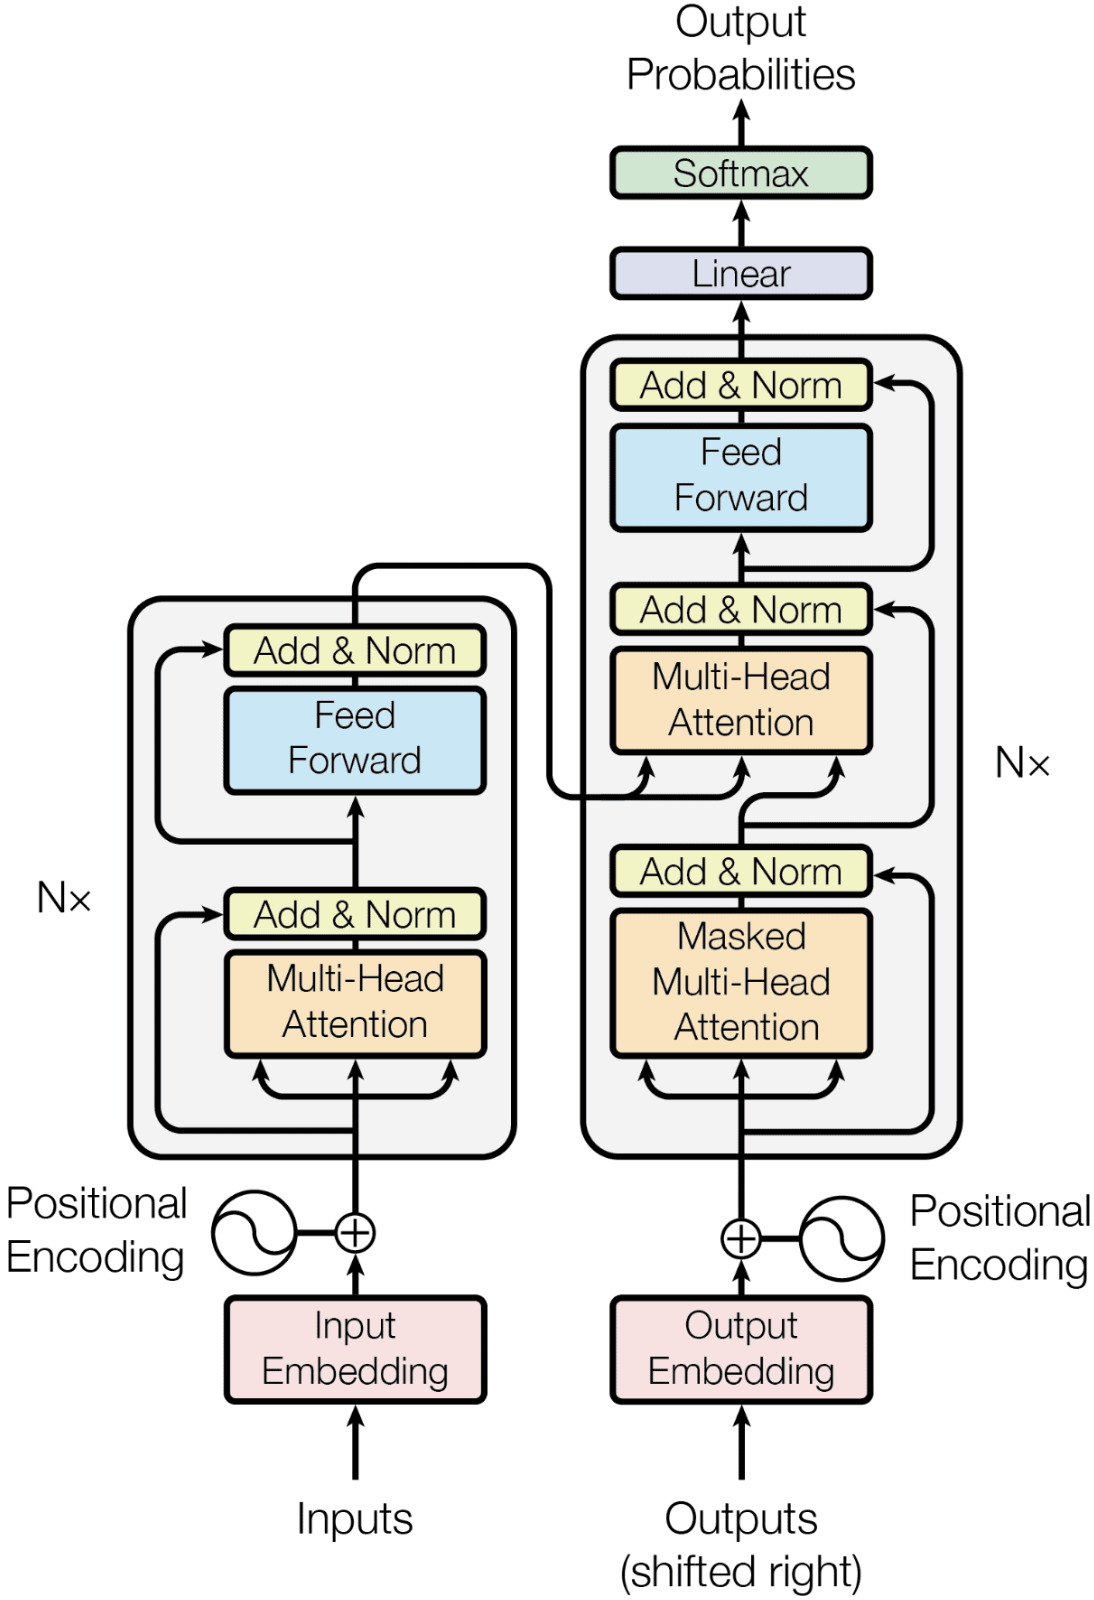
\includegraphics[width=0.5\linewidth]{img/transformer_arch.png}
\caption{Transformer model architecture \cite{arxiv-attention}.}
\label{fig:transformer}
\end{figure}

The figure above shows the original architecture of a Transformer model, as presented in the paper \textit{``Attention Is All You Need''} \cite{arxiv-attention}, comprising all its internal components.
The operation of each of these components is explained below.

%%% Correggere insieme a tutte le volte che dici tokenization
\subsection{Input Representation}
The textual input sequence requires a preprocessing phase to be converted into a compatible numerical format \cite{stanford}. This process consists of three main stages:
\begin{itemize}
\item \textbf{Tokenization} \cite{stanford}
\item \textbf{Input Embedding} \cite{arxiv-attention}
\item \textbf{Positional Encoding} \cite{arxiv-attention, Muhammad_Faizan}
\end{itemize}
These three phases are described below.

\paragraph{Tokenization}
In this first phase, the input sequence—assumed to be textual for simplicity—is divided into multiple sub-sequences called tokens \cite{stanford, git-hub}. Each token belongs to a finite set of strings called the vocabulary $V$ \cite{stanford}. Each token is assigned an integer numerical value corresponding to the position it occupies in the vocabulary \cite{git-hub}.

\begin{figure}[H]
\centering
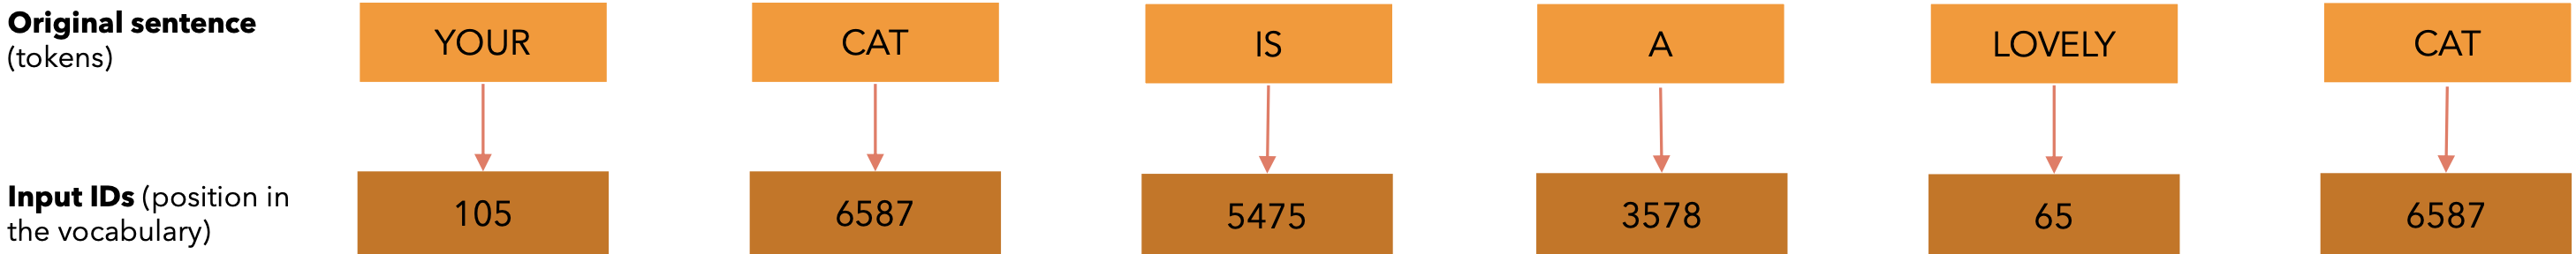
\includegraphics[width=1\linewidth]{img/tokenization.png}
\caption{Representation of the Tokenization phase on the text sequence \textit{"your cat is a lovely cat"} \cite{git-hub}. The input sequence is split into tokens, in this case represented by each word, which are then associated with the corresponding integer in the vocabulary $V$.}
\label{fig:tokenization} % Ho cambiato l'etichetta da placeholder per unicità
\end{figure}

\paragraph{Input Embedding} The numerical values obtained through tokenization are then mapped as vectors of dimension $d_{model}=512$ \cite{arxiv-attention}; every value contained in these vectors is learned during training \cite{git-hub, stanford}. Following these steps, the input text sequence is converted into a series of vectors of $d_{model}$ learned elements called embeddings \cite{arxiv-attention, stanford}.

\begin{figure}[H]
\centering
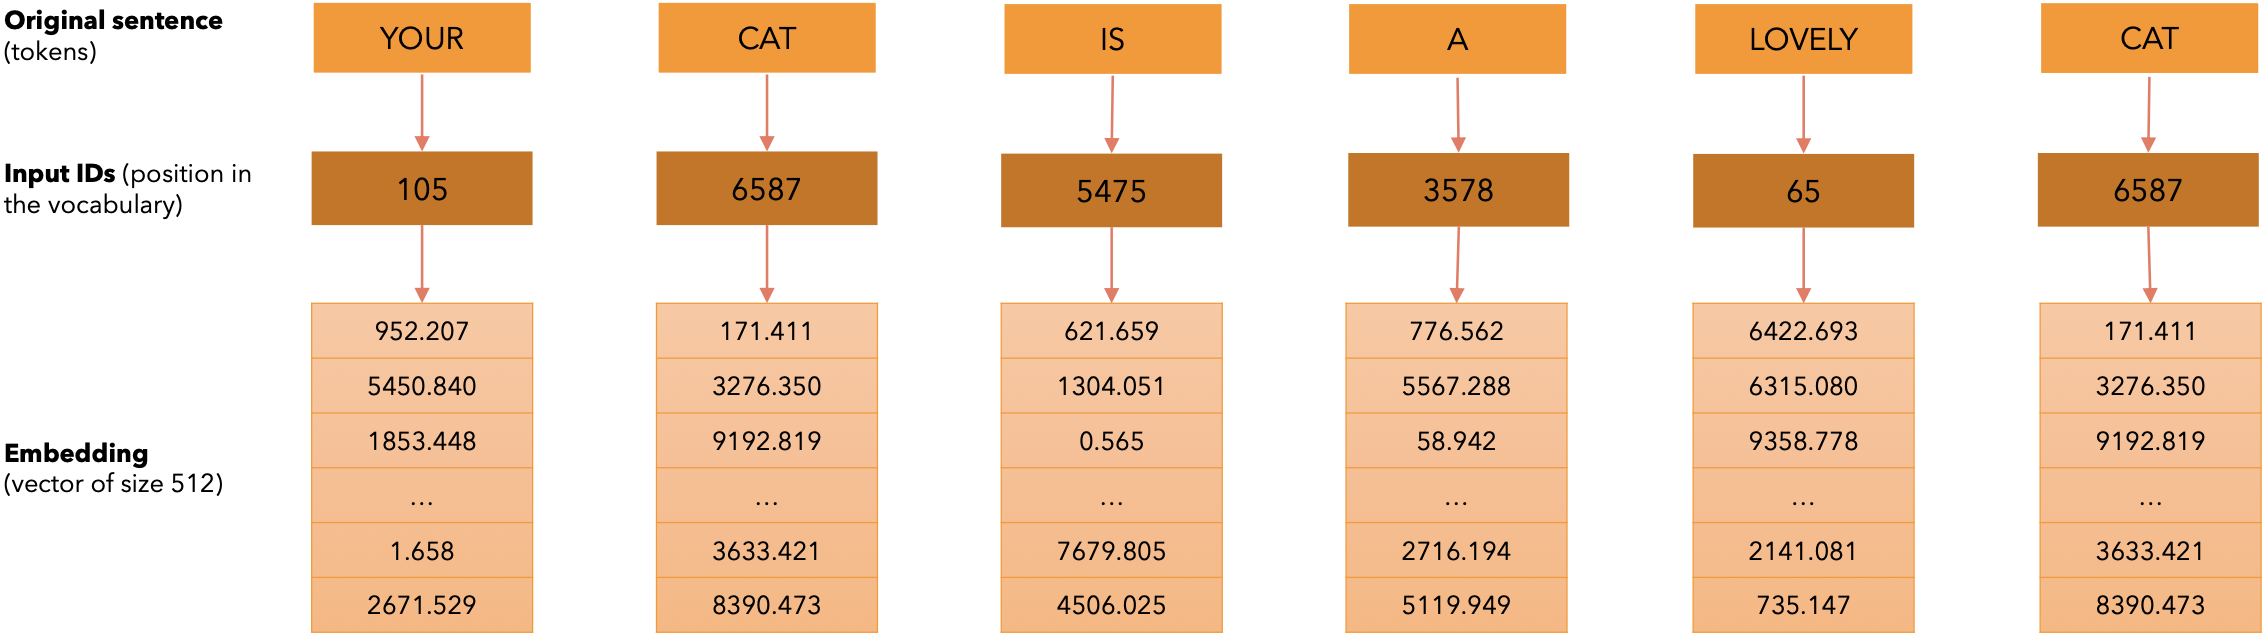
\includegraphics[width=1\linewidth]{img/input_embedding_2.png}
\caption{Representation of the Input Embedding phase \cite{git-hub}.}
\label{fig:embedding}
\end{figure}

\paragraph{Positional Encoding} With the aim of providing order information, each embedding is added to a positional vector $p_{pos} \in \mathbb{R}^{d_{model}}$ \cite{arxiv-attention, Muhammad_Faizan}. 

Each positional vector is calculated as \cite{arxiv-attention}:
\begin{equation}
PE(pos, 2i) = \sin \left(\frac{pos}{10000^{\frac{2i}{d_{model}}}}\right) \quad \textbf{for even \textit{i}}
\end{equation}

\begin{equation}
 PE(pos, 2i+1) = \cos \left(\frac{pos}{10000^{\frac{2i}{d_{model}}}}\right) \quad \textbf{for odd \textit{i}}
\end{equation}

where \cite{Muhammad_Faizan, git-hub}:
\begin{itemize}
\item $pos$ represents the index of the position vector within the sequence
\item $i$ represents the position of the element within the vector $pos$
\end{itemize}

\begin{figure}[H]
\centering
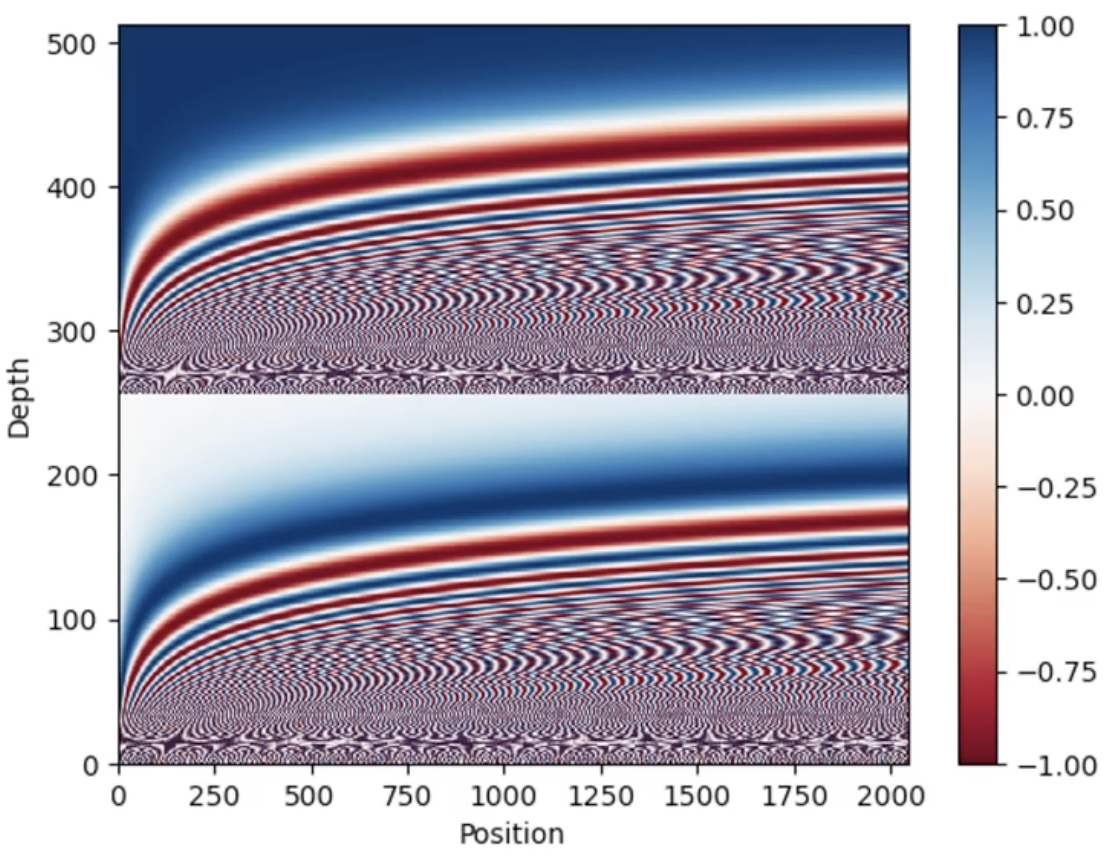
\includegraphics[width=0.5\linewidth]{img/positional_encoding_graphic.png}
\caption{Visualization of the sinusoidal positional encoding matrix for a model with $d_{model}=512$ \cite{git-hub}. The horizontal axis represents the token position in the sequence, while the vertical axis indicates the encoding vector dimension \cite{git-hub}. The color encodes the value of the sine function, which ranges from -1 to +1 \cite{Muhammad_Faizan, git-hub}.}
\label{fig:pos_encoding}
\end{figure}

The sine and cosine functions were chosen for positional encoding calculation because they offer a combination of properties ideal for representing order in a non-recurrent architecture \cite{arxiv-attention, Muhammad_Faizan}:
\begin{itemize}
\item \textbf{Positional Uniqueness:} Each position in the sequence has a unique positional encoding vector \cite{Muhammad_Faizan}. The combination of sine waves at different frequencies (controlled by the term $10000^\frac{2i}{d_{model}}$) ensures that no two positions share the exact same encoding vector \cite{arxiv-attention}.
\item \textbf{Relative Position Representation:} For a fixed distance $k$, the encoding vector at position $pos + k$ can be represented as a linear transformation of the vector at position $pos$ \cite{arxiv-attention}. This allows the model to easily learn to recognize relative positions, independently of the absolute position \cite{Muhammad_Faizan}. The attention mechanism, being based on dot products (a linear transformation), can directly leverage this property \cite{git-hub}.
\item \textbf{Generalization to Longer Sequences:} Since sine and cosine functions are periodic and their behavior is well-defined outside the training interval, the model can extrapolate to sequences longer than those seen during training \cite{arxiv-attention, Muhammad_Faizan}.
\item \textbf{Bounded Values and Stability:} Sine and cosine values are naturally bounded within the interval $\left[-1,1\right]$, which helps keep embedding values normalized and contributes to numerical stability during training \cite{Muhammad_Faizan}.
\end{itemize}
The positional embeddings are then added to the corresponding embeddings \cite{arxiv-attention}.
The result of this operation constitutes the input to the Encoder \cite{git-hub, stanford}.

\begin{figure}[H]
\centering
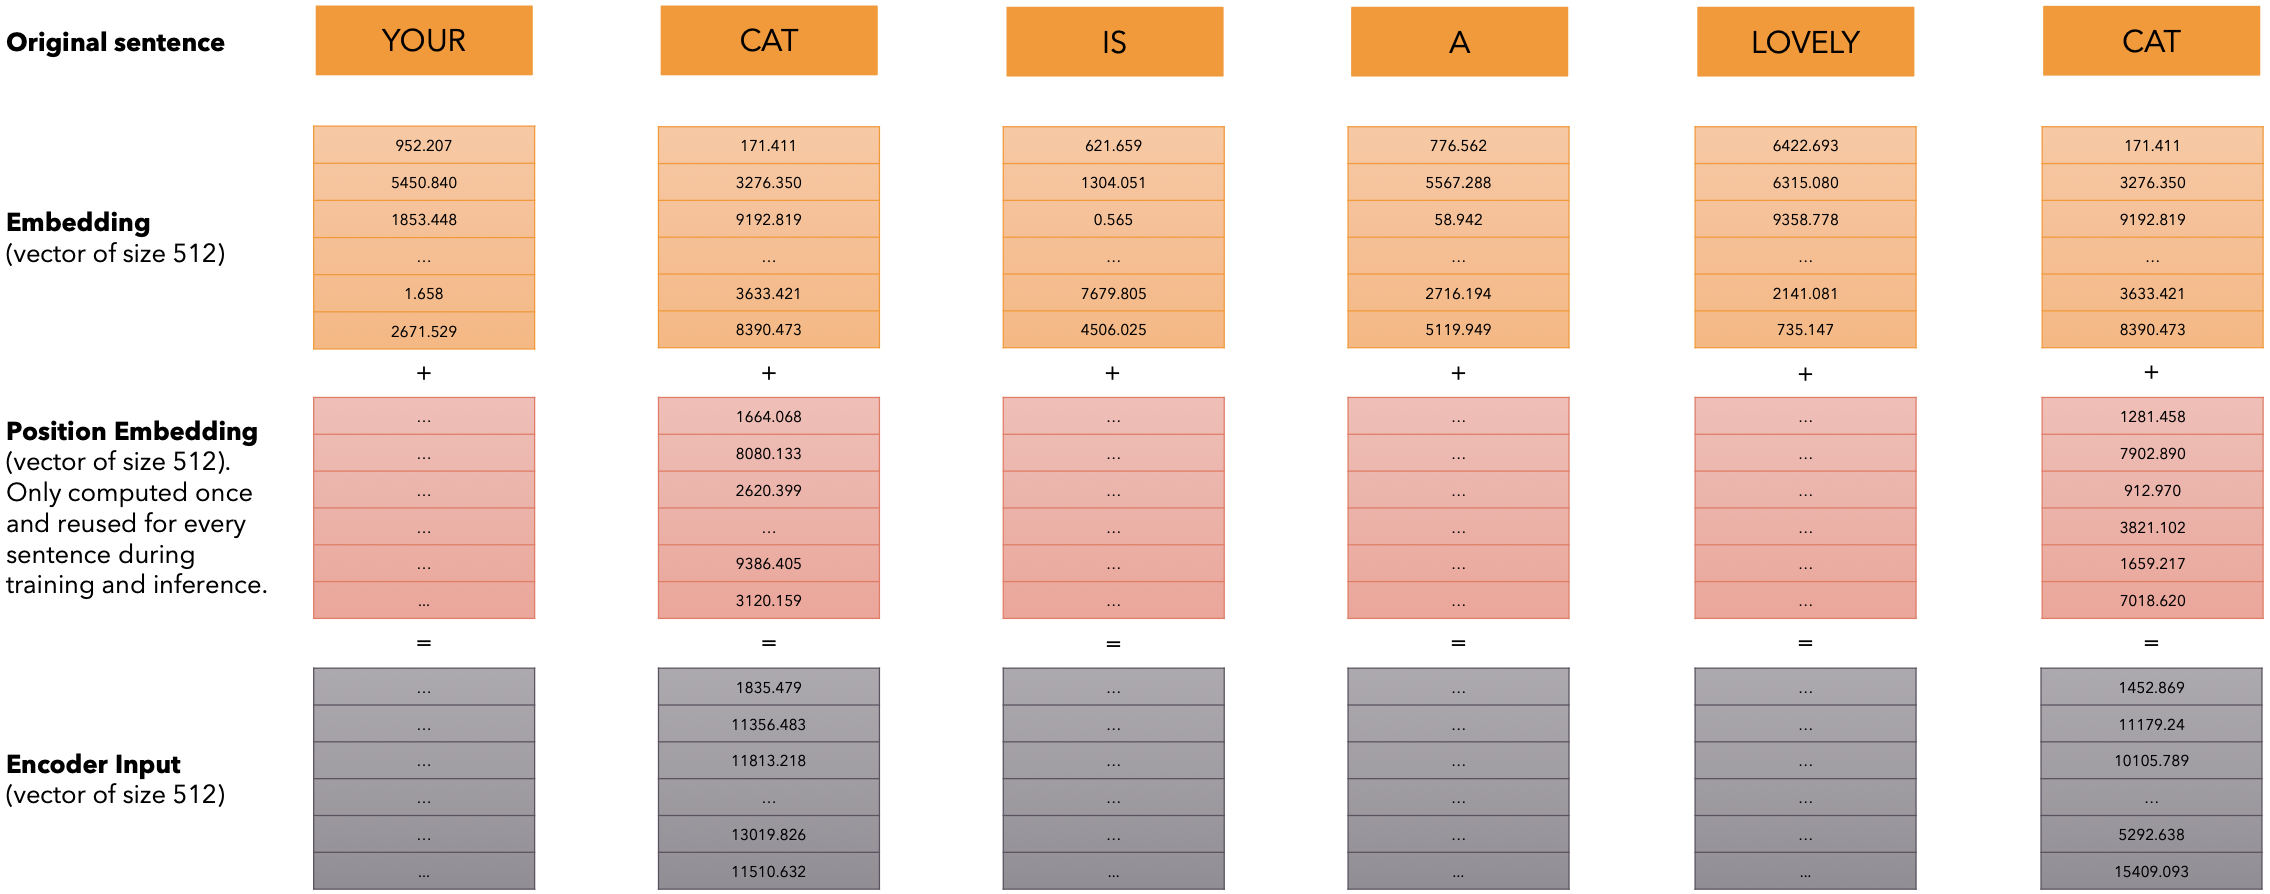
\includegraphics[width=1\linewidth]{img/tokenization_summary.png}
\caption{Summary scheme of Input Representation via Tokenization, Input Embedding, and Positional Encoding \cite{git-hub}.}
\label{fig:input_summary}
\end{figure}

\subsection{Self-Attention}
The fundamental component of the Transformer architecture is the self-attention mechanism \cite{arxiv-attention, stanford}. Unlike recurrent models that process sequences serially, self-attention allows the model to weigh the importance of each token within a sequence in relation to all others, capturing contextual dependencies independently of their distance \cite{arxiv-attention, GeeksForGeeks}. 

The computation of self-attention, considered here as single-head, is based on a function called Scaled Dot-Product Attention \cite{arxiv-attention}. Formally, the input to this mechanism consists of three matrices \cite{arxiv-attention, hashnode}:
\begin{itemize}
\item \textbf{Query Matrix} $\rightarrow \quad Q \in \mathbb{R}^{seq \times d_{k} }$ 
\item \textbf{Key Matrix} $\rightarrow \quad K \in \mathbb{R}^{seq \times d_{k} }$
\item \textbf{Value Matrix} $\rightarrow \quad V \in \mathbb{R}^{seq \times d_{v} }$
\end{itemize}
Where \cite{arxiv-attention, git-hub}:
\begin{itemize}
\item $seq$ represents the length of the input sequence
\item $d_k, d_v$ are the dimensions of the representations
\end{itemize}
These three matrices are obtained by projecting the input matrix $ X \in \mathbb{R}^{seq \times d_{model}}$, constructed by stacking the input representation vectors, via three distinct weight matrices $W^Q \in \mathbb{R}^{d_{model} \times d_{k}}, W^K\in \mathbb{R}^{d_{model} \times d_{k}}$, and $W^V\in \mathbb{R}^{d_{model} \times d_{v}}$ learned during training \cite{arxiv-attention, hashnode, stanford}:
\begin{equation}
Q=XW^Q, \quad K= XW^K,\quad V=XW^V 
\end{equation}

The Scaled Dot-Product Attention function is then calculated as follows \cite{arxiv-attention}:
\begin{equation}
Attention(Q, K, V)=softmax\left(\frac{QK^T}{\sqrt{d_k}}\right)V
\end{equation}

This operation produces the so-called attention matrix \cite{arxiv-attention, hashnode}. \footnote{The scaling factor $\frac{1}{\sqrt{d_k}}$ is crucial \cite{arxiv-attention}. Without it, for large values of $d_k$, the dot products can grow large in magnitude, pushing the softmax function into regions where it has extremely small gradients (vanishing gradients) \cite{git-hub, arxiv-attention}. This would effectively halt the training process \cite{arxiv-attention}.}
\begin{figure}[H]
\centering
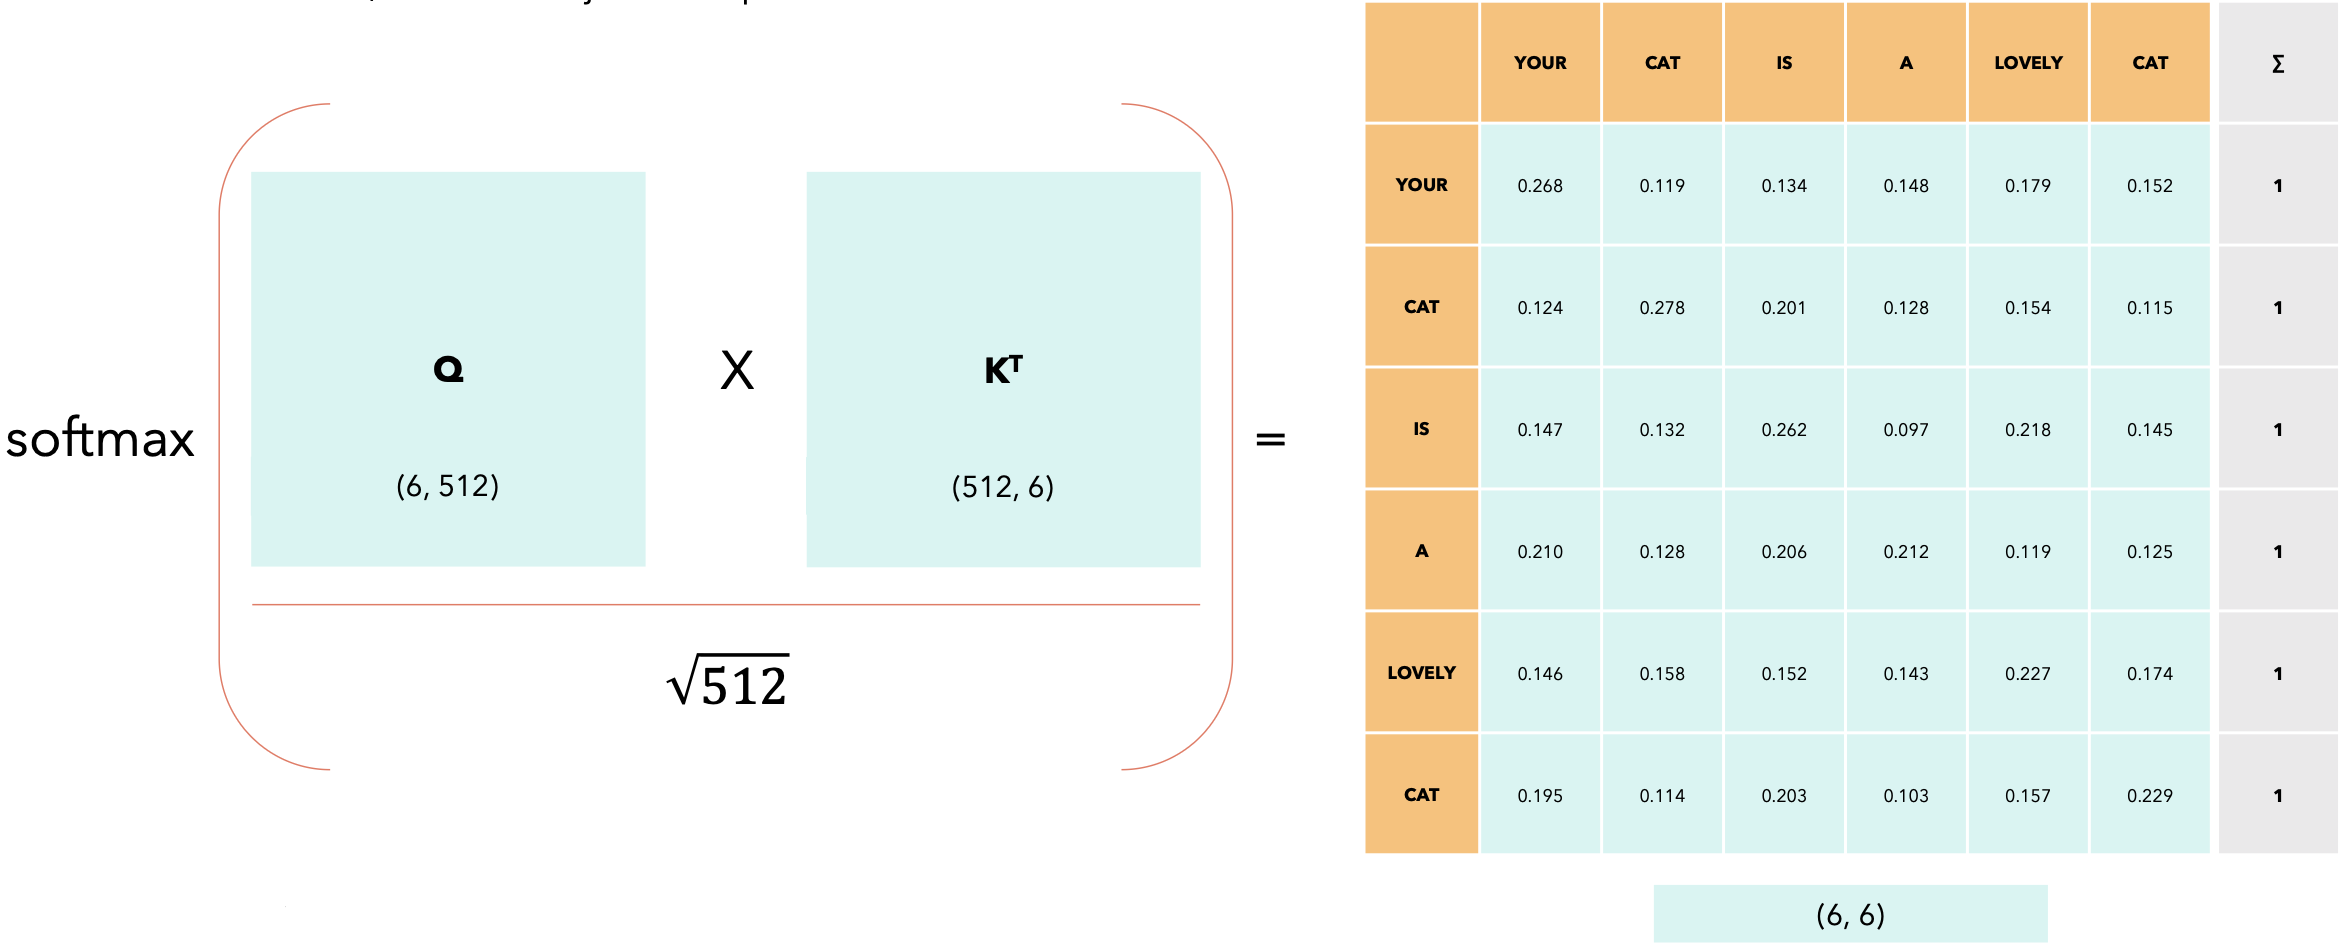
\includegraphics[width=1\linewidth]{img/self_attention.png}
\caption{Softmax of the Scaled Dot-Product Attention calculated by setting, for simplicity, $d_k=d_v=d_{model}=512$, $seq=6$, and following the previous examples \cite{git-hub}. Note how, thanks to the \textit{softmax}, the sum of each row is 1.}
\label{fig:self_attention_softmax}
\end{figure}

\begin{figure}[H]
\centering
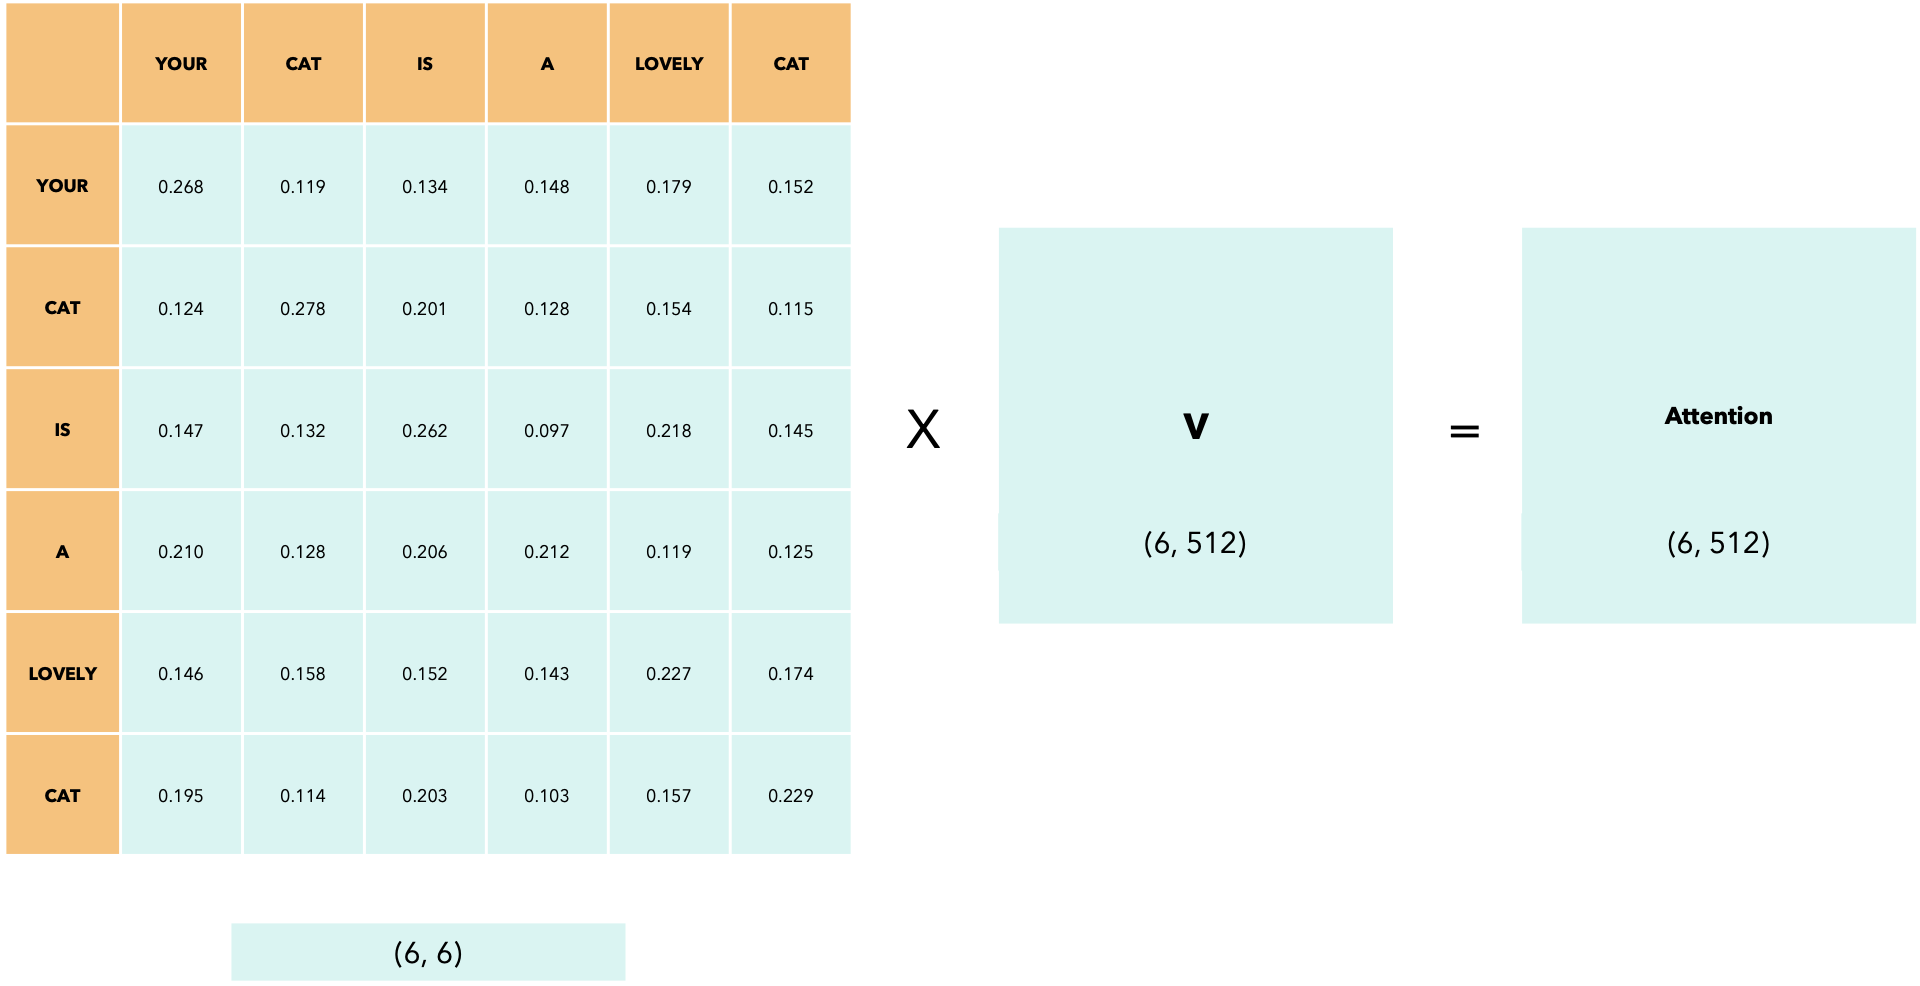
\includegraphics[width=1\linewidth]{img/self_attention_result.png}
\caption{Result of the Scaled Dot-Product Attention introduced in the previous figure. Each row of the resulting attention matrix will capture not only the meaning (thanks to the embedding) and the position in the sequence (thanks to the positional encoding) but also every interaction of each token with the other tokens \cite{git-hub}.}
\label{fig:self_attention_result}
\end{figure}

\subsubsection{In-depth Analysis of Q, K, and V Matrices}
The Query, Key, and Value matrices play distinct and complementary roles in the attention calculation process, allowing the model to effectively weigh the importance of each token in the sequence relative to the others \cite{arxiv-attention, stanford, git-hub}.
To better understand the role of the individual matrices, an analogy can be used \cite{hashnode, GeeksForGeeks}: \textit{Imagine being in a library and wanting to find books on a particular topic.}
We can structure the situation as follows:
\begin{itemize}
\item \textbf{Query (Q):} Represents the question we ask. For example: \textit{"I am looking for books on Renaissance art history."} The query encodes what we are looking for, the important features in our case.
\item \textbf{Key (K):} Represents the labels or cataloging of the books. Each book has metadata stating: \textit{"This book is about: history, art, Renaissance, France, 1500."} The keys make the books "searchable."
\item \textbf{Value (V):} Represents the actual content of the books. Once we find the books that match our searches, i.e., with \textbf{high similarity between Q and K}, we retrieve their content to read and understand.
\end{itemize}

We can therefore describe, more formally, the semantic role of each of these three matrices.

\paragraph{Semantic Role of the Query} The Query represents, as mentioned, the "question" that each token poses to the rest of the sequence \cite{arxiv-attention, stanford}. Concretely, the query vector $q_i=x_iW^Q$ of a token $i$ encodes what information that token is seeking from other words in the sequence to better understand its own meaning within the context \cite{hashnode, GeeksForGeeks}. For example, in a sentence like \textit{"The cat meows"}, the token \textit{"cat"} might have a query that "looks for" information about actions it performs (represented by the key of \textit{"meows"}) or determinants that qualify it (represented by the key of \textit{"The"}).
Formally, during the attention calculation, the query of token $i$ is compared with the keys of all tokens via the dot product, thus measuring the compatibility between what token $i$ is looking for and what the other tokens offer \cite{arxiv-attention, git-hub}.

\paragraph{Semantic Role of the Key} The Key represents the "search labels" or "identifying metadata" of each token \cite{hashnode, GeeksForGeeks}. The key vector $k_j=x_jW^K$ of a token $j$ encodes which characteristics make that token identifiable and searchable by tokens seeking information \cite{arxiv-attention}. The key of a token exposes the salient traits that distinguish it and make it relevant in different contexts. The role of the key is crucial in determining relevance: every query of every token is compared (via dot product) with the key of every other token \cite{arxiv-attention, stanford}. A high value of $q_i \cdot k_j$ indicates that token $j$ contains information that token $i$ is looking for, and therefore deserves a high attention weight \cite{git-hub}.

\paragraph{Semantic Role of the Value} The Value represents the actual semantic content that each token contributes to the contextualized representation of the other tokens \cite{arxiv-attention, stanford}. The value vector $v_j=x_jW^V$ of a token $j$ encodes the intrinsic meaning of the token, suitably transformed to be combinable with the values of other tokens \cite{hashnode, GeeksForGeeks}.

Unlike Query and Key, which are used to calculate attention weights, the Value is combined according to these weights \cite{arxiv-attention}. By decomposing the Scaled Dot-Product Attention into two phases:
\begin{equation*}
    AttentionWeights=softmax\left( \frac{QK^T}{\sqrt{d_k}} \right) \quad \tag{Phase 1}
\end{equation*}
where $AttentionWeights$ results in a matrix in $\mathbb{R}^{seq\times seq}$ containing the attention weights \cite{arxiv-attention, git-hub}. The element $(i,j)$ of this matrix therefore indicates how much token $i$ should attend to element $j$ of the sequence.

\begin{equation*}
Attention=AttentionWeights\cdot V \tag{Phase 2}
\end{equation*}
where $Attention \in \mathbb{R}^{seq \times d_V}$ contains the final output of the attention mechanism, in which each row $z_i$ represents token $i$ contextualized within the input sequence \cite{arxiv-attention}.

The contextualized representation of each single token is therefore obtained as a weighted sum of all the value vectors of the sequence \cite{stanford, git-hub}:
\begin{equation}
z_i=\sum^n_{j=1}AttentionWeights_{ij}\cdot v_j
\end{equation}

\subsubsection{Properties of the Self-Attention Mechanism}
The characteristics of Self-Attention include:
\begin{itemize}
\item \textbf{Permutation Equivariance:} A function $f:\mathbb{R}^{n\times d} \rightarrow \mathbb{R}^{n\times d}$ is permutation equivariant if, for any input matrix $X \in \mathbb{R}^{n\times d}$ and any permutation matrix $P_\pi \in \mathbb{R}^{d\times d}$ (which permutes the rows of $X$), the following holds \cite{arxiv-permutation-equivariance-transformers}:
\begin{equation}
f(P_\pi X) = P_\pi f(X)
\end{equation}
This implies that if the rows of the input matrix $X$ are permuted, the rows of the output attention matrix will be permuted in the same manner \cite{arxiv-permutation-equivariance-transformers, git-hub}.

Although this property ensures that the model does not arbitrarily favor specific positions in the sequence, it presents a critical aspect: without further mechanisms, the model would be insensitive to the sequence order \cite{arxiv-permutation-equivariance-transformers}. Two identical sequences in different orders—for example, \textit{"Riccardo greets Alice"} and \textit{"Alice greets Riccardo"}—would produce numerically equivalent (albeit permuted) outputs \cite{arxiv-permutation-equivariance-transformers}. To address this issue, the Transformer introduces positional encoding, which adds explicit positional information to each token \cite{arxiv-permutation-equivariance-transformers, git-hub, arxiv-attention}, effectively breaking permutation equivariance and allowing the model to capture and represent dependencies related to the sequence order \cite{arxiv-permutation-equivariance-transformers}.

\item \textbf{Long-Range Dependency Modeling:} Unlike recurrent networks, where information must traverse all intermediate steps sequentially, self-attention reduces the maximum signal path length to a constant value of $O(1)$ \cite{arxiv-attention, stanford}. This allows for directly connecting every pair of tokens regardless of their positional distance, facilitating the learning of global semantic relationships \cite{arxiv-attention, GeeksForGeeks}.

\item \textbf{Full Parallelizability:} In contrast to Recurrent Neural Networks (RNNs), self-attention consists exclusively of matrix multiplications, allowing for total parallelization on \textit{GPUs} \cite{arxiv-attention, git-hub}.

\item \textbf{Computational Complexity:} It has a time complexity of $O(seq^2d_{model})$ and a memory complexity of $O(seq^2)$ \cite{arxiv-attention, arxiv-attention, stanford}, \footnote{This quadratic complexity represents a significant bottleneck in the medical domain, where inputs such as Electronic Health Records (EHRs) or genomic sequences can be extremely long \cite{pmc-timelygpt}. This limitation has led to the development of "efficient Transformers" (e.g., Longformer, BigBird) specifically designed to handle long contexts with linear or log-linear complexity \cite{arxiv-efficient-transformers}.} making it efficient for sequences of moderate length but prohibitive for very long sequences \cite{arxiv-attention}.

\item \textbf{Differentiability:} All components are differentiable, allowing training via backpropagation without non-derivable components \cite{arxiv-attention, git-hub}.
\end{itemize}

\subsection{Multi-head Attention}
The self-attention mechanism, described in the previous section, computes a single contextualized representation for each token via a single attention operation. However, this architecture limits the model's ability to simultaneously capture different types of relationships between tokens \cite{arxiv-attention, stanford, git-hub}. For instance, the model might need to identify grammatical agreements (where a verb should attend to the subject), positional proximity relationships, or semantic similarities, all concurrently \cite{GeeksForGeeks}. A single linear transformation cannot effectively represent all these dimensions of meaning simultaneously \cite{git-hub}. The solution proposed in the paper \textit{"Attention Is All You Need"} is the Multi-Head Attention mechanism, which allows the model to perform attention calculations in parallel \cite{arxiv-attention}. Each attention "head" learns to specialize in extracting a different type of contextual relationship, and the outputs of all heads are subsequently combined \cite{arxiv-attention, stanford}.
\begin{figure}[H]
\centering
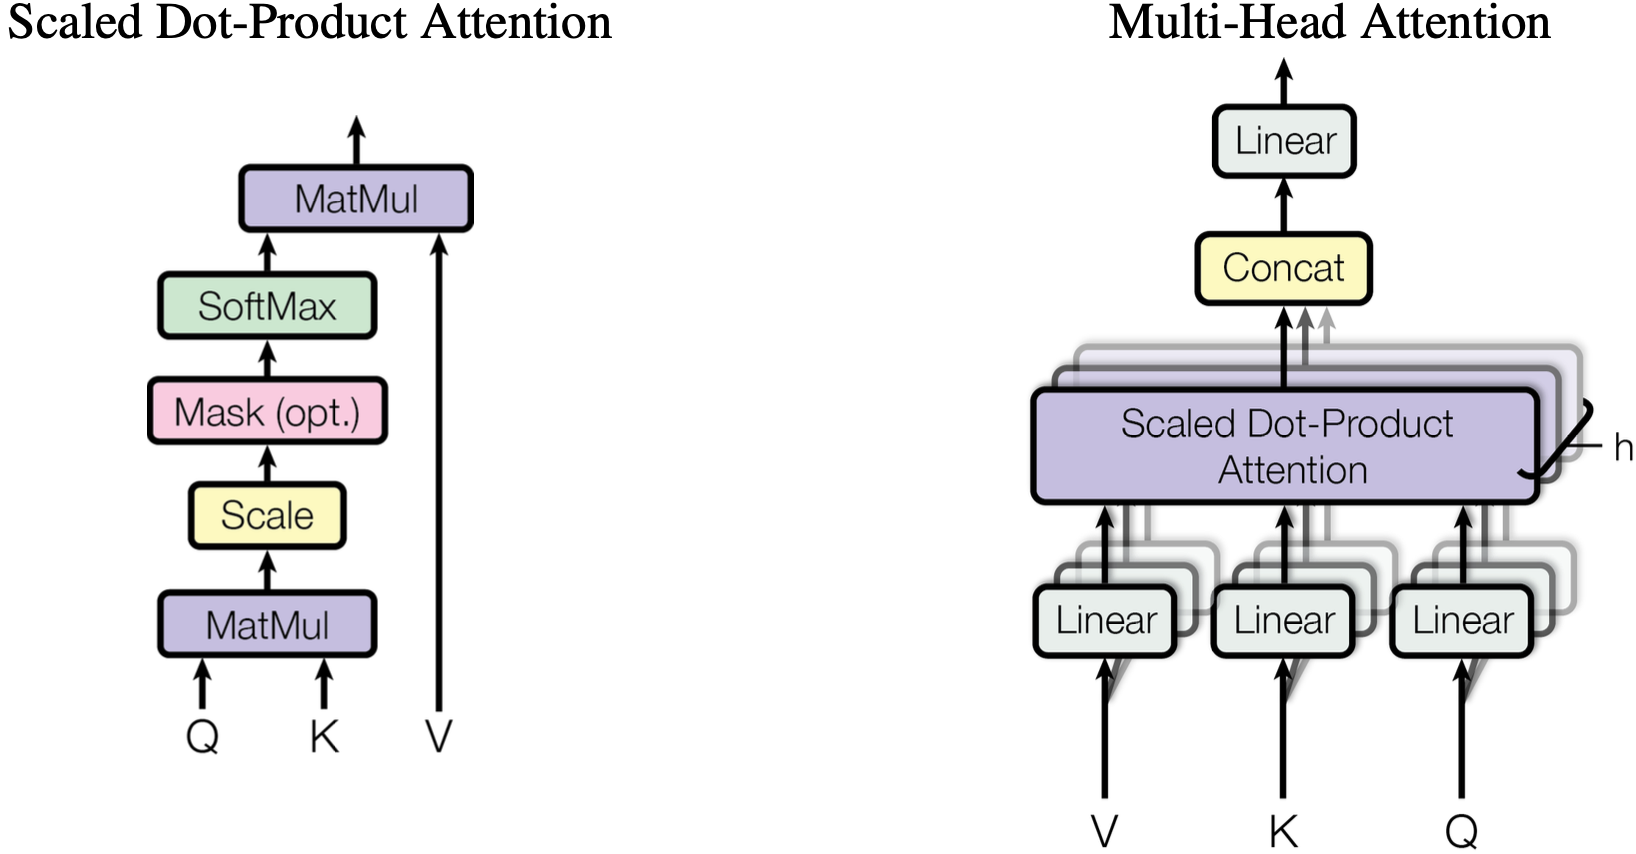
\includegraphics[width=1\linewidth]{img/multi-and-single-head.png}
\caption{On the left is a schematic representation of Scaled Dot-Product Attention (single-head) \cite{arxiv-attention}. On the right is a schematic representation of Multi-Head Attention consisting of several Attention layers in parallel \cite{arxiv-attention}.}
\label{fig:scaled_dot}
\end{figure}

\subsubsection{Hyperparameter Specification}
Let $h$ be the number of attention heads (a hyperparameter, typically 8 or 16 in standard models) \cite{arxiv-attention, stanford}. In the original paper, to ensure the computational cost remains manageable, the dimensions are set as \cite{arxiv-attention}:
\begin{equation}
d_k=d_v=\frac{d_{model}}{h}
\end{equation}

For each head $i\in\{1, 2, \dots, h\}$, three independent weight matrices are defined, which are learned during training \cite{arxiv-attention, git-hub}:
$$
W^Q_i\in \mathbb{R}^{d_{model}\times d_k}, W^K_i\in \mathbb{R}^{d_{model}\times d_k}, W^V_i\in \mathbb{R}^{d_{model}\times d_v}
$$
Additionally, a final output weight matrix \cite{arxiv-attention}:
$$
W^O \in \mathbb{R}^{(h\cdot d_v)\times d_{model}}
$$

\subsubsection{Operational Flow}
\paragraph{Linear Projections per Head}
The input matrix $X \in \mathbb{R}^{seq\times d_{model}}$, produced by tokenization, is projected into Query, Key, and Value for each head $i=\{1,\dots,h\}$ \cite{arxiv-attention, stanford}:
\begin{equation}
Q_i=XW^Q_i, K_i=XW^K_i, V_i=XW^V_i
\end{equation}

where:
\begin{itemize}
\item $Q_i=XW^Q_i \in \mathbb{R}^{seq\times d_{k}},$ represents the Query matrix corresponding to head $i$
\item $K_i=XW^K_i \in \mathbb{R}^{seq\times d_{k}},$ represents the Key matrix corresponding to head $i$
\item $V_i=XW^V_i \in \mathbb{R}^{seq\times d_{v}},$ represents the Value matrix corresponding to head $i$
\end{itemize}
This operation will therefore yield a set of $h$ distinct Query, Key, and Value matrices \cite{arxiv-attention, git-hub}. \footnote{From an implementation perspective (e.g., in frameworks like PyTorch \cite{pytorch-multiheadattention} or TensorFlow \cite{tensorflow-multiheadattention}), these projections are rarely performed as a loop over $h$ separate matrices \cite{stanford}. Instead, a single large weight matrix (of size $d_{model} \times d_{model}$) is used to project the input at once, and the resulting tensor is subsequently reshaped to separate the heads \cite{stanford, git-hub}. This "vectorized" approach leverages GPU parallelism to maximize efficiency, while producing a mathematically equivalent result to the separate formulation \cite{stanford}. The figures in this section illustrate this efficient implementation strategy (labeled as \textit{"Alternative Approach"}) \cite{git-hub, stanford}.}

Since each head possesses distinct weight matrices, the input is "viewed" from multiple different perspectives, allowing for the extraction of different semantic structures from the input \cite{arxiv-attention, stanford, git-hub}.
\begin{figure}[H]
\centering
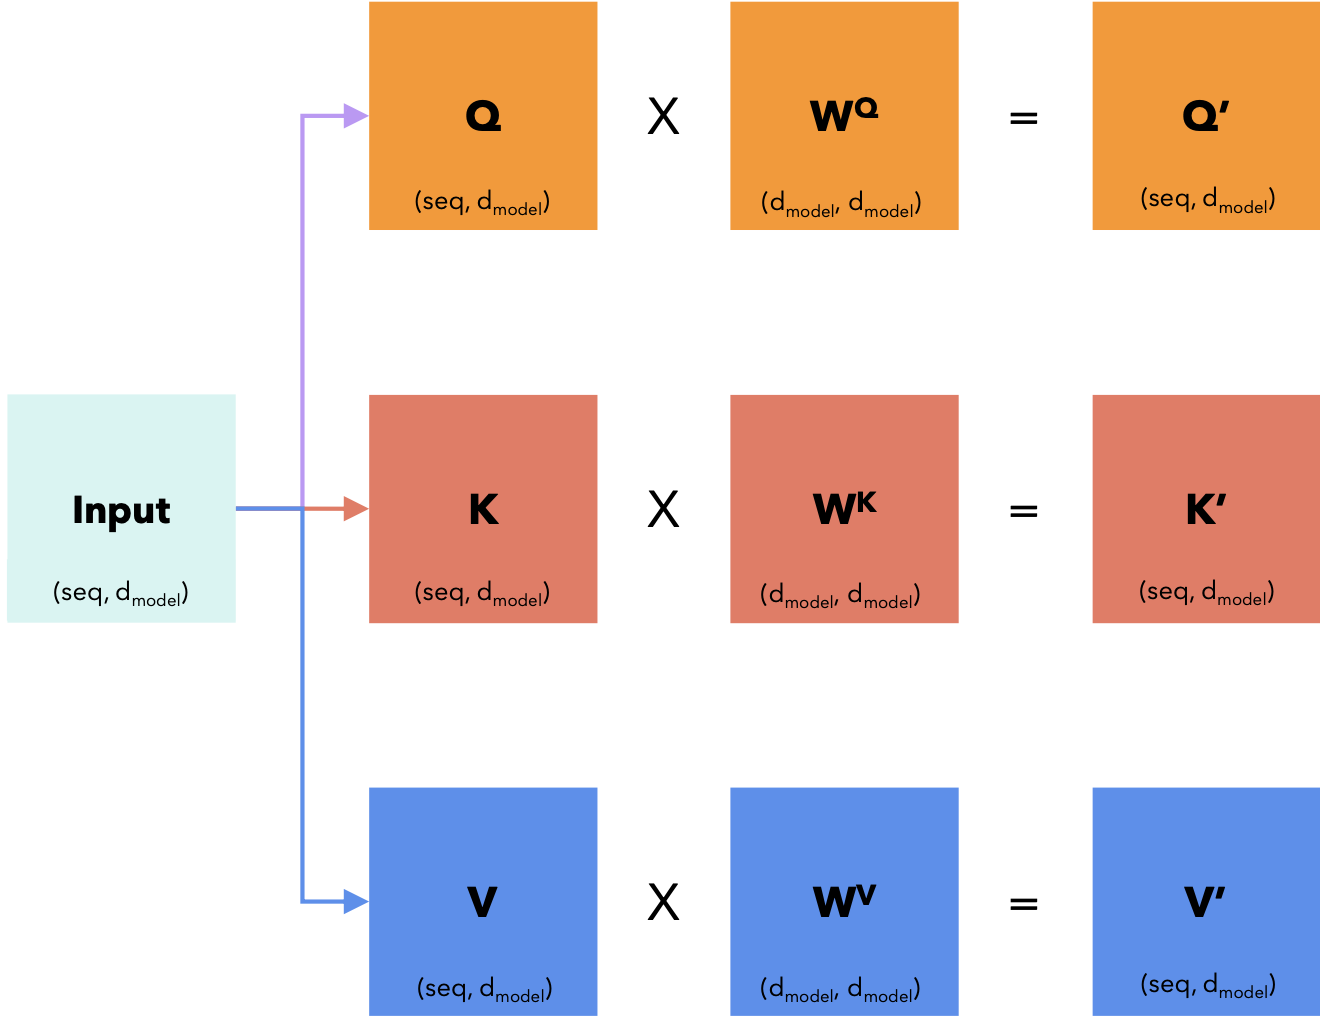
\includegraphics[width=0.8\linewidth]{img/Proiezioni_Lineari_mh.png}
\caption{\textbf{(Alternative Approach, \textit{Step 1})} Graphical representation of the linear projection calculation for $Q, K$, and $V$ \cite{git-hub}. In this case, for efficiency reasons, three matrices $W$ of dimension $d_{model}\times d_{model}$ (thus larger) are considered and projected a single time onto $K, V$, and $Q$. The matrices resulting from this operation, $Q', K'$, and $V'$ of dimension $seq \times d_{model}$, are then split into $h$ matrices that will constitute the heads.}
\label{fig:mh_step1}
\end{figure}

\paragraph{Self-Attention Calculation for Each Head}
The Scaled Dot-Product Attention mechanism is applied independently to each head in parallel \cite{arxiv-attention, stanford}:
\begin{equation}
head_i=Attention(Q_i, K_i, V_i)=Softmax\left( \frac{Q_iK_i^T}{\sqrt{d_k}}\right)V_i
\end{equation}

Each triplet of matrices $(Q_i, K_i, V_i)$ produces an output matrix $head_i\in\mathbb{R}^{seq\times d_v}$ \cite{arxiv-attention}. The result of this operation will therefore consist of $h$ distinct head matrices \cite{git-hub}.
\begin{figure}[H]
\centering
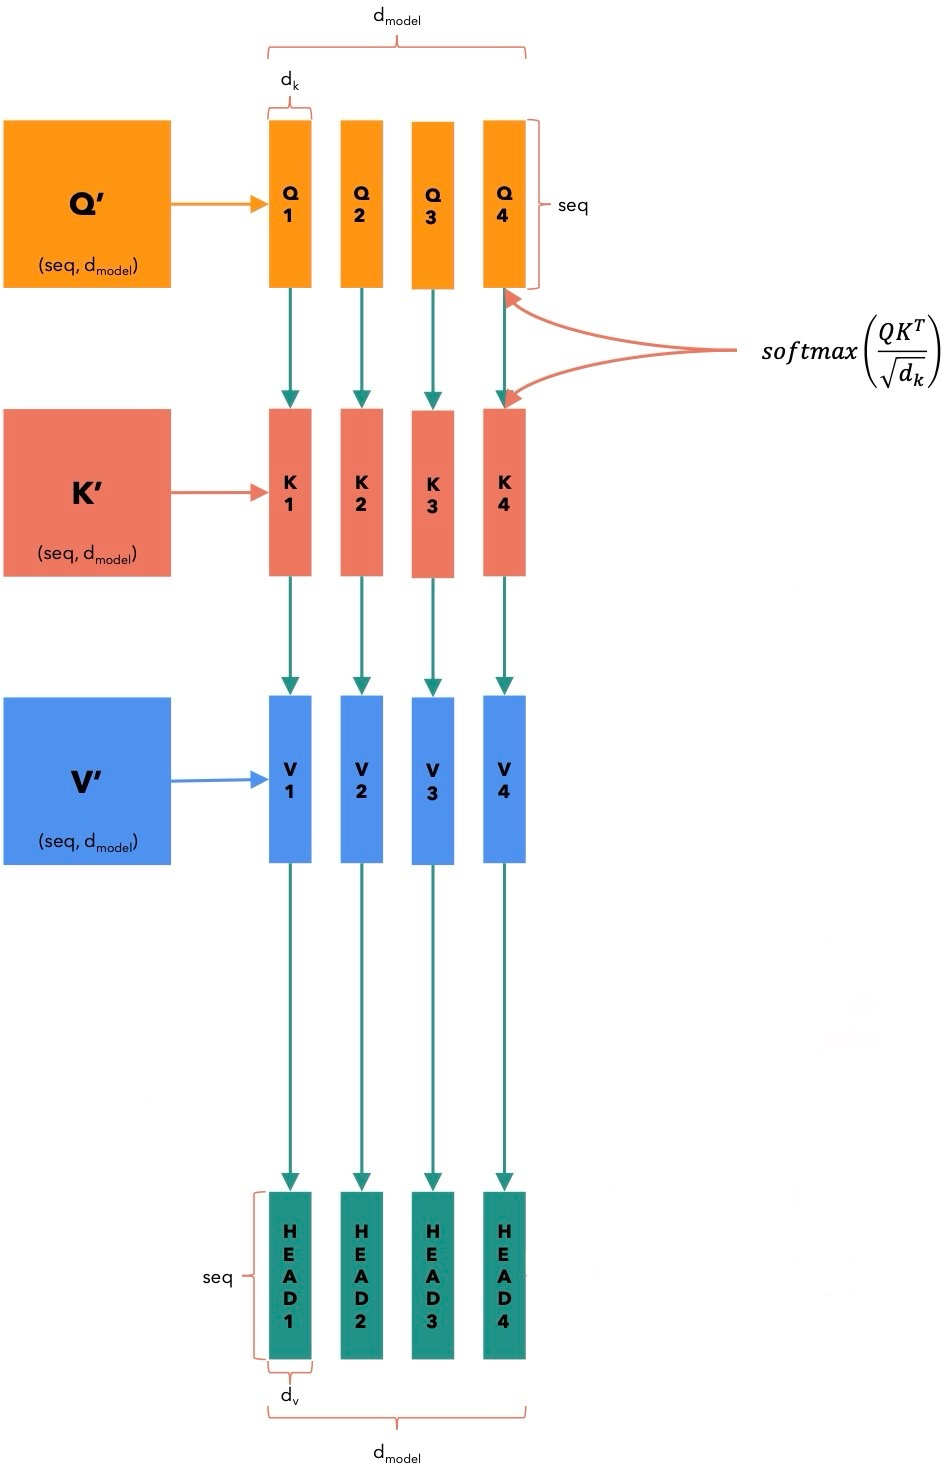
\includegraphics[width=0.8\linewidth]{img/mh-step-2.jpeg}
\caption{\textbf{(Alternative Approach, \textit{Step 2})} In this case, the matrices $Q', K'$, and $V'$, obtained in the previous step, are split into $h$ matrices of size $seq\times d_k$ \cite{git-hub}. Dot-Product Attention is then calculated on each triplet of sub-matrices $(Q_1,K_1,V_1), \dots, (Q_h, K_h, V_h)$. The result of this operation will consist of $h$ head matrices with $head_i \in \mathbb{R}^{seq\times d_v}$.}
\label{fig:mh_step2}
\end{figure}

\paragraph{Concatenation of Head Outputs}
In this phase, the $h$ heads, just computed, are concatenated along axis \textit{1} to produce a single matrix of size $seq\times d_{model}$ \cite{arxiv-attention, stanford}:
\begin{equation}
Concat=[head_1 \oplus head_2 \oplus \dots\oplus head_h] \in \mathbb{R}^{seq\times (h \cdot d_{v})}
\end{equation}

where:
\begin{itemize}
\item $\oplus$ represents concatenation along axis \textit{1} \cite{git-hub}
\end{itemize}
Note how the dimension of the concatenation matrix $Concat$, in this case, is equivalent to $seq\times d_{model}$ \cite{arxiv-attention}:
$$
seq\times (h\cdot d_v) = seq \times \left(h \cdot \frac{d_{model}}{h}\right) = seq \times d_{model}
$$
\begin{figure}[H]
\centering
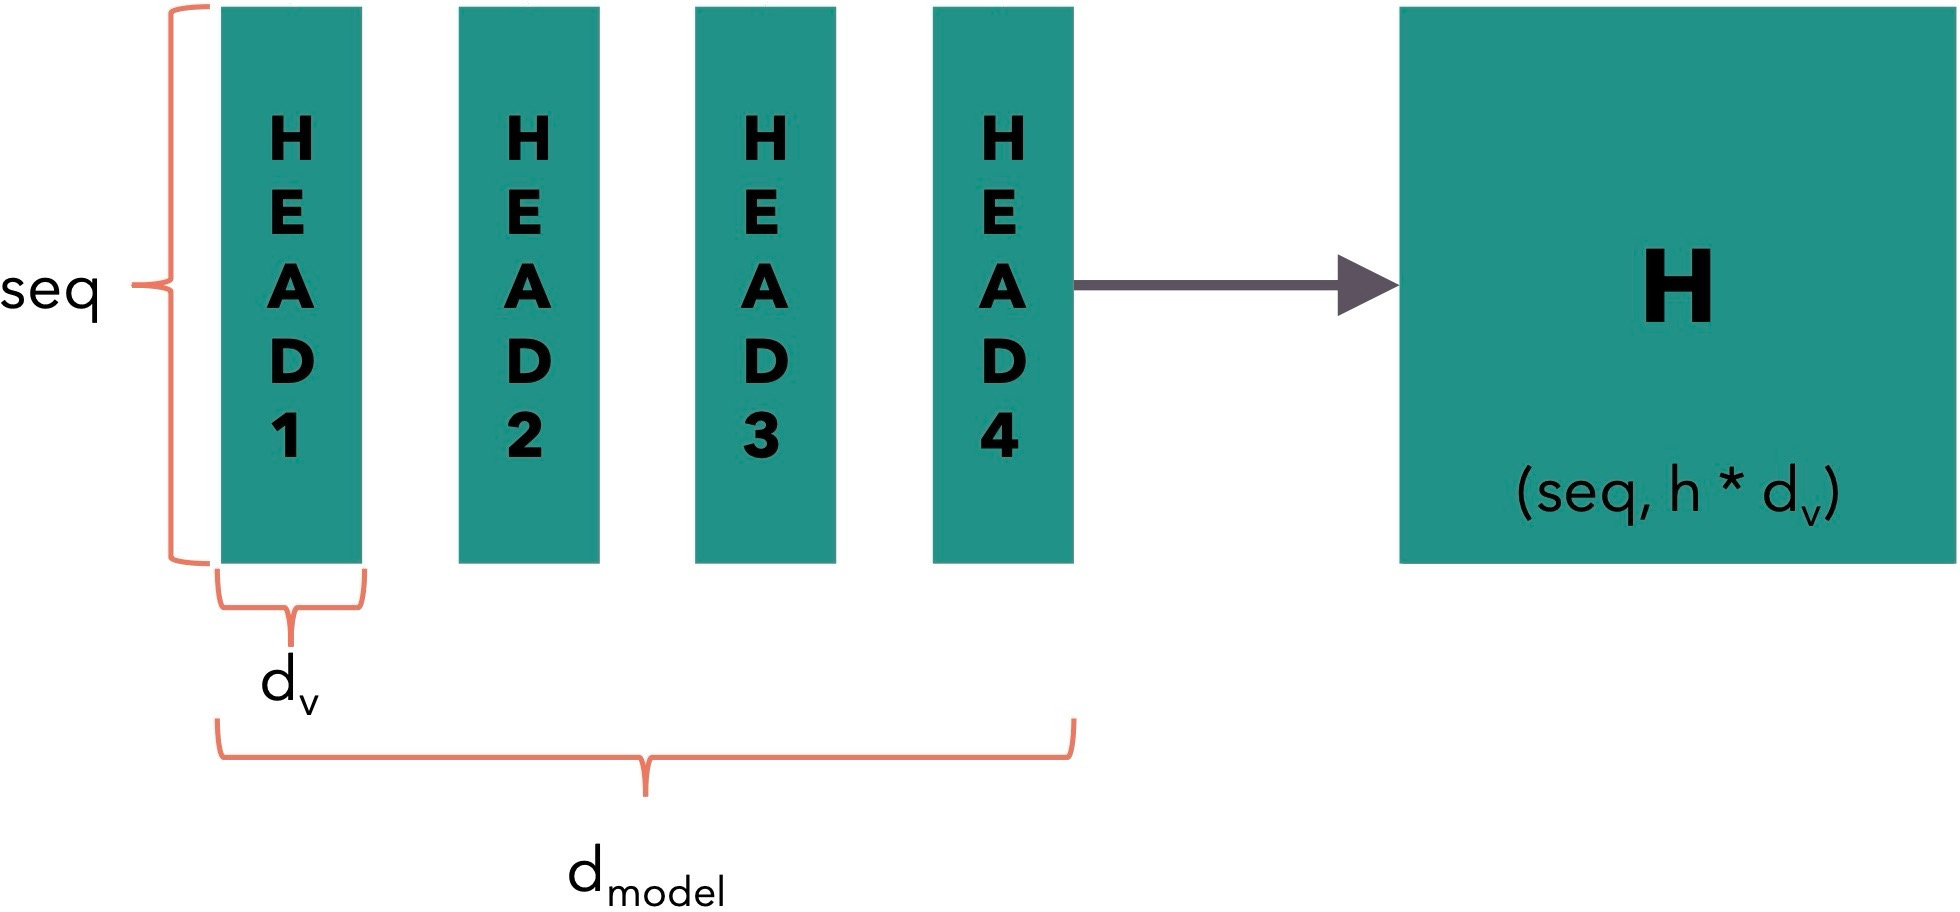
\includegraphics[width=0.55\linewidth]{img/mh-step-3.jpeg}
\caption{\textbf{(Alternative Approach, \textit{Step 3})} The head matrices obtained as a result of Self-Attention are concatenated along axis 1 \cite{git-hub}. The result is a matrix $H$ of dimension ${seq\times (h\cdot d_v)}$.}
\label{fig:mh_step3}
\end{figure}

\paragraph{Final Projection}
Finally, the concatenated output is projected through the final weight matrix $W^O \in \mathbb{R}^{(h\cdot d_v)\times d_{model}}$ \cite{arxiv-attention, stanford}:
$$
MultiHead(Q, K, V)=Concat(head_1, head_2, \dots, head_h)W^O \in \mathbb{R}^{seq\times d_{model}}
$$
Note how, in this case as well (analogously to Self-Attention), the output matrix has the same dimension $seq\times d_{model}$ as the input matrix $X$ \cite{arxiv-attention, git-hub}.

\begin{figure}[H]
\centering
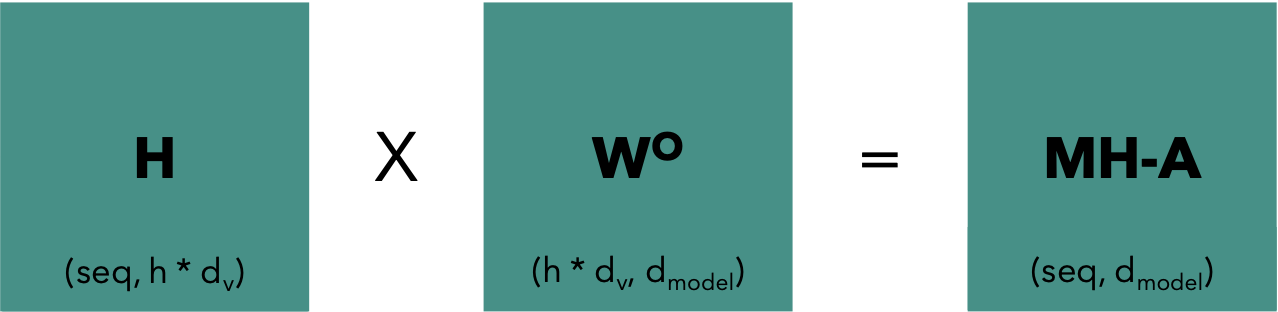
\includegraphics[width=0.65\linewidth]{img/mh-step-4.png}
\caption{\textbf{(Alternative Approach, \textit{Step 4})} The concatenated matrix $H$ is projected onto the output matrix $W^O \in \mathbb{R}^{(h \cdot d_v) \times d_{model}}$, producing the resulting matrix $MH\_A \in \mathbb{R}^{seq \times d_{model}}$ \cite{git-hub}. The matrix $MH\_A$ thus constitutes the result of Multi-Head Attention.}
\label{fig:mh_step}
\end{figure}



%\subsubsection{Layer Normalization e Residual Connections}
%\label{sub:layer_norm_residual_connection}
%\noindent
%Questi componenti sono essenziali per la stabilità numerica e la convergenza durante l'addestramento. Esistono due convenzioni principali: post-LN e pre-LN, con quest'ultima che ha dimostrato maggiore facilità di addestramento.

\subsection{Normalization and Residual Mechanisms}
As shown in Figure \ref{fig:transformer}, applied to each sub-layer of the Transformer (Multi-Head Attention and Feed-Forward Network) is a component called Add \& Norm \cite{arxiv-attention}, which combines two operations:
\begin{itemize}
\item \textbf{Add (Residual Connection):} Takes the output of a sub-layer (Multi-Head Attention or Feed Forward) and adds it to the original input of the same sub-layer \cite{arxiv-attention, arxiv-skipconnection-survey}.
\item \textbf{Norm (Layer Normalization):} Applies a normalization that standardizes the vector values for each token in the sequence \cite{arxiv-attention, stanford}.
\end{itemize}
This component plays a fundamental role in maintaining training stability and enabling the training of deep networks \cite{arxiv-attention, arxiv-skipconnection-survey}.

\subsubsection{Residual Connection (Add)}
A residual connection, or skip connection, is a direct path connecting the input of a sub-layer to its output, bypassing the sub-layer itself \cite{arxiv-attention, arxiv-skipconnection-survey}:
\begin{equation}
Output_{residual} = x + SubLayer(x)
\end{equation}

where:
\begin{itemize}
\item $x$ represents the input of the \textit{SubLayer}
\item $SubLayer(x)$ represents the output of the \textit{SubLayer}
\end{itemize}
The benefits provided by the application of this state are:
\begin{itemize}
\item \textbf{Mitigation of the Vanishing Gradient Problem:} The primary advantage of residual connections is that they allow the gradient to bypass the sub-layer during backpropagation \cite{arxiv-skipconnection-survey}. Formally, the gradient of the loss function $L$ with respect to the input $x$ is:
\begin{equation}
\frac{\partial L}{\partial x} = \frac{\partial L}{\partial Output_{residual}} \frac{\partial Output_{residual}}{\partial x}
\end{equation}

Calculating $\frac{\partial Output_{residual}}{\partial x}$ separately, we obtain:
$$
\frac{\partial Output_{residual}}{\partial x} = \frac{\partial \left(x + SubLayer(x)\right)}{\partial x} = \frac{\partial x}{\partial x} + \frac{\partial SubLayer(x)}{\partial x} = 1 + \frac{\partial SubLayer(x)}{\partial x}
$$
This yields:
$$
 \frac{\partial L}{\partial x} = \frac{\partial L}{\partial Output_{residual}} \left( 1 + \frac{\partial SubLayer(x)}{\partial x} \right)
$$

Note how the term $1$ guarantees the existence of a path with a non-zero gradient, regardless of how small $\frac{\partial SubLayer(x)}{\partial x}$ becomes \cite{arxiv-skipconnection-survey}. This characteristic prevents the vanishing gradient problem, where gradients become exponentially smaller across layers, making the training of deep networks impossible \cite{arxiv-attention, arxiv-skipconnection-survey}.

\item \textbf{Information Preservation:} The residual connection preserves the original information from the input, ensuring that crucial information is not lost within the sub-layer \cite{arxiv-skipconnection-survey}. The sub-layer only adds its contribution, but the original information is always present.

\item \textbf{Depth Stability:} It allows for the training of very deep Transformers without performance degradation at inference time \cite{arxiv-attention, arxiv-skipconnection-survey}. It has been demonstrated that adding more layers without residual connections often worsens performance; with residual connections, adding layers generally improves or maintains performance during inference.
\end{itemize}

\subsubsection{Layer Normalization (Norm)}
Layer Normalization is a technique that normalizes activation values along the feature (embedding) dimension rather than along the batch dimension (as performed in Batch Normalization) \cite{batch_norm}.

\begin{figure}[H]
\centering
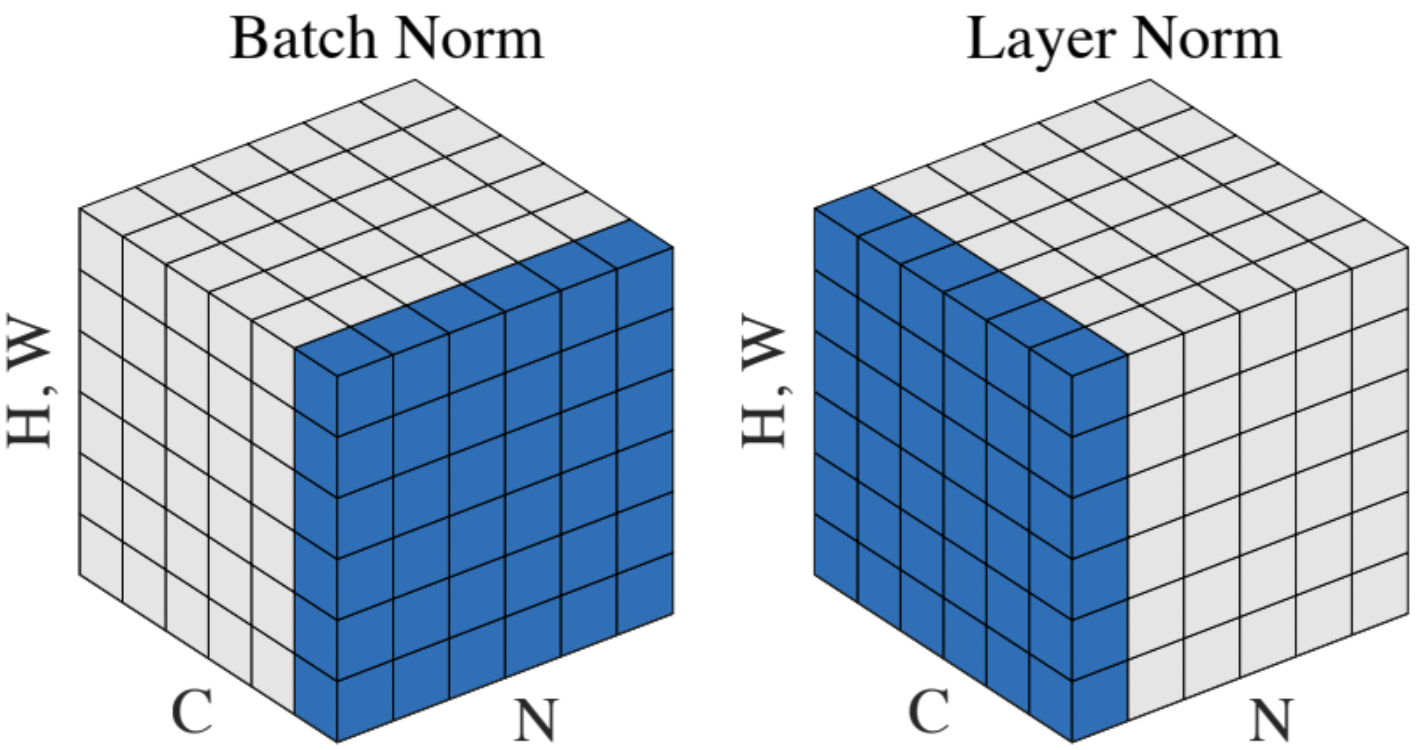
\includegraphics[width=0.5\linewidth]{img/batch_vs_norm.png}
\caption{Graphical representation of the difference between \textbf{Batch Normalization} (left) and \textbf{Layer Normalization} (right) via two 3D tensors with dimensions \textit{N} (batch), \textit{C} (channels/features), \textit{H} (height), and \textit{W} (width) \cite{batch_norm}. The blue region highlights the dimensions along which normalization statistics (mean and variance) are calculated. Note that in \textbf{Batch Norm}, this occurs vertically along \textit{N}, making it dependent on the batch size \cite{batch_norm}; in \textbf{Layer Norm}, it occurs horizontally along C, H, and W (thus independent of the batch) \cite{batch_norm}, which is ideal for variable sequences such as in Transformers.}
\label{fig:batch_vs_layer_norm}
\end{figure}

Formally, for each token $i$ in the sequence, given the activation vector $x_i\in \mathbb{R}^{d_{model}}$, Layer Normalization computes \cite{arxiv-attention, stanford}:
\begin{equation}
LayerNorm(x_i)= \gamma \odot \frac{x_i - \mu}{\sqrt{\sigma^2 + \epsilon}} + \beta
\end{equation}

where:
\begin{itemize}
\item $\mu = \frac{1}{d_{model}} \sum^{d_{model}}_{j=1}x_{ij}$ is the mean of the activations for token $i$ across all its components
\item $\sigma^2_i=\frac{1}{d_{model}}\sum^{d_{model}}_{j=1} (x_{ij}-\mu_i)^2 $ is the variance
\item $\epsilon$ is a very small constant ($\approx 10^{-6}$) added for numerical stability
\item $\gamma \in \mathbb{R}^{d_{model}}$ is the learned \textit{scaling vector}
\item $\beta \in \mathbb{R}^{d_{model}}$ is the learned \textit{shift vector}
\item $\odot$ represents the element-wise product
\end{itemize}
The benefits provided by Layer Normalization are:
\begin{itemize}
\item \textbf{Gradient Stability:} Layer normalization maintains the scale of activations within a reasonable range (typically mean 0 and variance 1 after normalization), helping to prevent gradients from becoming too large (\textit{exploding gradients}) or too small (\textit{vanishing gradients}) \cite{arxiv-attention, stanford}.

\item \textbf{Mitigation of Internal Covariate Shift:} During training, the distribution of activations in each layer changes continuously (\textit{internal covariate shift}). This slows down training and requires smaller learning rates. Layer normalization reduces this effect \cite{arxiv-attention, stanford}.

\item \textbf{Improved Gradient Flow in Attention:} Input normalization enables the attention mechanism to operate on values with predictable scales \cite{arxiv-attention}. Without normalization, the dot products used in attention calculation could become very large, leading to "explosive" softmax values (close to 0 or 1) and consequently causing gradients to be dangerously close to zero \cite{arxiv-attention, stanford, GeeksForGeeks}.
\end{itemize}

\subsubsection{Configurations: Post-LN vs Pre-LN}
There are two common configurations for the Add \& Norm component in the Transformer \cite{git-hub, stanford}:
\begin{itemize}
\item \textbf{Post-LN} (Post-Normalization)
\item \textbf{Pre-LN} (Pre-Normalization)
\end{itemize}
In the original paper \textit{"Attention Is All You Need"}, the \textbf{Post-LN} configuration is used \cite{arxiv-attention}:
\begin{equation}
Output = LayerNorm(X + SubLayer(X))
\end{equation}

where:
\begin{itemize}
\item $X \in \mathbb{R}^{seq \times d_{model}}$ represents the input matrix of the \textit{sublayer}
\end{itemize}
In this manner, the residual is added first, and the normalization is applied only subsequently \cite{arxiv-attention, git-hub}.
This approach can ensure more stable training in some cases. Generally, however, the Post-LN configuration requires a learning rate \textit{warmup} phase to manage high-magnitude gradients close to the output layer \cite{arxiv-attention, stanford}.

In the \textbf{Pre-LN} configuration, used in modern models like \textit{GPT} and newer \textit{BERT} variants, \footnote{It is worth noting that while the original implementation of BERT used a Post-LN configuration\cite{xiong2020ln}, subsequent analyses and modern variants (and virtually all recent Large Language Models) have adopted Pre-LN or alternative normalizations (like RMSNorm)\cite{liu2023b2t,xiong2020ln} to improve training stability at greater depths\cite{liu2023b2t}.} we have:
\begin{equation}
Output = X + SubLayer(LayerNorm(X))
\end{equation}

Essentially, the input is first normalized, then passed to the sub-layer, and only finally is the residual connection added \cite{git-hub}.
The Pre-LN approach guarantees:
\begin{itemize}
\item High training stability without requiring learning rate \textit{warmup} \cite{git-hub, stanford}
\item Better gradients through the residual layers \cite{arxiv-skipconnection-survey, attention-is-not}
\item Higher learning rates \cite{git-hub, stanford}
\end{itemize}


\subsection{Position-wise Feed-Forward Networks}
The feed-forward layer (FFN), also referred to as the position-wise feed-forward network, is a fundamental component of the Transformer architecture \cite{arxiv-attention, attention-is-not} that accompanies the multi-head attention mechanism \cite{arxiv-attention}. This layer consists of a fully connected neural network \cite{arxiv-attention, stanford} that applies the same non-linear transformations to each token in the sequence, independently \cite{arxiv-attention, stanford, GeeksForGeeks}. In this manner, non-linearity is introduced into the Transformer architecture, which, consequently, becomes capable of learning complex non-linear relationships \cite{stanford, attention-is-not}.

The feed-forward layer is composed of two \textbf{linear} layers separated by a \textbf{non-linear} activation function \cite{arxiv-attention}. The structure can be represented as:
\begin{equation}
FFN(x)=\phi(x_iW_1 + b_1)W_2+b_2
\end{equation}

where:
\begin{itemize}
\item $x_i \in \mathbb{R}^{d_{model}}$ represents a single token with $i=\{1,\dots, seq\}$
\item $W_1 \in \mathbb{R}^{d_{model}\times(4\cdot d_{model})}, W_2 \in \mathbb{R}^{(4 \cdot d_{model})\times d_{model}}$ represent the weight matrices
\item $b_1 \in \mathbb{R}^{4\cdot d_{model}}, b_2\in \mathbb{R}^{d_{model}}$ represent the bias vectors
\item $\phi$ represents the activation function (obviously non-linear)
\end{itemize}

In the original Transformer, the activation function $\phi$ is a simple $ReLU(x)$ \cite{arxiv-attention}, but in more modern implementations, it is often implemented as $GELU$ or $SwiGLU$ \cite{stanford, attention-is-not}. \footnote{Unlike ReLU, which outputs strictly zero for negative inputs (potentially causing the 'dying ReLU' problem), functions like GELU (Gaussian Error Linear Unit) are smooth and non-monotonic \cite{stanford}. This allows for better gradient flow and has been empirically shown to improve convergence in deep Transformer models (e.g., BERT, GPT-3) \cite{stanford, attention-is-not}.}
%\begin{center}
%\begin{tikzpicture}[
 % node distance=1cm and 1.5cm,
%layer/.style={rectangle, draw, minimum width=2.5cm, minimum height=1cm, align=center},
 % arrow/.style={-Straight Barb, thick}
%]

% Nodi del diagramma
%\node (input_arrow) {$x_i$}; % Punto di partenza per la freccia di input
%\node (linear1) [layer, below=of input_arrow] {Linear};
%\node (relu)[layer, below=of linear1] {ReLU};
%\node (linear2) [layer, below=of relu]{Linear};
%\node (output_arrow) [below=of linear2] {$FFN(x_i)$}; % Punto di arrivo

% Frecce che collegano i layer
%\draw[arrow] (input_arrow) -- (linear1);
%\draw[arrow] (linear1) -- (relu);
%\draw[arrow] (relu)-- (linear2);
%\draw[arrow] (linear2) -- (output_arrow);

%\end{tikzpicture}
%\end{center}


\begin{figure}[H]
\centering
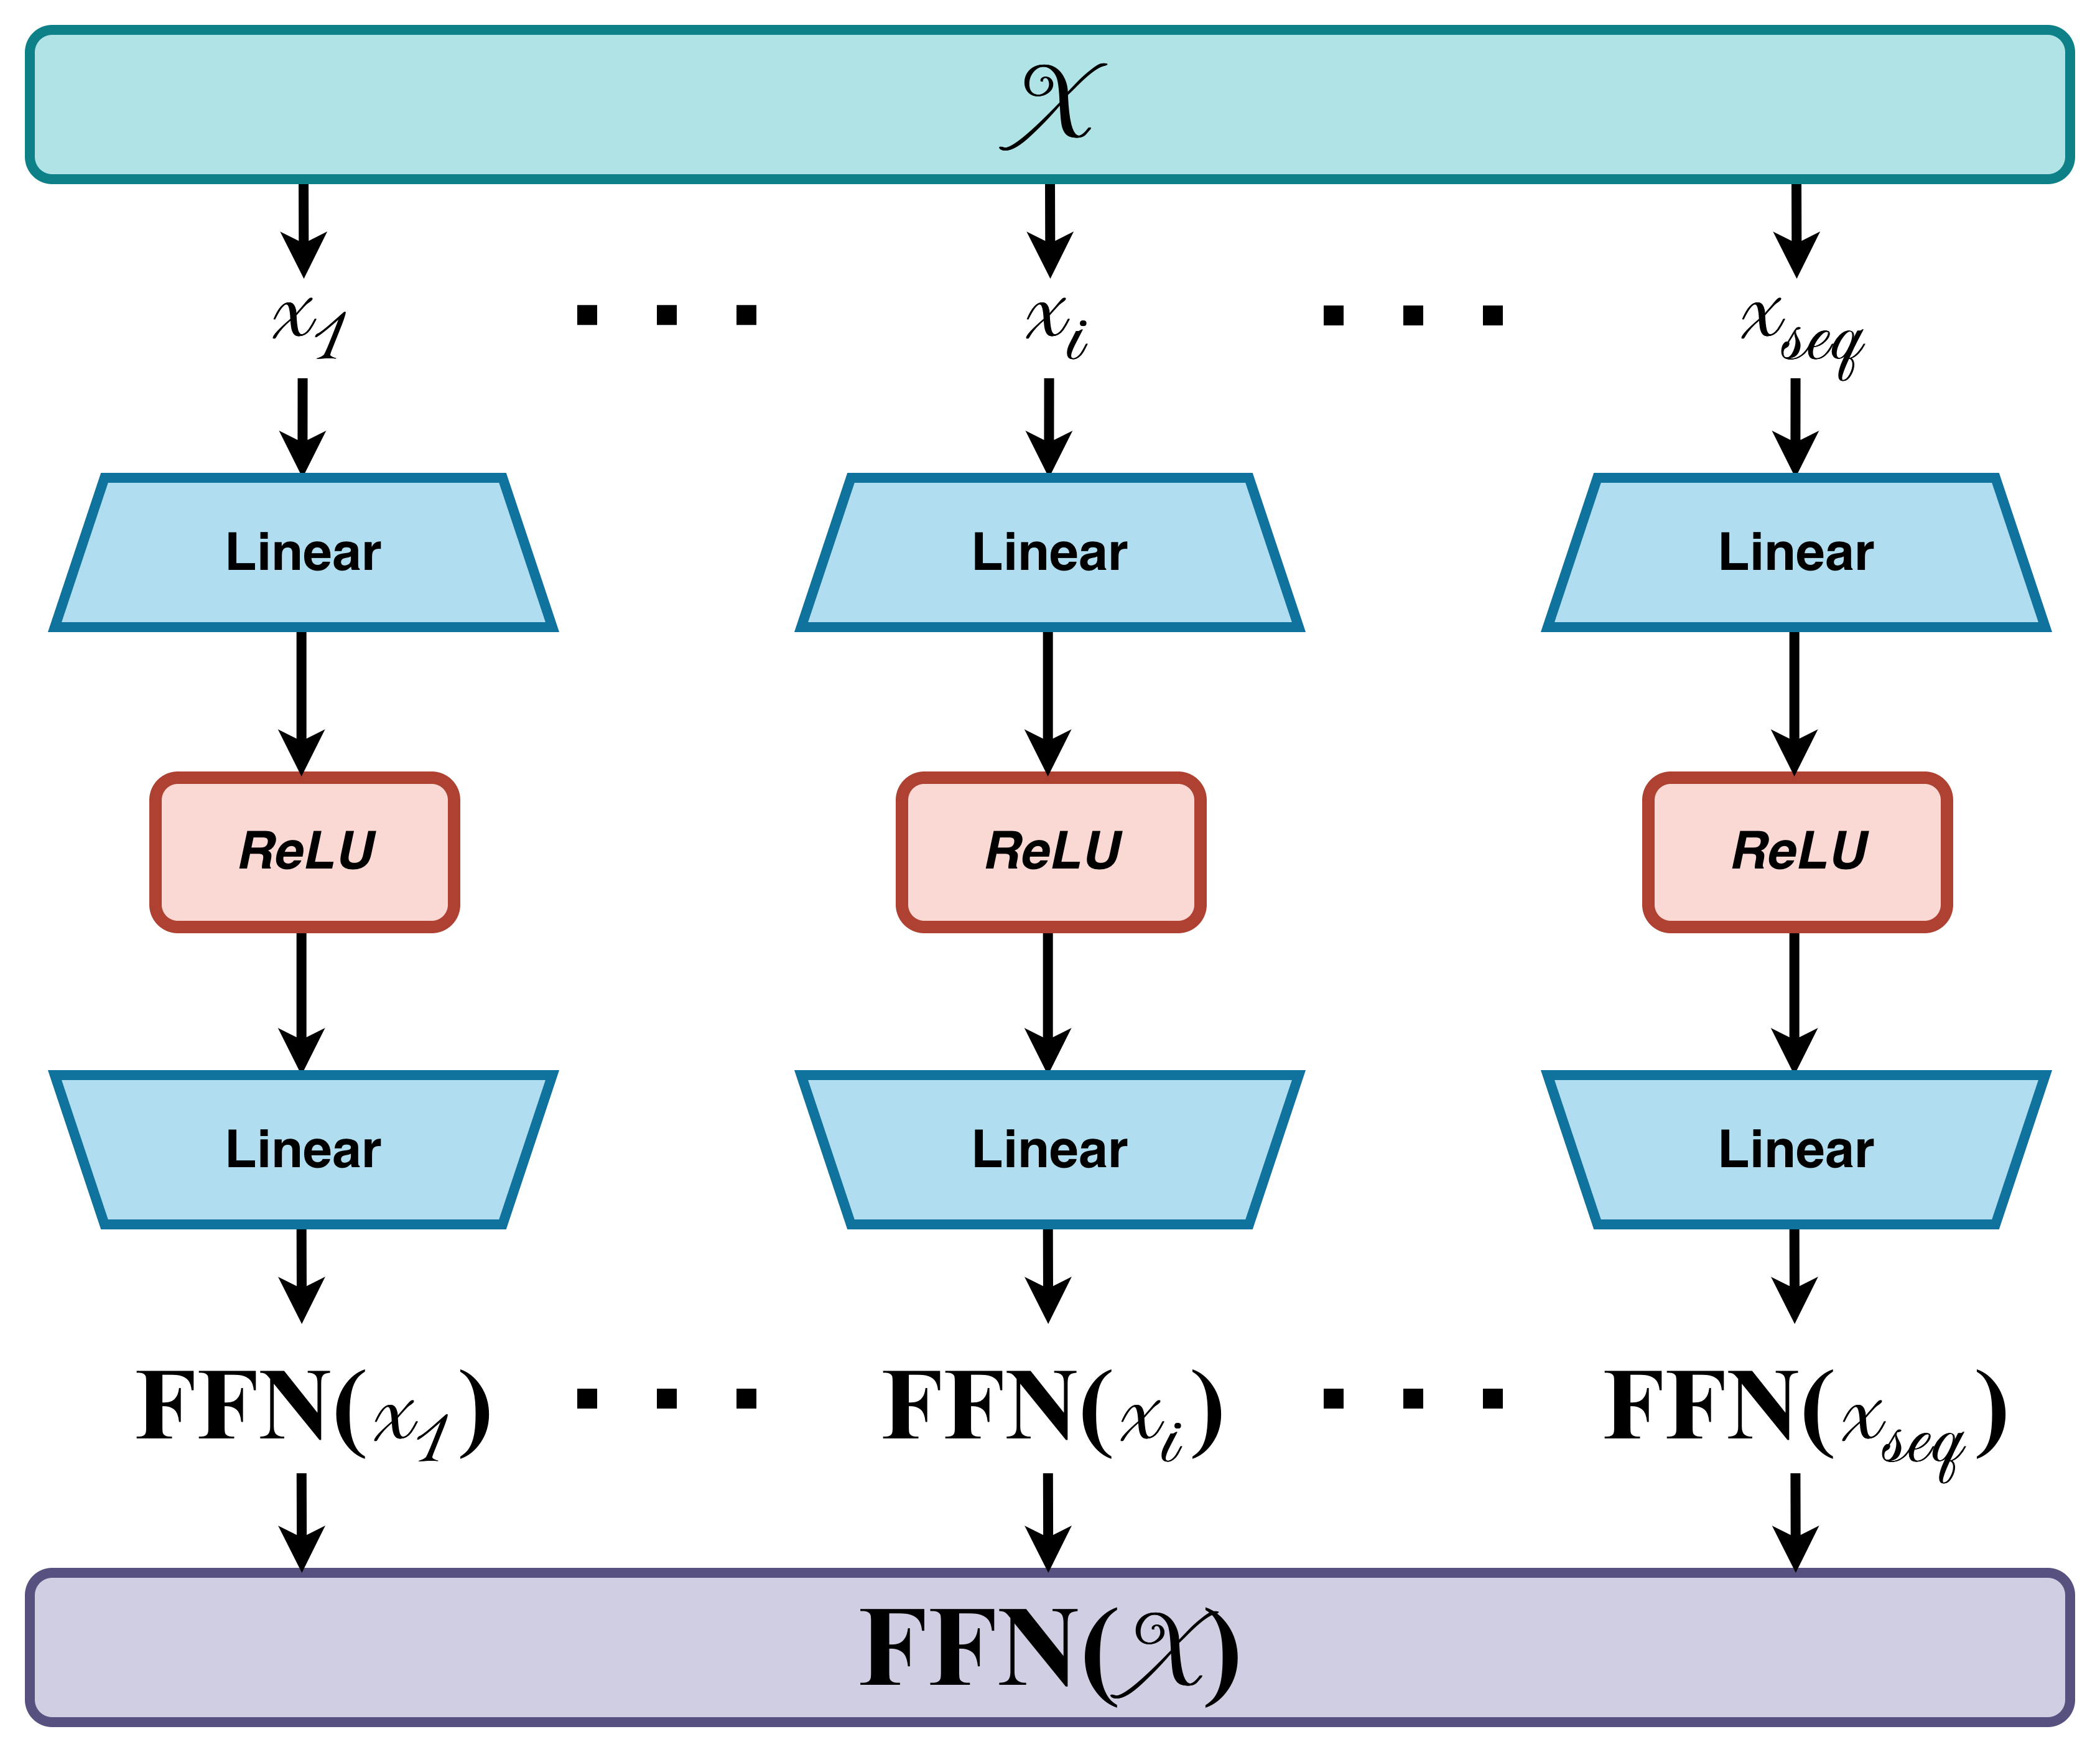
\includegraphics[width=0.5\linewidth]{img/ffn_3.png}
\caption{Schematic representation of the feed-forward network. The operations are shown in sequence: linear transformation (expanding the dimensionality), application of the ReLU activation function, and a second linear transformation (projecting back to the original dimensionality).}
\label{fig:ffn}
\end{figure}
The feed-forward layer thus complements the attention mechanism \cite{attention-is-not}; indeed, while attention mixes and weighs information originating from different tokens in the sequence (in a linear manner), the FFN applies further processing to each token individually, enabling the model to capture complex and non-linear patterns \cite{attention-is-not}.

\subsection{Encoder-Decoder: Integration of the Transformer Architecture}
Up to this point, the components of the Transformer architecture have been examined individually: tokenization, the self-attention mechanism, multi-head attention, residual connections, layer normalization, and the feed-forward network. Each of these elements plays a specific role in information processing. The aim of this section is to integrate all this knowledge to understand how the encoder and decoder work together, forming an architecture capable of transforming an input sequence into a plausible output sequence while maintaining semantic context and long-range relationships.

\subsubsection{Encoder}
The encoder consists of $N$ identical layers stacked sequentially (in the original paper, $N=6$ is used) \cite{arxiv-attention}.
Each encoder layer contains two sub-layers \cite{arxiv-attention, stanford}:
\begin{enumerate}
\item \textbf{Multi-Head Self-Attention:} Allows the tokens of the initial sequence to relate to one another \cite{arxiv-attention, GeeksForGeeks}.
\item \textbf{Position-wise Feed-Forward Network:} Applies non-linear transformations to each token independently, enabling the model to learn complex non-linear relationships \cite{arxiv-attention, attention-is-not}.
\end{enumerate}
Each of these two sub-layers is then followed (or preceded) by an Add \& Norm component, which applies a skip connection and layer normalization \cite{arxiv-attention, git-hub}.

The output of the final encoder layer $N$ consists of an output matrix $E^{(N)} \in \mathbb{R}^{seq \times d_{model}}$, representing a contextualized embedding of each token in the input sequence, enriched with information coming from all other tokens in the sequence via the self-attention mechanisms \cite{arxiv-attention, stanford, hashnode}.
\begin{figure}[H]
\centering
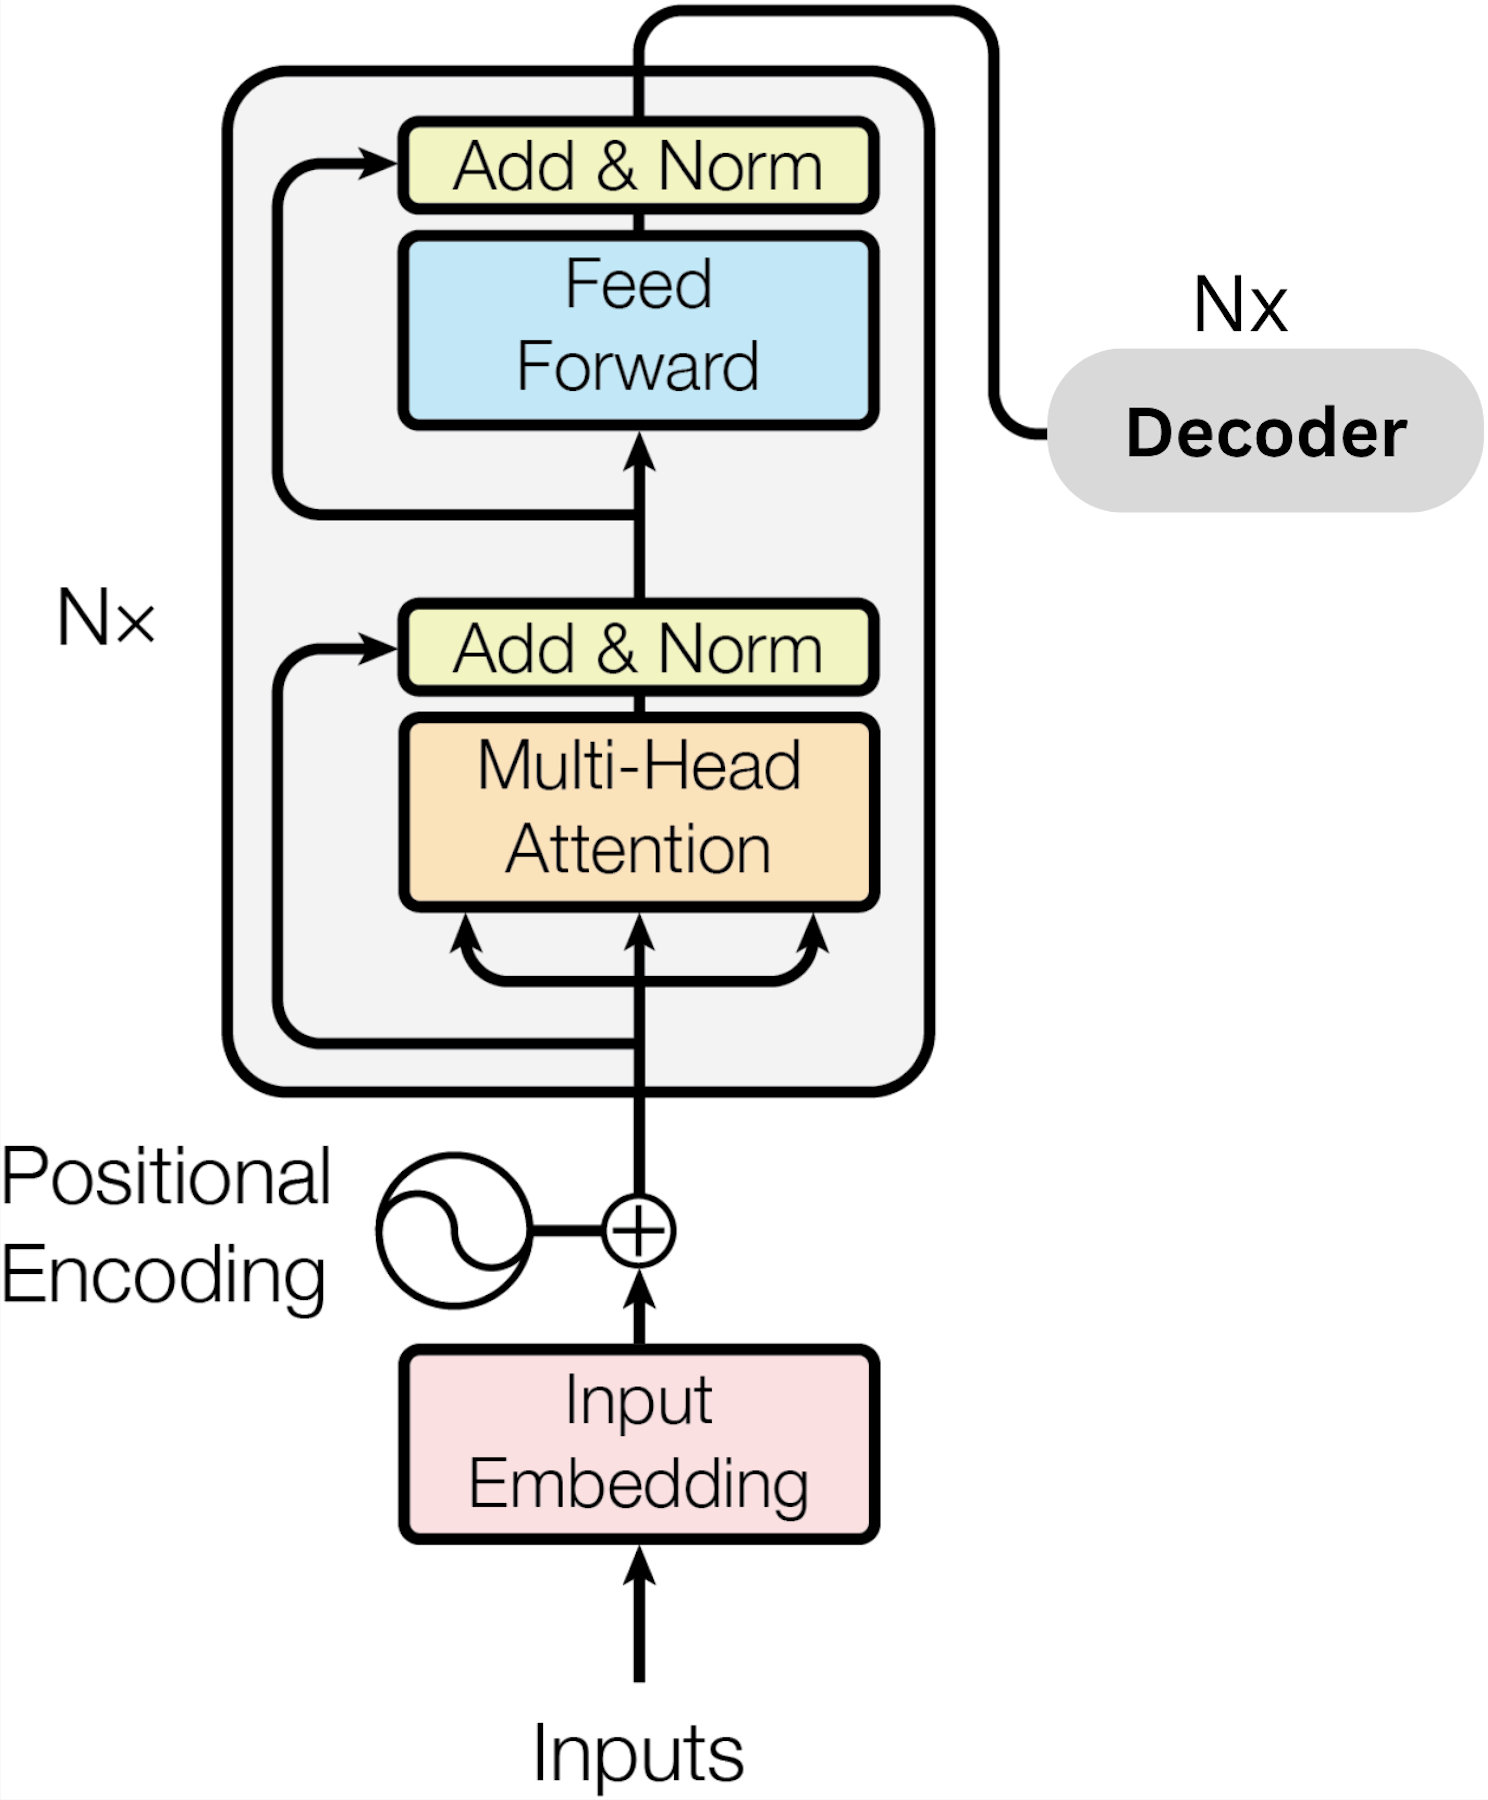
\includegraphics[width=0.5\linewidth]{img/encoder-schema_3.png}
\caption{Schematic representation of the flow followed by the input sequence within the $N$ encoder layers. The output matrix $E^{(N)} \in \mathbb{R}^{seq \times d_{model}}$ is sent to the Decoder \cite{arxiv-attention}.}
\label{fig:encoder_schema}
\end{figure}
The properties of the encoder include:
\begin{itemize}
\item \textbf{Breaking of Permutation Equivariance:} Due to positional encoding, the encoder does not possess the property of permutation equivariance; the sequence order is thus explicitly represented \cite{arxiv-attention, Muhammad_Faizan}.

\item \textbf{Full Context Access:} Each token has access to all other tokens in the sequence, allowing for the capture of global dependencies \cite{arxiv-attention, stanford, GeeksForGeeks}.

\item \textbf{Total Parallelization:} All tokens can be processed simultaneously, making the encoder computationally efficient on \textit{GPUs} \cite{arxiv-attention}.
\end{itemize}

\subsubsection{Decoder}
The decoder features a structure similar to that of the encoder; however, it is divided into three sub-layers \cite{arxiv-attention, stanford}:
\begin{enumerate}
\item \textbf{Masked Multi-Head Self-Attention:} Self-attention on a masked version of the output sequence \cite{arxiv-attention, GeeksForGeeks}.
\item \textbf{Multi-Head Cross-Attention:} Attention between the decoder tokens and the encoder representation \cite{arxiv-attention, hashnode}.
\item \textbf{Position-wise Feed-Forward Network:} Analogous to the encoder sub-layer \cite{arxiv-attention, attention-is-not}.
\end{enumerate}
In this case as well, each sub-layer is followed (or preceded) by an Add \& Norm component that applies a skip connection and layer normalization \cite{arxiv-attention, git-hub}.
The decoder, analogous to the encoder, consists of $m=\{1, 2, \dots, N\}$ layers \cite{arxiv-attention}.
\begin{figure}[H]
\centering
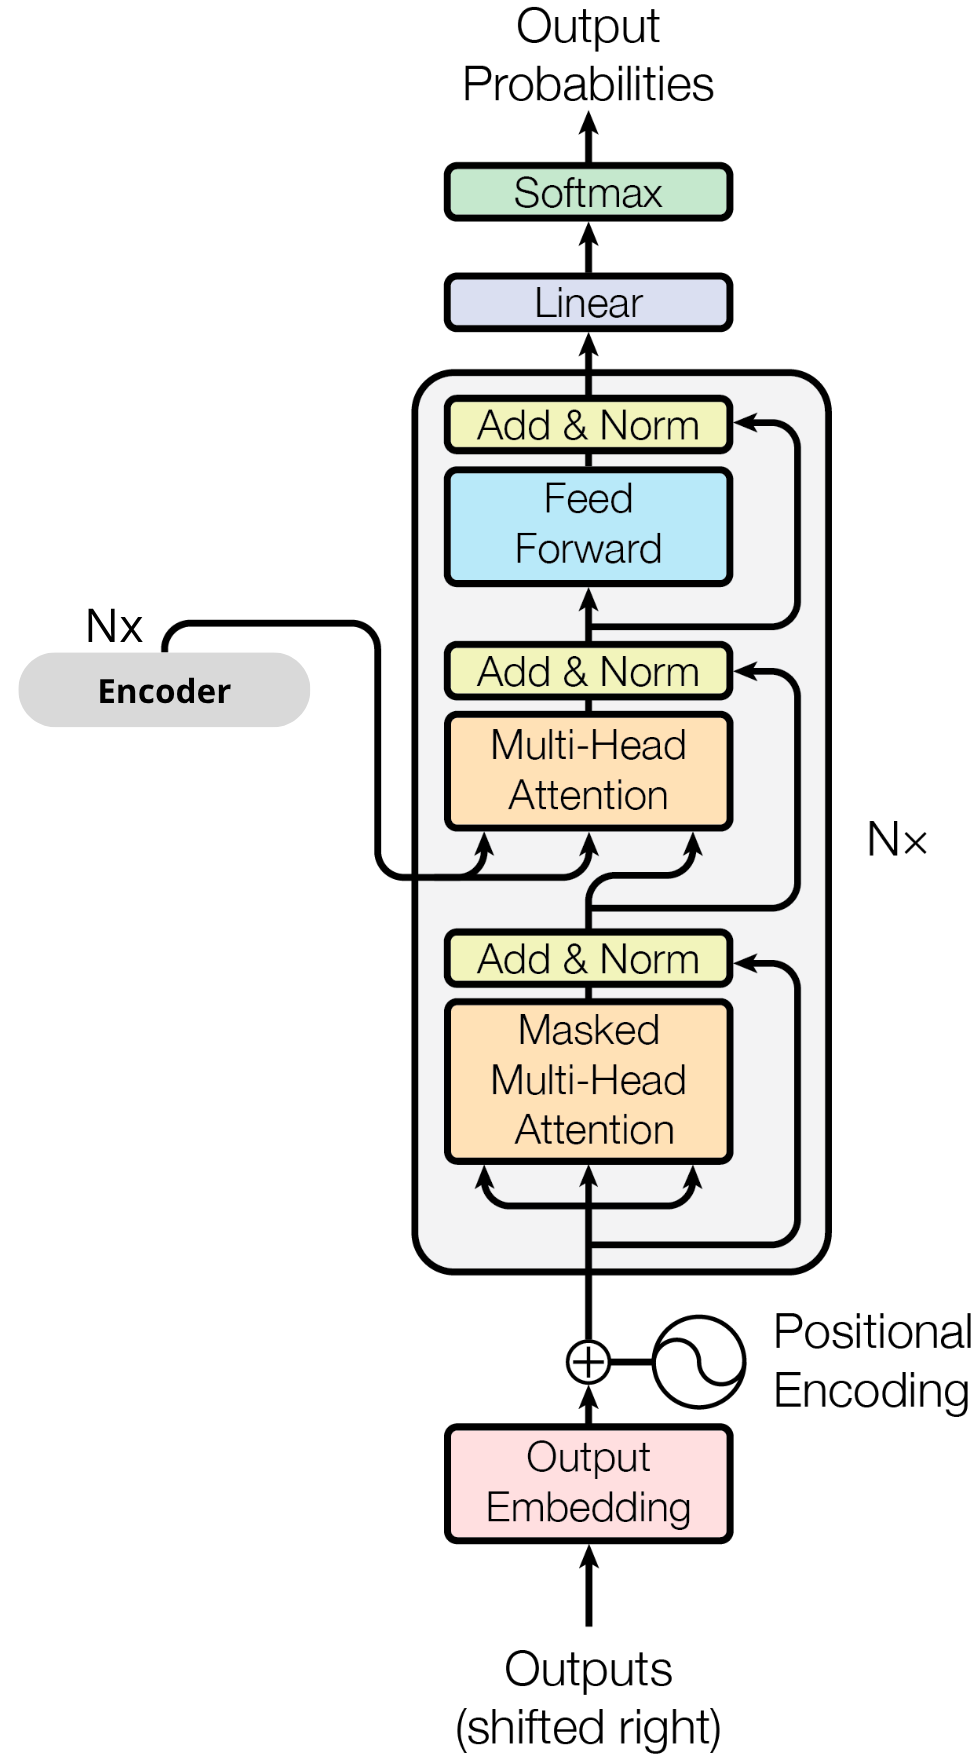
\includegraphics[width=0.5\linewidth]{img/decoder-schema_2.png}
\caption{Schematic representation of the flow followed by the input sequence within the $N$ decoder layers \cite{arxiv-attention}.}
\label{fig:schema}
\end{figure}
The various internal phases of the decoder are described below:

\paragraph{Masked Self-Attention}
The crucial difference compared to the encoder lies in the decoder's self-attention mechanism \cite{arxiv-attention}. During training, the model must generate output individually for each token $x_i$, without access to future tokens ($x_{i+1}, x_{i+2}, \dots$) \cite{arxiv-attention, stanford}. For this reason, a "mask" is applied to the attention matrix \cite{arxiv-attention, GeeksForGeeks}.



During the calculation of the $Attention$ matrix, before applying the $softmax$, a very large negative value (typically $-\infty$) is added to future positions \cite{arxiv-attention, hashnode}.\footnote{This training strategy, where the model is fed the actual ground-truth tokens from the previous steps rather than its own generated predictions, is formally known as \textit{Teacher Forcing} \cite{stanford}. It enables parallelization during training, unlike the sequential generation required during inference.} A mask matrix $M\in \mathbb{R}^{seq\times seq}$ is therefore added:
\begin{equation}
Attention(Q_i,K_i,V_i) = softmax\left( \frac{QK^T}{\sqrt{d_k}} + M\right)V
\end{equation}

The mask matrix is defined for each token $x_i$ as:
$$
M=
\begin{cases}
\quad 0 \quad \quad \textit{ if}\quad i \ge j \\
-\infty \quad \quad \textit{if} \quad i < j
\end{cases}
$$
where:
\begin{itemize}
\item $i$ indicates the rows of $M$
\item $j$ indicates the columns of $M$
\end{itemize}
The mask matrix will therefore be of the form:
%%%%%% MATRICE NELL'ALTRA FORMA, SCEGLI QUALE USARE.
%$$
 % M = 
%\begin{bmatrix}
%0 & -\infty & -\infty & \cdots & -\infty \\
%0 & 0 & -\infty & \cdots & -\infty \\
%0 & 0 & 0 & \cdots & -\infty \\
%\vdots & \vdots & \vdots & \ddots & \vdots \\
%0 & 0 & 0 & \cdots & 0
%\end{bmatrix}_{seq \times seq}
%$$
$$
M = 
\begin{pmatrix}
0 & -\infty & -\infty & -\infty & \cdots & -\infty \\
0 & 0 & -\infty & -\infty & \cdots & -\infty \\
0 & 0 & 0 & -\infty & \cdots & -\infty \\
\vdots & \vdots & \vdots & \vdots & \ddots & \vdots \\
\vdots & \vdots & \vdots & \vdots & \ddots & \vdots \\
0 & 0 & 0 & \cdots & \cdots & 0
\end{pmatrix}_{seq \times seq}
$$
This configuration ensures that the calculation of the $softmax$, in positions $j > i$, returns a probability value of $0$ for future tokens.
\begin{figure}[H]
\centering
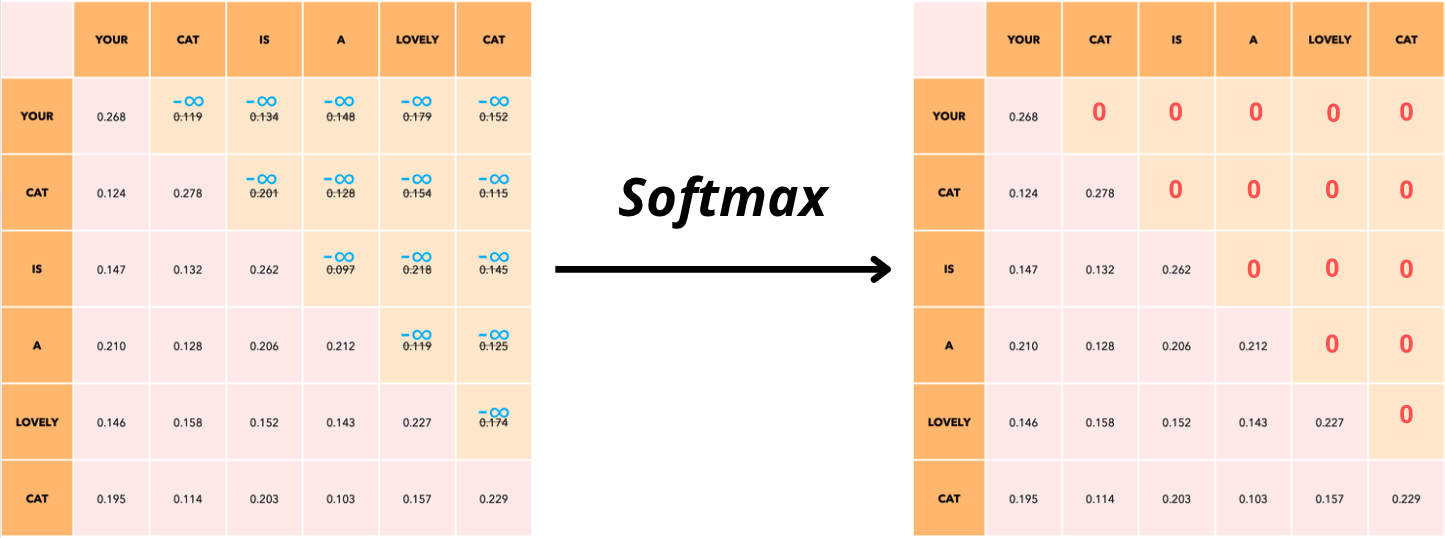
\includegraphics[width=1\linewidth]{img/masked_process.png}
\caption{Example of applying the mask matrix $M\in \mathbb{R}^{seq\times seq}$ to the matrix $\frac{QK^T}{\sqrt{d_k}}$ (left) and the subsequent application of the $softmax$ function \cite{git-hub}. The resulting $AttentionWeights$ matrix (right) presents a score of $0$ on every $token_j$ where $j>i$.}
\label{fig:masked_process}
\end{figure}

\paragraph{Cross-Attention} The second sub-layer of the decoder introduces the cross-attention mechanism \cite{arxiv-attention}. Unlike self-attention, in this case:
\begin{itemize}
\item The Query matrix $Q \in \mathbb{R}^{seq_{out} \times d_k}$ originates from the decoder output sequence of the previous layer \cite{arxiv-attention, hashnode}.
\item The Key matrix $K\in \mathbb{R}^{seq \times d_k}$ and the Value matrix $V \in \mathbb{R}^{seq \times d_v}$ originate from the encoder representation \cite{arxiv-attention, stanford}.
\end{itemize}
Formally:
$$
CrossAttention^{(m)} = MultiHeadAttention(Q_{decoder^{(m-1)}}, K_{encoder}, V_{encoder})
$$
where:
\begin{itemize}
\item $Q_{decoder^{(m-1)}} \in \mathbb{R}^{seq_{out}^{(m-1)} \times d_k}$ represents the query from the previous decoder layer $m-1$.
\end{itemize}
The Cross-Attention mechanism thus allows the model, using the Query matrix, to search for and extract information from the Key and Value matrices \cite{hashnode, stanford}.

\paragraph{Generation of the Final Output Matrix}
According to the architecture described in \textit{"Attention Is All You Need"} \cite{arxiv-attention}, following each Cross-Attention phase, the resulting matrix $CrossAttention^{(m)}$ passes through:
\begin{enumerate}
\item \textbf{Residual Connection + Layer Normalization} \cite{arxiv-attention, arxiv-skipconnection-survey}
\item \textbf{Position-wise Feed-Forward Network} \cite{arxiv-attention, attention-is-not}
\item \textbf{Residual Connection + Layer Normalization} \cite{arxiv-attention, git-hub}
\end{enumerate}
The output of the decoder after $N$ layers is a representation $D^{(N)}\in \mathbb{R}^{seq_{out} \times d_{model}}$ \cite{arxiv-attention}, where each row represents an output token contextualized with respect to both the other output tokens and the entire input sequence \cite{stanford, hashnode}.

\subsubsection{Output Projection and Probability Distribution}
After passing through all $N$ encoder and decoder layers, the final sequence representation $D^{(N)}$ must be transformed into a probability distribution over the vocabulary $V$ \cite{arxiv-attention, stanford}.

The probability distribution over the vocabulary is produced in two phases \cite{arxiv-attention}:



\paragraph{Linear Layer} The representation matrix $D^{(N)}\in \mathbb{R}^{seq_{out} \times d_{model}}$ is projected onto a space with a dimension equal to the vocabulary size $|V|$ \cite{arxiv-attention, git-hub}. This operation produces the logits matrix $L \in \mathbb{R}^{seq_{out} \times |V|}$:
\begin{equation}
L = D^{(N)} W_{output} + b_{output}
\end{equation}

where:
\begin{itemize}
\item $W_{output} \in \mathbb{R}^{d_{model} \times |V|}$ represents the final output weight matrix
\item $b_{output}$ represents the final output bias vector
\end{itemize}

\paragraph{Softmax} The logits, represented by matrix $L$, are finally normalized via the softmax function to obtain the probability matrix $P \in \mathbb{R}^{seq_{out}\times |V|}$ for each output token \cite{arxiv-attention, stanford}. Each row $i$ of matrix $P$ represents a probability distribution over the vocabulary for the token at the $i$-th position of the output sequence \cite{stanford, GeeksForGeeks}.

Formally:
\begin{equation}
P_i = softmax(L_i) \quad \forall i \in \{1,2,\dots,seq_{out}\}
\end{equation}

where:
\begin{itemize}
\item $L_i \in \mathbb{R}^{|V|}$ represents the $i$-th row of $L$
\item $P_{i} \in \mathbb{R}^{|V|}$ represents the $i$-th row of $P$
\end{itemize}
Each element $P_{i,j}$ thus represents the probability predicted by the model that the token at position $i$ of the output sequence corresponds to the $j$-th token of the vocabulary \cite{arxiv-attention, hashnode}.

%%%%%%%%%%%%%%%%%%%%%%%%%%%%%%%%%%%%%%%%%%%%%%
% Capitolo 2 %
%%%%%%%%%%%%%%%%%%%%%%%%%%%%%%%%%%%%%%%%%%%%%%

%%%%%%%%%%%%%%%%%%%%%%%%%%%%%%%%%%%%%%%%%%%%%%
% CAPITOLO 2                                 %
%%%%%%%%%%%%%%%%%%%%%%%%%%%%%%%%%%%%%%%%%%%%%%
\include{chapters/related_work.tex}

%%%%%%%%%%%%%%%%%%%%%%%%%%%%%%%%%%%%%%%%%%%%%%
% CAPITOLO 3                                 %
%%%%%%%%%%%%%%%%%%%%%%%%%%%%%%%%%%%%%%%%%%%%%%
\chapter{Proposed Methodology and Mathematical Framework}
\label{chap:3}


\newpage

\begin{figure}[H]
    \centering
    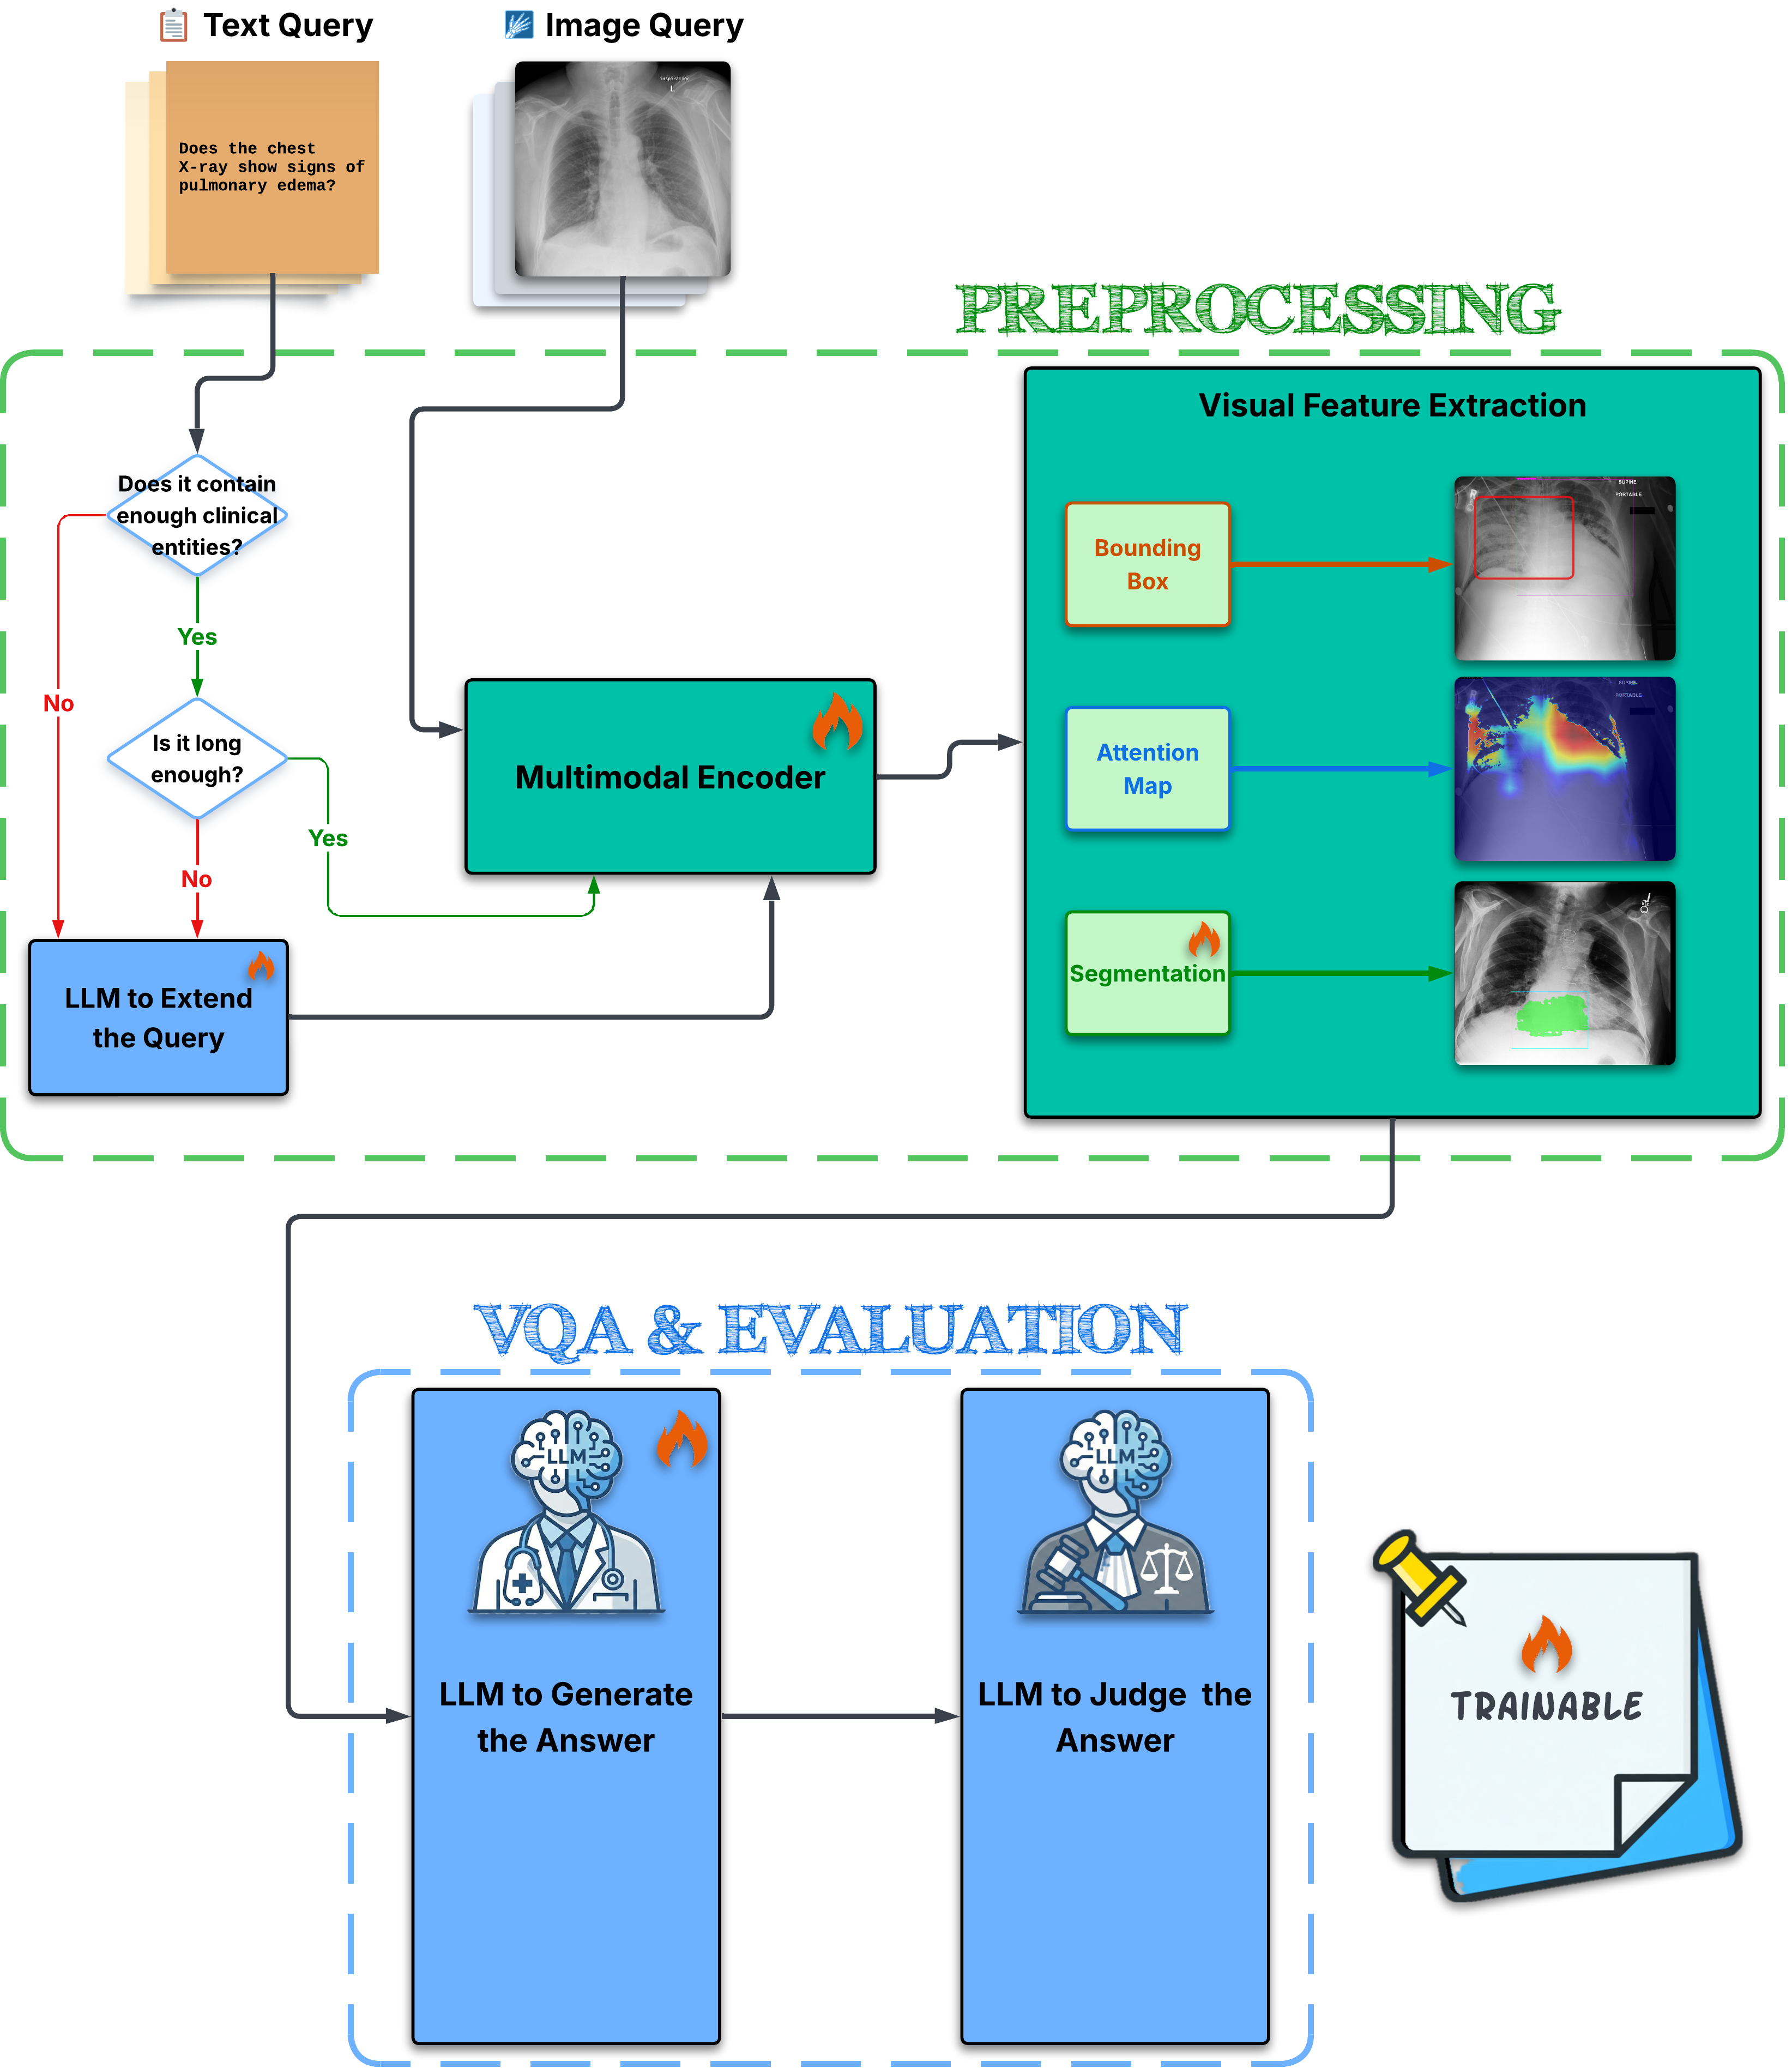
\includegraphics[width=1\linewidth]{real_pipeline.png}
    \caption{Enter Caption}
    \label{fig:placeholder}
\end{figure}

\section{Architectural Overview of the Pipeline}
\label{sec:3_1}
\subsection{Core Concept: Visual Grounding for Medical VQA}
\label{sec:3_1_1}

The central thesis underpinning the proposed system is that a Medical Visual Question Answering (VQA) model achieves superior diagnostic accuracy when it is not required to attend to an entire radiographic image indiscriminately, but is instead presented with a \textit{visually prompted} image in which the clinically relevant Regions of Interest (RoIs) have been explicitly highlighted. This paradigm, referred to throughout this work as \textbf{Visual Grounding}, transforms the VQA task from an unconstrained whole-image reasoning problem into a focused, region-aware inference problem.

Formally, let the raw input to the system be defined as a tuple $(\mathbf{I}, q)$, where $\mathbf{I} \in \mathbb{R}^{H \times W \times C}$ denotes a medical image (e.g., a chest X-ray) of height $H$, width $W$, and $C$ colour channels, and $q \in \mathcal{V}^*$ denotes a free-text clinical question drawn from the Kleene closure over a medical vocabulary $\mathcal{V}$. The objective of Visual Grounding is to construct an augmented image $\mathbf{I}' \in \mathbb{R}^{H \times W \times C}$ that encodes spatial emphasis on diagnostically salient regions, conditioned on the semantic content of $q$. The downstream VQA model $\mathcal{M}_{\text{VQA}}$ then operates on the pair $(\mathbf{I}', q)$ rather than $(\mathbf{I}, q)$, yielding a predicted answer:

\[
a^{*} = \mathcal{M}_{\text{VQA}}(\mathbf{I}', q)
\]

where:
\begin{itemize}
\item $a^{*}$ represents the predicted answer generated by the VQA model
\item $\mathcal{M}_{\text{VQA}}$ represents the downstream Vision-Language Model used for diagnostic answer generation
\item $\mathbf{I}' \in \mathbb{R}^{H \times W \times C}$ represents the visually prompted image encoding spatial emphasis on diagnostically salient regions
\item $q \in \mathcal{V}^*$ represents the free-text clinical question
\end{itemize}

The hypothesis is that the conditional mutual information between the answer $a^{*}$ and the ground-truth answer $a_{\text{gt}}$ is maximised when the visual input carries explicit spatial priors aligned with the clinical query—i.e., $I\left(a^{*}; a_{\text{gt}} \mid \mathbf{I}', q\right) \geq I\left(a^{*}; a_{\text{gt}} \mid I, q\right)$.

This design philosophy departs from end-to-end VQA architectures that implicitly learn visual attention. Instead, it externalises the grounding step as an explicit, interpretable preprocessing pipeline, thereby enabling clinical transparency, modular substitution of components, and fine-grained control over the spatial prompting strategy.

\subsection{End-to-End Data Flow}
\label{sec:3_1_2}
The pipeline implements a strictly sequential transformation chain comprising four macro-stages, each of which consumes the output of its predecessor. The complete data flow is formalised as:

\[
(\mathbf{I}, q) \xrightarrow{\;\mathcal{S}_1\;} q' \xrightarrow{\;\mathcal{S}_2\;} \mathbf{A} \xrightarrow{\;\mathcal{S}_3\;} \mathbf{I}' \xrightarrow{\;\mathcal{S}_4\;} a^{*}
\]

where the four stages are defined as follows:

\begin{itemize}
    \item \textbf{Stage $\mathcal{S}_1$ --- Clinical NLP Analysis (Query Routing).} The raw question $q$ is analysed by a biomedical Named Entity Recognition (NER) module $\mathcal{N}$ to assess its clinical informativeness. If the question is deemed insufficiently detailed according to a formally defined criterion (cf. \ref{sec:3_2}), it is expanded into an enriched clinical prompt $q'$ via a generative language model $\mathcal{G}$. If the question already satisfies the quality criterion, it is passed through unchanged, i.e., $q' = q$. This stage ensures that the downstream vision model receives a textual query of sufficient clinical specificity to drive meaningful spatial attention.

    \item \textbf{Stage $\mathcal{S}_2$ --- Visual Localisation via Cross-Modal Attention.} The enriched query $q'$ and the original image $\mathbf{I}$ are jointly encoded by a contrastive vision-language model $f_{\text{VL}}$---a dual-encoder architecture comprising a Vision Transformer (ViT) backbone and a domain-specific biomedical text encoder, pre-trained on large-scale biomedical image-text corpora---and a class activation mapping algorithm (gScoreCAM) is applied to produce a spatial attention map $\mathbf{A} \in \mathbb{R}^{H \times W}$, where each element $\mathbf{A}_{i,j} \in [0, 1]$ quantifies the relevance of pixel $(i, j)$ to the clinical query $q'$. This attention map constitutes the core localisation signal from which all subsequent visual prompts are derived.

    \item \textbf{Stage $\mathcal{S}_3$ --- Visual Prompting.} The attention map $\mathbf{A}$ is transformed into a concrete visual overlay on the original image $\mathbf{I}$. This stage admits multiple parallel pathways (detailed in Section \ref{sec:3_1_3}), each of which produces a differently prompted image $\mathbf{I}'$. The pathways share the same upstream attention signal but differ in their prompting semantics---ranging from geometric bounding boxes to dense pixel-level segmentation masks.

    \item \textbf{Stage $\mathcal{S}_4$ --- VQA Inference.} The visually prompted image $\mathbf{I}'$ is paired with the clinical question $q$ (or its expanded variant $q'$) and fed to a Vision-Language Model (VLM) for answer generation. A separate evaluation module employing an LLM-as-a-Judge paradigm scores the generated answer against the gold-standard reference.
\end{itemize}

The entire pipeline can thus be expressed as a composite function:

\[
\mathcal{F} = \mathcal{S}_4 \circ \mathcal{S}_3 \circ \mathcal{S}_2 \circ \mathcal{S}_1
\]

where each $\mathcal{S}_i$ is a deterministic, self-contained transformation with well-defined input and output types. This compositional structure guarantees that any individual stage can be replaced, ablated, or extended without affecting the contract between adjacent stages. %—a property that is exploited extensively in the experimental evaluation (Chapter 4).

\subsection{Modularity: Multiple Visual Prompting Pathways}
\label{sec:3_1_3}
A distinctive architectural decision in the proposed system is the provision of three distinct \textbf{Visual Prompting Pathways}, all of which branch from the same shared attention signal $\mathbf{A}$ produced by Stage $\mathcal{S}_2$. Each pathway implements a different strategy for converting the continuous-valued attention map into a discrete or semi-discrete visual prompt overlaid on the original image. This multi-pathway design serves a dual purpose: it enables systematic ablation studies comparing prompting strategies, and it accommodates the heterogeneous requirements of different downstream VLMs (some of which respond more effectively to bounding boxes than to heatmaps, and vice versa).

The three pathways are defined as follows:

\begin{itemize}

    \item \textbf{Pathway $\mathcal{P}_{\text{bbox}}$ --- Bounding Box Prompting.} The attention map $\mathbf{A}$ is binarised via a threshold $\tau$ (optionally refined through Dense CRF post-processing), and contour extraction is performed on the resulting binary mask. Each connected component yields a bounding box $\mathbf{b}_k = (x_k^{\min}, y_k^{\min}, x_k^{\max}, y_k^{\max})$, which is rendered as a coloured rectangle on the image. An adaptive padding mechanism adjusts the box margins as a function of the relative box area, preventing both excessive cropping of small findings and unnecessary expansion of large ones. The prompted image is:

    \[
    \mathbf{I}'_{\text{bbox}} = \text{DrawBox}(\mathbf{I}, \{\mathbf{b}_k\}_{k=1}^{K})
    \]

    where:
    \begin{itemize}
    \item $\mathbf{I}'_{\text{bbox}}$ represents the visually prompted image with bounding box overlays
    \item $\text{DrawBox}$ represents the rendering function that overlays coloured rectangles on the original image
    \item $\mathbf{I}$ represents the original medical image
    \item $\{\mathbf{b}_k\}_{k=1}^{K}$ represents the set of $K$ extracted bounding boxes, where each $\mathbf{b}_k = (x_k^{\min}, y_k^{\min}, x_k^{\max}, y_k^{\max})$
    \end{itemize}

    \item \textbf{Pathway $\mathcal{P}_{\text{heat}}$ --- Heatmap Overlay Prompting.} The raw attention map $\mathbf{A}$ is normalised to $[0, 1]$, mapped through a perceptual colourmap $\phi : [0,1] \to \mathbb{R}^3$ (e.g., JET or TURBO), and alpha-blended with the original image:

    \[
    \mathbf{I}'_{\text{heat}}(i,j) = \alpha \cdot \phi\!\left(\mathbf{A}_{i,j}\right) + (1 - \alpha) \cdot \mathbf{I}(i,j)
    \]

    where:
    \begin{itemize}
    \item $\mathbf{I}'_{\text{heat}}(i,j) \in \mathbb{R}^3$ represents the pixel value at coordinates $(i,j)$ of the heatmap-prompted image
    \item $\alpha \in [0, 1]$ represents the blending intensity coefficient controlling the opacity of the heatmap overlay
    \item $\phi : [0,1] \to \mathbb{R}^3$ represents the perceptual colourmap function mapping scalar attention values to RGB colour triples
    \item $\mathbf{A}_{i,j} \in [0,1]$ represents the normalised attention value at pixel $(i,j)$
    \item $\mathbf{I}(i,j) \in \mathbb{R}^C$ represents the original image pixel value at coordinates $(i,j)$
    \end{itemize}

    An optional anatomical body mask $\mathbf{M}_{\text{body}}$, computed via Otsu thresholding followed by morphological closing, suppresses attention activation in non-anatomical regions (e.g., textual annotations or imaging artefacts in the periphery of the radiograph).

    \item \textbf{Pathway $\mathcal{P}_{\text{seg}}$ --- Segmentation Mask Prompting.} The bounding boxes $\{\mathbf{b}_k\}$ extracted from $\mathbf{A}$ serve as geometric prompts for a dedicated segmentation foundation model $f_{\text{seg}}$, designed for medical image segmentation. The segmentation model produces a dense binary mask $\mathbf{M}_{\text{seg}} \in \{0, 1\}^{H \times W}$ that delineates the anatomical boundaries of the region of interest with pixel-level precision. The prompted image is generated by overlaying the mask contour or a semi-transparent filled mask onto the original image:

    \[
    \mathbf{I}'_{\text{seg}}(i,j) = \mathbf{M}_{\text{seg}}(i,j) \cdot \bigl[\beta \cdot c_{\text{mask}} + (1 - \beta) \cdot \mathbf{I}(i,j)\bigr] + \bigl(1 - \mathbf{M}_{\text{seg}}(i,j)\bigr) \cdot \mathbf{I}(i,j)
    \]

    where:
    \begin{itemize}
    \item $\mathbf{I}'_{\text{seg}}(i,j) \in \mathbb{R}^C$ represents the pixel value at coordinates $(i,j)$ of the segmentation-prompted image
    \item $\mathbf{M}_{\text{seg}}(i,j) \in \{0, 1\}$ represents the binary segmentation mask value at pixel $(i,j)$, where $1$ indicates foreground
    \item $\beta \in [0, 1]$ represents the mask opacity coefficient controlling the transparency of the segmentation overlay
    \item $c_{\text{mask}} \in \mathbb{R}^3$ represents the RGB overlay colour applied to segmented regions
    \item $\mathbf{I}(i,j) \in \mathbb{R}^C$ represents the original image pixel value at coordinates $(i,j)$
    \end{itemize}

    In the most advanced configuration, $f_{\text{seg}}$ accepts text prompts directly, enabling a complementary text-guided segmentation pathway that operates independently of the bounding box derivation.

\end{itemize}

All three pathways share the same upstream vision-language backbone $f_{\text{VL}}$ for attention computation, which ensures consistency of the localisation signal. The segmentation pathway additionally invokes a second, independent foundation model $f_{\text{seg}}$, creating a two-model cascade: the contrastive encoder $f_{\text{VL}}$ provides the \textit{where} (localisation), while the segmentation model $f_{\text{seg}}$ provides the \textit{what} (precise anatomical delineation). This cascaded architecture is summarised schematically below:

\[
\mathbf{A} = \text{gScoreCAM}\!\bigl(f_{\text{VL}}(\mathbf{I}, q')\bigr) \;\longrightarrow\; \begin{cases} \mathcal{P}_{\text{bbox}}(\mathbf{A}) \to \mathbf{I}'_{\text{bbox}} \\[4pt] \mathcal{P}_{\text{heat}}(\mathbf{A}) \to \mathbf{I}'_{\text{heat}} \\[4pt] \mathcal{P}_{\text{seg}}\!\bigl(f_{\text{seg}}(\mathbf{I}, \mathbf{b}(\mathbf{A}))\bigr) \to \mathbf{I}'_{\text{seg}} \end{cases}
\]

\subsection{Mathematical Abstraction of the Pipeline}
\label{sec:3_1_4}

To support rigorous experimental analysis, the complete pipeline is here abstracted as a parameterised composite function over well-typed intermediate representations.

Let $\mathcal{I} = \mathbb{R}^{H \times W \times C}$ denote the space of images, $\mathcal{Q} = \mathcal{V}^*$ the space of textual queries, and $\mathcal{A} = \mathcal{V}^*$ the space of natural-language answers. The four stages are typed as:

\[
\mathcal{S}_1 : \mathcal{Q} \to \mathcal{Q}' \quad \text{(Query Routing)}
\]

\[
\mathcal{S}_2 : \mathcal{I} \times \mathcal{Q}' \to [0, 1]^{H \times W} \quad \text{(Visual Localisation)}
\]

\[
\mathcal{S}_3^{(p)} : \mathcal{I} \times [0, 1]^{H \times W} \to \mathcal{I} \quad \text{(Visual Prompting, pathway } p \text{)}
\]

\[
\mathcal{S}_4 : \mathcal{I} \times \mathcal{Q}' \to \mathcal{A} \quad \text{(VQA Inference)}
\]

where $p \in \{\text{bbox}, \text{heat}, \text{seg}\}$ indexes the visual prompting pathway. The complete pipeline for a given pathway $p$ is then:

\[
\mathcal{F}^{(p)}(\mathbf{I}, q) = \mathcal{S}_4\!\Bigl(\mathcal{S}_3^{(p)}\!\bigl(\mathbf{I},\; \mathcal{S}_2(\mathbf{I},\; \mathcal{S}_1(q))\bigr),\; \mathcal{S}_1(q)\Bigr)
\]

This formulation makes explicit that the enriched query $q' = \mathcal{S}_1(q)$ is consumed by both the localisation stage $\mathcal{S}_2$ and the final VQA stage $\mathcal{S}_4$, establishing a dual information pathway: one visual (through $\mathcal{S}_2$ and $\mathcal{S}_3$) and one textual (direct bypass from $\mathcal{S}_1$ to $\mathcal{S}_4$). The attention map $\mathbf{A} = \mathcal{S}_2(\mathbf{I}, q')$ acts as a shared latent representation---a spatial ``bottleneck''---from which all visual prompting strategies diverge.

Each stage is governed by a set of hyperparameters $\theta_i$: for $\mathcal{S}_1$, these include the NER entity threshold and word-count threshold; for $\mathcal{S}_2$, the CAM variant, target layer index, and optional CRF parameters; for $\mathcal{S}_3^{(p)}$, the binarisation threshold $\tau$, blending coefficient $\alpha$, padding ratios, or segmentation model variant; and for $\mathcal{S}_4$, the choice of VLM and its generation hyperparameters. The full system is thus parameterised as:

\[
\mathcal{F}^{(p)}_{\Theta}(\mathbf{I}, q), \quad \Theta = (\theta_1, \theta_2, \theta_3^{(p)}, \theta_4)
\]

This parameterisation enables systematic grid-search experiments over the configuration space $\Theta$, the results of which are presented in Chapter 4.

\section{Clinical Text Preprocessing: Named Entity Recognition}
\label{sec:3_2}

\subsection{The Problem: Inadequacy of Raw Clinical Queries for Visual Grounding}
\label{sec:3_2_1}

The efficacy of the Visual Grounding pipeline described in Section \ref{sec:3_1} is fundamentally contingent upon the quality of the textual query $q$ that drives the cross-modal attention mechanism. The attention map
$\mathbf{A} = \text{gScoreCAM}(f_{\text{VL}}(\mathbf{I}, q))$ is, by construction, a function of both the image and the text: a vague or underspecified query will produce a diffuse, uninformative attention map that fails to localise any clinically meaningful region, regardless of the quality of the visual encoder.

In practice, clinical VQA datasets exhibit considerable heterogeneity in question quality. While some queries are highly specific and clinically rich (e.g., \textit{``Is there evidence of bilateral pleural effusion with associated compressive atelectasis in the lower lobes?''}), others are terse and ambiguous (e.g., \textit{``What is shown?''} or \textit{``Any findings?''}). The latter category poses a severe challenge for text-conditioned attention: the biomedical text encoder $f_{\text{text}}$, which maps $q$ to a fixed-dimensional embedding $\mathbf{t} = f_{\text{text}}(q) \in \mathbb{R}^d$, will project such underspecified queries into a region of the embedding space that is poorly discriminative with respect to spatial features, yielding near-uniform attention distributions that carry no localisation signal.

This problem is compounded by the domain specificity of medical language. General-purpose NLP models---including widely adopted NER systems trained predominantly on news corpora, web text, and general-domain encyclopaedic sources---fail to recognise clinical entities such as anatomical structures (e.g., \textit{costophrenic angle}, \textit{cardiomediastinal silhouette}), pathological findings (e.g., \textit{consolidation}, \textit{pneumothorax}), and imaging-specific terminology (e.g., \textit{opacification}, \textit{air bronchograms}). A general-purpose tokeniser may parse \textit{``bilateral pleural effusion''} as three independent tokens without recognising the phrase as a single clinical entity, thereby losing the compositional semantics that are critical for precise visual grounding.

The Clinical NLP Analysis stage ($\mathcal{S}_1$) is therefore designed to serve a dual function: (i) it \textit{evaluates} whether the raw query $q$ possesses sufficient clinical specificity to drive meaningful attention, and (ii) if the query is found deficient, it \textit{expands} it into a richer clinical prompt $q'$ via a generative language model $\mathcal{G}$. This section details the NER-based evaluation criterion that constitutes the first half of this mechanism.

\subsection{Methodology: Biomedical Named Entity Recognition}
\label{sec:3_2_2}
The evaluation of query quality is performed using a \textbf{Clinical Named Entity Recognition (NER)} module $\mathcal{N}$, built upon a specialised biomedical language pipeline trained on large-scale scientific corpora. Unlike general-purpose NER systems, this module leverages a domain-specific model whose tokeniser, part-of-speech tagger, dependency parser, and entity recogniser have been trained on a combination of biomedical corpora---including annotated biomedical abstracts and clinical text repositories---enabling the recognition of entities belonging to the Unified Medical Language System (UMLS) semantic categories.

The recognised entity categories encompass:

\begin{itemize}
    \item \textbf{Anatomical structures}: \textit{lung}, \textit{pleura}, \textit{mediastinum}, \textit{costophrenic angle}, \textit{trachea};
    \item \textbf{Pathological findings}: \textit{effusion}, \textit{consolidation}, \textit{pneumothorax}, \textit{cardiomegaly}, \textit{atelectasis};
    \item \textbf{Medical procedures and devices}: \textit{endotracheal tube}, \textit{central venous catheter}, \textit{sternotomy};
    \item \textbf{Clinical descriptors}: \textit{bilateral}, \textit{diffuse}, \textit{focal}, \textit{acute}, \textit{chronic}.
\end{itemize}

This domain-specific entity vocabulary is what distinguishes a biomedical NER module from general-purpose alternatives: where a standard general-domain NER model would fail to identify \textit{``pleural effusion''} as a meaningful entity, the biomedical NER module $\mathcal{N}$ correctly recognises it as a single clinical named entity, thereby preserving its compositional clinical semantics.

The NER extraction procedure is formalised as follows. Given a clinical query $q$, the biomedical NER module $\mathcal{N}$ processes the text and produces a document object from which a set of named entities is extracted:

$$
\mathcal{E}(q) = \{e_1, e_2, \ldots, e_n\} = \text{NER}_{\mathcal{N}}(q)
$$

where:
\begin{itemize}
\item $\mathcal{E}(q)$ represents the set of biomedical named entities extracted from query $q$
\item $e_i \in \mathcal{V}^+$ represents the $i$-th contiguous span of tokens recognised as a biomedical entity
\item $n = |\mathcal{E}(q)| \in \mathbb{N}_0$ represents the cardinality of the entity set, quantifying the clinical informativeness of the query
\item $\text{NER}_{\mathcal{N}}$ represents the Named Entity Recognition function parameterised by the biomedical NER module $\mathcal{N}$
\item $q$ represents the raw clinical query string
\end{itemize}

\subsection{Mathematical Framework: The Query Quality Decision Function}
\label{sec:3_2_3}
The decision as to whether a query $q$ requires expansion is governed by a binary decision function $\delta : \mathcal{Q} \to \{0, 1\}$ defined over two observable features: the number of detected clinical entities $n = |\mathcal{E}(q)|$ and the total word count $w = |q|_{\text{words}}$, computed as the number of whitespace-delimited tokens.

The decision function implements a conjunctive threshold criterion:

$$
\delta(q) = \begin{cases} 1 & \text{if } |\mathcal{E}(q)| \geq \tau_e \;\;\text{and}\;\; |q|_{\text{words}} \geq \tau_w \\ 0 & \text{otherwise} \end{cases}
$$

where:
\begin{itemize}
\item $\delta(q) \in \{0, 1\}$ represents the binary decision function output, with $1$ indicating a clinically detailed query and $0$ indicating a brief query requiring expansion
\item $|\mathcal{E}(q)| \in \mathbb{N}_0$ represents the number of biomedical named entities detected in query $q$
\item $|q|_{\text{words}} \in \mathbb{N}$ represents the total word count of query $q$, computed as the number of whitespace-delimited tokens
\item $\tau_e \in \mathbb{N}$ represents the \textbf{entity threshold} (default: $\tau_e = 2$), the minimum number of clinical entities required
\item $\tau_w \in \mathbb{N}$ represents the \textbf{word-count threshold} (default: $\tau_w = 5$), the minimum lexical extent required
\end{itemize}

A query $q$ is classified as \textit{clinically detailed} (and thus passed through unchanged) if and only if $\delta(q) = 1$. Conversely, a query for which $\delta(q) = 0$ is classified as \textit{brief} and is routed to the generative expansion module.

The conjunctive nature of this criterion is deliberate. The entity count condition alone would be insufficient, as a single-word medical term (e.g., \textit{``Pneumothorax?''}) may be parsed as one entity while still lacking the specificity required for grounded attention. Similarly, the word count condition alone would misclassify verbose but clinically vacuous queries (e.g., \textit{``Can you tell me what you see in this image?''}) as detailed. The conjunction of both conditions ensures that only queries possessing both sufficient lexical extent \textit{and} adequate clinical entity density are accepted without modification.

The routing logic is then expressed as:

$$
q' = \mathcal{S}_1(q) = \begin{cases} q & \text{if } \delta(q) = 1 \\ \text{Expand}(q; \mathcal{G}) & \text{if } \delta(q) = 0 \end{cases}
$$

where:
\begin{itemize}
\item $q' \in \mathcal{V}^*$ represents the enriched clinical prompt output by Stage $\mathcal{S}_1$
\item $\mathcal{S}_1$ represents the Clinical NLP Analysis stage (Query Routing)
\item $q$ represents the raw input clinical query
\item $\delta(q) \in \{0, 1\}$ represents the binary decision function defined above
\item $\text{Expand}(q; \mathcal{G})$ represents the output of the generative expansion module parameterised by the language model $\mathcal{G}$, which rewrites the brief query into a detailed clinical prompt of up to $L_{\max}$ new tokens, constrained to a single sentence by post-hoc truncation at the first newline character
\end{itemize}

\subsection{Implementation: NER Extraction and Conditional Routing}
\label{sec:3_2_4}

The implementation of the query quality evaluation and conditional routing logic is realised in two closely coupled functions. The first, \texttt{evaluate\_query\_quality}, encapsulates the NER extraction and the threshold-based decision:

\begin{pythoncode}[Query Quality Evaluation]
def evaluate_query_quality(
    nlp,
    query: str,
    entity_threshold: int = 2,
    word_threshold: int = 5,
) -> Tuple[bool, List[str]]:
    """
    Evaluate whether a text query is detailed enough for visual grounding.

    Heuristic:
    - The query must contain at least `entity_threshold` clinical entities.
    - The query must be at least `word_threshold` words long.
    """
    doc = nlp(query)
    entities = [ent.text for ent in doc.ents]
    word_count = len(query.split())

    is_detailed = (
        len(entities) >= entity_threshold and word_count >= word_threshold
    )
    return is_detailed, entities
\end{pythoncode}

The function accepts the preloaded biomedical NER model \texttt{nlp}, the raw query string, and the two configurable thresholds. The NER pipeline processes the query through its full NLP stack---tokenisation, POS tagging, dependency parsing, and NER---producing a document object from which entity spans are extracted as a list of surface-form strings. The word count is computed via whitespace tokenisation (\texttt{query.split()}), and the conjunctive threshold criterion $\delta(q)$ is evaluated. The function returns both the Boolean decision and the list of extracted entities, the latter being preserved in the output record for downstream traceability and analysis.

The second component is the conditional routing logic within the main processing loop, which orchestrates the interaction between the quality evaluation and the generative expansion:

\begin{pythoncode}[Conditional Routing Logic]
# --- Step 1: Query Quality Evaluation ---
is_detailed, entities = evaluate_query_quality(
    nlp, query,
    entity_threshold=args.entity_threshold,
    word_threshold=args.word_threshold,
)

# --- Step 2: Conditional Query Expansion ---
final_query = query
was_expanded = False
if not is_detailed:
    final_query = expand_query(
        gemma_model, gemma_tokenizer,
        query,
        max_new_tokens=args.gemma_max_new_tokens,
    )
    was_expanded = True
\end{pythoncode}

This excerpt illustrates the clean separation of concerns between the evaluation and expansion stages. The \texttt{evaluate\_query\_quality} function acts as a gatekeeper: only queries that fail the conjunctive threshold criterion are forwarded to the computationally more expensive generative language model $\mathcal{G}$, which requires GPU inference. The biomedical NER evaluation, by contrast, runs on CPU with negligible latency, yielding significant computational savings through conditional routing.

The output of Stage $\mathcal{S}_1$ is persisted as a structured record file in which each entry retains the original question, the (potentially expanded) query, the Boolean expansion flag, and the list of detected entities. This rich provenance information enables post-hoc analysis of the expansion rate and its correlation with downstream VQA performance.

\subsection{Bridging to Vision: From Clinical Entities to Spatial Attention Anchors}
\label{sec:3_2_5}

The clinical entities extracted by the NER module $\mathcal{N}$ in Stage $\mathcal{S}_1$ serve a purpose that extends beyond the immediate routing decision. They constitute the \textbf{textual anchors} that drive the cross-modal attention mechanism in Stage $\mathcal{S}_2$. To understand this bridging role, it is necessary to consider how the text encoder $f_{\text{text}}$ within $f_{\text{VL}}$ processes the enriched query $q'$.

The contrastive vision-language model $f_{\text{VL}}$ employs a domain-specific biomedical text encoder $f_{\text{text}}$ that maps the tokenised query into a $d$-dimensional embedding:

\[
\mathbf{t} = f_{\text{text}}(q') \in \mathbb{R}^d
\]

where:
\begin{itemize}
\item $\mathbf{t} \in \mathbb{R}^d$ represents the continuous textual embedding vector
\item $f_{\text{text}}$ represents the domain-specific biomedical textual encoder function
\item $q'$ represents the enriched clinical prompt (output of Stage $\mathcal{S}_1$)
\item $d$ represents the dimensionality of the shared latent embedding space
\end{itemize}

This embedding is then compared against the spatial feature map produced by the ViT visual encoder $f_{\text{vis}}$. In the gScoreCAM algorithm, the activation of the target layer---specifically, the output of the final normalisation sublayer in the last transformer block---yields a spatial feature tensor $\mathbf{F} \in \mathbb{R}^{N \times d}$, where $N = (H/P) \times (W/P)$ is the number of spatial tokens in the ViT grid for patch size $P$. The attention score for spatial position $j$ is computed as a function of the similarity between $\mathbf{t}$ and the channel-masked perturbations of $\mathbf{F}$, producing the final attention map:

\[
\mathbf{A}_{j} = \text{gScoreCAM}(\mathbf{F}, \mathbf{t})_j, \quad j \in \{1, \ldots, N\}
\]

where:
\begin{itemize}
\item $\mathbf{A}_{j} \in [0,1]$ represents the attention score at spatial position $j$ in the ViT grid
\item $\text{gScoreCAM}$ represents the grouped Score-weighted Class Activation Mapping algorithm
\item $\mathbf{F} \in \mathbb{R}^{N \times d}$ represents the spatial feature tensor from the target ViT layer
\item $\mathbf{t} \in \mathbb{R}^d$ represents the textual embedding of the enriched query $q'$
\item $N = (H/P) \times (W/P)$ represents the number of spatial tokens in the ViT grid for patch size $P$
\end{itemize}

The clinical entities in $q'$ directly influence the text embedding $\mathbf{t}$ and, consequently, the spatial distribution of attention. A query enriched with specific anatomical entities (e.g., \textit{``pleural effusion''}, \textit{``costophrenic angle''}) will produce a text embedding that is highly discriminative in the joint embedding space of $f_{\text{VL}}$, activating spatial tokens that correspond to the relevant anatomical structures. Conversely, a vague query that has not undergone expansion will produce a text embedding in a poorly localised region of the joint space, resulting in diffuse or noisy attention.

This establishes the critical link between the NLP preprocessing of Section \ref{sec:3_2} and the visual localisation of Section \ref{sec:3_3} (to follow): the quality of the attention map $\mathbf{A}$---and, by extension, the precision of all downstream visual prompts---is a direct function of the clinical specificity of the entities embedded in $q'$. The biomedical NER module $\mathcal{N}$ therefore acts not merely as a text filter, but as a \textbf{quality assurance mechanism} for the entire visual grounding pipeline, ensuring that the textual signal driving cross-modal attention is of sufficient clinical granularity to produce spatially meaningful localisation.

\section{Attention Map Generation: Contrastive Vision-Language Encoder and gScoreCAM}
\label{sec:3_3}
\subsection{The Contrastive Vision-Language Backbone}
\label{sec:3_3_1}

\subsubsection{Architecture and Pretraining}
\label{sec:3_3_1_1}

The vision-language backbone $f_{\text{VL}}$ employed throughout the pipeline is a \textbf{contrastive vision-language encoder} pre-trained on a large-scale biomedical image-text corpus comprising millions of figure-caption pairs from the biomedical literature. The model follows a CLIP-style dual-encoder architecture in which a visual encoder $f_{\text{vis}}$ and a textual encoder $f_{\text{text}}$ are jointly trained to maximise cosine similarity between matched image-text pairs while minimising it for unmatched pairs, thereby learning a shared, semantically aligned latent space.

\textbf{Visual Encoder $f_{\text{vis}}$: Vision Transformer (ViT).} An input image $\mathbf{I} \in \mathbb{R}^{H_0 \times W_0 \times 3}$ is partitioned into non-overlapping $P \times P$ patches, yielding $N = (H_0/P) \times (W_0/P)$ patch tokens.  Each patch is linearly projected into $\mathbb{R}^d$, a learnable CLS token $\mathbf{z}_{\text{CLS}}$ is prepended, and positional embeddings are added, producing a sequence of $N + 1$ tokens. This sequence is processed through $L$ transformer blocks in a pre-norm configuration:

$$
\mathbf{Z}^{(\ell)} = \text{FFN}\!\bigl(\text{LN}(\mathbf{H}^{(\ell)})\bigr) + \mathbf{H}^{(\ell)}, \quad \mathbf{H}^{(\ell)} = \text{MHSA}\!\bigl(\text{LN}(\mathbf{Z}^{(\ell-1)})\bigr) + \mathbf{Z}^{(\ell-1)}
$$

where:
\begin{itemize}
\item $\mathbf{Z}^{(\ell)}$ represents the output token sequence of transformer block $\ell$
\item $\mathbf{H}^{(\ell)}$ represents the intermediate representation after the multi-head self-attention sub-layer in block $\ell$
\item $\text{MHSA}$ represents the Multi-Head Self-Attention operation
\item $\text{FFN}$ represents the position-wise Feed-Forward Network
\item $\text{LN}$ represents Layer Normalisation (pre-norm configuration)
\item $\mathbf{Z}^{(\ell-1)}$ represents the input token sequence from the preceding block
\end{itemize}

for $\ell = 1, \ldots, L$. The final image embedding is:

$$
\mathbf{v} = \text{Proj}_{\text{vis}}\!\bigl(\mathbf{Z}^{(L)}_{\text{CLS}}\bigr) \in \mathbb{R}^d
$$

where:
\begin{itemize}
\item $\mathbf{v} \in \mathbb{R}^d$ represents the final continuous visual embedding vector
\item $\text{Proj}_{\text{vis}}$ represents the visual projection head mapping the CLS token to the shared embedding space
\item $\mathbf{Z}^{(L)}_{\text{CLS}}$ represents the CLS token output from the final ($L$-th) transformer block
\item $d$ represents the dimensionality of the shared latent embedding space
\end{itemize}

\textbf{Textual Encoder $f_{\text{text}}$: Domain-Specific Biomedical Encoder.} A biomedical language model pre-trained on scientific abstracts receives the tokenised query $q'$ and produces a text embedding via [CLS] pooling:

$$
\mathbf{t} = f_{\text{text}}(q') \in \mathbb{R}^d
$$

where:
\begin{itemize}
\item $\mathbf{t} \in \mathbb{R}^d$ represents the continuous textual embedding vector obtained via [CLS] pooling
\item $f_{\text{text}}$ represents the domain-specific biomedical textual encoder function
\item $q'$ represents the enriched clinical query
\end{itemize}

The text encoder's vocabulary and representations are specifically tuned on biomedical text, enabling high-fidelity encoding of the clinical entities produced by the NER module $\mathcal{N}$ of Section \ref{sec:3_2}.

\subsubsection{Cross-Modal Similarity Computation}
\label{sec:3_3_1_2}

The two encoders are united through a contrastive similarity objective. Given $\ell_2$-normalised embeddings, the model computes their dot-product similarity scaled by a learned temperature $\lambda$:

$$
s(\mathbf{I}, q') = \lambda \cdot \hat{\mathbf{v}}^{\top} \hat{\mathbf{t}}, \quad \hat{\mathbf{v}} = \frac{\mathbf{v}}{\|\mathbf{v}\|_2}, \quad \hat{\mathbf{t}} = \frac{\mathbf{t}}{\|\mathbf{t}\|_2}
$$

where:
\begin{itemize}
\item $s(\mathbf{I}, q') \in \mathbb{R}$ represents the scaled cross-modal similarity score between the image $\mathbf{I}$ and the query $q'$
\item $\lambda = \exp(\text{logit\_scale}) \in \mathbb{R}_{>0}$ represents the learned temperature parameter that sharpens discrimination between matched and unmatched pairs
\item $\hat{\mathbf{v}}, \hat{\mathbf{t}} \in \mathbb{R}^d$ represent the $\ell_2$-normalised visual and textual embeddings, respectively
\item $\mathbf{v}, \mathbf{t} \in \mathbb{R}^d$ represent the raw visual and textual embedding vectors prior to normalisation
\end{itemize} A critical design decision is the \textbf{decoupling of text encoding from the visual forward pass}: the text embedding $\hat{\mathbf{t}}$ is pre-computed and cached before CAM computation. During ScoreCAM perturbation (Section \ref{sec:3_3_2}), the visual encoder is executed multiple times while the text embedding remains fixed---semantically correct (the query is invariant across perturbations) and computationally efficient (the text encoder is invoked only once). This wrapper class encapsulates the computation:

\begin{pythoncode}[BiomedCLIPWrapper]
class BiomedCLIPWrapper(nn.Module):
    def __init__(self, model: nn.Module):
        super().__init__()
        self.model = model
        self.text_embeddings = None

    def set_text(self, text_tokens: torch.Tensor):
        with torch.no_grad():
            emb = self.model.encode_text(text_tokens)
            self.text_embeddings = emb / emb.norm(dim=-1, keepdim=True)

    def forward(self, images: torch.Tensor, texts=None) -> torch.Tensor:
        image_embeddings = self.model.encode_image(images)
        image_embeddings = image_embeddings / image_embeddings.norm(
            dim=-1, keepdim=True
        )
        logit_scale = self.model.logit_scale.exp()
        logits = logit_scale * image_embeddings @ self.text_embeddings.t()
        return logits
\end{pythoncode}

The output is a similarity logit matrix $\mathbf{S} \in \mathbb{R}^{B_I \times B_T}$. In single-prompt mode, $B_T = 1$ and $\mathbf{S}$ is a column vector. In composite multi-region mode, $B_T = B_I = N$ and each diagonal element $\mathbf{S}_{i,i}$ encodes the similarity between image $i$ and its corresponding prompt $i$.

\subsection{The gScoreCAM Algorithm}
\label{sec:3_3_2}

\subsubsection{Motivation: Gradient-Free Attribution for Vision Transformers}
\label{sec:3_3_2_1}

Classical Grad-CAM computes the gradient of the target score with respect to a convolutional layer's activation maps, using these gradients as importance weights. While effective for CNNs, this approach is problematic for Vision Transformers: the global self-attention mechanism breaks the locality assumption underpinning Grad-CAM, and gradients in deep transformers suffer from saturation and noise propagation, yielding diffuse, unreliable saliency maps.

 \textbf{ScoreCAM} (and its grouped variant, \textbf{gScoreCAM}) eliminates gradient dependency entirely via a \textbf{perturbation-based} strategy: each channel of the target layer's activation is used as a spatial mask on the input, and the resulting change in the model's output score is measured directly through forward passes. This is inherently more stable for ViTs, as it evaluates the functional impact of each feature channel without relying on backpropagated gradients.

\subsubsection{Mathematical Formulation}

Let $\mathbf{F}^{(\ell)} \in \mathbb{R}^{D \times h \times w}$ denote the activation tensor at target layer $\ell$, where $D$ is the channel dimension and $h \times w$ is the spatial resolution after the reshape transform. For each channel $k \in \{1, \ldots, D\}$, the spatial activation slice $\mathbf{F}_k^{(\ell)} \in \mathbb{R}^{h \times w}$ is min-max normalised:

\[
\hat{\mathbf{F}}_k = \frac{\mathbf{F}_k^{(\ell)} - \min(\mathbf{F}_k^{(\ell)})}{\max(\mathbf{F}_k^{(\ell)}) - \min(\mathbf{F}_k^{(\ell)}) + \epsilon}
\]

where:
\begin{itemize}
\item $\hat{\mathbf{F}}_k \in [0,1]^{h \times w}$ represents the min-max normalised spatial activation for channel $k$
\item $\mathbf{F}_k^{(\ell)} \in \mathbb{R}^{h \times w}$ represents the raw spatial activation slice at channel $k$ of target layer $\ell$
\item $\epsilon > 0$ is a small constant for numerical stability
\end{itemize}

The normalised activation is upsampled to input resolution and used as a soft spatial mask:

\[
\mathbf{I}_k^{\text{masked}} = \hat{\mathbf{F}}_k^{\uparrow} \odot \mathbf{I}
\]

where:
\begin{itemize}
\item $\mathbf{I}_k^{\text{masked}}$ represents the spatially masked input image obtained by modulating $\mathbf{I}$ with the $k$-th channel activation
\item $\hat{\mathbf{F}}_k^{\uparrow} \in [0,1]^{H \times W}$ represents the normalised activation of channel $k$, upsampled to input resolution
\item $\odot$ denotes element-wise (Hadamard) multiplication, broadcast across colour channels
\item $\mathbf{I}$ represents the original input image
\end{itemize}

The weight $w_k$ is defined as the \textbf{increase in confidence} induced by the masked image relative to a baseline:

\[
w_k = s\!\left(\mathbf{I}_k^{\text{masked}}, q'\right) - s\!\left(\mathbf{I}_{\text{baseline}}, q'\right)
\]

where:
\begin{itemize}
\item $w_k \in \mathbb{R}$ represents the importance weight for channel $k$, measuring the increase in cross-modal similarity induced by the masked image
\item $s(\cdot, q')$ represents the scaled similarity function between an image and the enriched query $q'$
\item $\mathbf{I}_k^{\text{masked}}$ represents the input image modulated by the $k$-th channel activation
\item $\mathbf{I}_{\text{baseline}}$ represents the baseline image (typically a zero or blurred input)
\end{itemize}

The final attention map is a ReLU-gated weighted sum of all normalised activations:

\[
\mathbf{A} = \text{ReLU}\!\left(\sum_{k=1}^{D} w_k \cdot \hat{\mathbf{F}}_k^{\uparrow}\right)
\]

where:
\begin{itemize}
\item $\mathbf{A} \in [0,1]^{H \times W}$ represents the final attention map (spatial saliency signal)
\item $\text{ReLU}$ represents the Rectified Linear Unit, suppressing negative activations
\item $D$ represents the total number of channels in the target layer
\item $w_k \in \mathbb{R}$ represents the perturbation-derived importance weight for channel $k$
\item $\hat{\mathbf{F}}_k^{\uparrow} \in [0,1]^{H \times W}$ represents the normalised and upsampled activation of channel $k$
\end{itemize}

\subsubsection{Grouped ScoreCAM (gScoreCAM): Computational Efficiency}

Standard ScoreCAM requires $D$ forward passes---one per channel. For large $D$, this is computationally expensive. \textbf{gScoreCAM} reduces this cost by selecting the top-$G$ channels ranked by spatial activation variance. Channels with low variance carry no localisation signal and are discarded:

\[
\mathbf{A} = \text{ReLU}\!\left(\sum_{k \in \mathcal{T}_G} w_k \cdot \hat{\mathbf{F}}_k^{\uparrow}\right), \quad |\mathcal{T}_G| = \min(G, D)
\]

where:
\begin{itemize}
\item $\mathcal{T}_G \subseteq \{1, \ldots, D\}$ represents the subset of top-$G$ channels ranked by spatial activation variance
\item $G$ represents the number of retained channels (a configurable hyperparameter)
\item $D$ represents the total number of channels in the target layer
\end{itemize}

\subsection{Target Layer Selection and Feature Extraction}

 The target layer for gScoreCAM is set to the \textbf{second layer normalisation} of the final transformer block in $f_{\text{vis}}$:

\begin{pythoncode}[Target Layer Selection]
target_layer = self.clip_model.model.visual.trunk.blocks[11].norm2
\end{pythoncode}

The final block encodes the richest semantic-spatial representations, as $L$ successive self-attention layers have aggregated both local texture and global context. Within this block, the second normalisation sublayer---applied after the FFN---captures the complete transformed representation:

\[
\mathbf{Z}^{(L)}_{\text{norm2}} = \text{LN}\!\left(\text{FFN}\!\bigl(\text{LN}(\mathbf{H}^{(L)})\bigr) + \mathbf{H}^{(L)}\right)
\]

where:
\begin{itemize}
\item $\mathbf{Z}^{(L)}_{\text{norm2}}$ represents the output of the second layer normalisation in the final ($L$-th) transformer block
\item $\text{LN}$ represents Layer Normalisation
\item $\text{FFN}$ represents the position-wise Feed-Forward Network
\item $\mathbf{H}^{(L)}$ represents the intermediate representation after the multi-head self-attention sub-layer in block $L$
\end{itemize}

This tensor of shape $(B, N+1, D)$ is reshaped into a spatial activation tensor $\mathbf{F}^{(\ell)} \in \mathbb{R}^{B \times D \times h \times w}$ by the \texttt{reshape\_transform} function: the CLS token is removed, the $N$ remaining tokens are arranged into an $h \times w$ grid ($h = w = \sqrt{N}$), and the tensor is permuted to $(B, D, h, w)$:

\begin{pythoncode}[Reshape Transform Function]
def reshape_transform(tensor, height=None, width=None):
    patches = tensor[:, 1:, :]  # Remove CLS token
    num_patches = patches.shape[1]
    grid_side = int(num_patches ** 0.5)
    height = width = grid_side
    result = patches.reshape(
        tensor.shape[0], height, width, tensor.shape[2]
    )
    result = result.permute(0, 3, 1, 2)  # (B, D, H, W)
    return result
\end{pythoncode}

Each position in the $h \times w$ grid has a nominal $P \times P$ receptive field but an effective receptive field spanning the entire image due to global self-attention, enabling the encoder to attend to anatomically distributed findings from any single spatial token.

\subsection{Pipeline Initialisation and Batch Inference}

The inference pipeline class encapsulates model loading, tokeniser configuration, target layer selection, and CAM wrapper instantiation:

\begin{pythoncode}[BiomedCLIPInferencePipeline]
class BiomedCLIPInferencePipeline:
    def __init__(self, args, device='cuda'):
        self.device = device
        self.cam_version = args.cam_version  # Default: 'gScoreCAM'

        _, _, _, self.cam_transform, _ = load_clip(args.clip_version)
        biomed_core, self.preprocess = open_clip.create_model_from_pretrained(
            args.model_name  # 'hf-hub:microsoft/BiomedCLIP-...'
        )
        self.tokenizer = SafeBiomedTokenizer(args.model_name)
        biomed_core.to(self.device).eval()
        self.clip_model = BiomedCLIPWrapper(biomed_core)

        target_layer = self.clip_model.model.visual.trunk.blocks[11].norm2
        self.cam_wrapper = BatchCAMWrapper(
            model=self.clip_model,
            target_layers=[target_layer],
            tokenizer=self.tokenizer,
            cam_version=self.cam_version,
            topk=args.topk,
            is_transformer=True,
            cam_trans=self.cam_transform
        )
\end{pythoncode}

Batch inference is handled by a dedicated method that distinguishes two cases. In \textbf{Case A} (uniform prompts), a single text embedding is cached and the entire batch is processed simultaneously. In \textbf{Case B} (composite multi-region mode), each image is paired with a distinct anatomical prompt. All $N$ text embeddings are computed in one batched call, producing the similarity matrix:

$$
\mathbf{S} = \lambda \cdot \hat{\mathbf{V}} \, \hat{\mathbf{T}}^{\top}
$$

where:
\begin{itemize}
\item $\mathbf{S} \in \mathbb{R}^{N \times N}$ represents the similarity logit matrix, where each entry $\mathbf{S}_{i,j}$ encodes the scaled similarity between image $i$ and prompt $j$
\item $\lambda \in \mathbb{R}_{>0}$ represents the learned temperature parameter
\item $\hat{\mathbf{V}} \in \mathbb{R}^{N \times d}$ represents the matrix of $\ell_2$-normalised visual embeddings for all $N$ images in the batch
\item $\hat{\mathbf{T}} \in \mathbb{R}^{N \times d}$ represents the matrix of $\ell_2$-normalised textual embeddings for all $N$ prompts
\end{itemize}

A target selection mechanism ensures that the CAM for the $i$-th image targets the diagonal element $\mathbf{S}_{i,i}$, correctly attributing each region-specific attention map to its paired prompt.

\subsection{Post-Processing: Normalisation, Masking, and CRF Refinement}

The raw attention map $\mathbf{A}_{\text{raw}}$ on the ViT grid must be post-processed before consumption by the downstream visual prompting pathways (Section \ref{sec:3_1_3}) or binarisation for bounding box extraction (Section \ref{sec:3_4}).

\subsubsection{Anatomical Body Masking}


Radiographic images frequently contain non-anatomical artefacts (patient identification text, laterality markers, collimation borders) that can produce spurious attention activations. An optional \textbf{anatomical body mask} $\mathbf{M}_{\text{body}} \in \{0, 1\}^{H \times W}$ is computed in three stages:

\textbf{Stage A --- Body Detection.} Otsu's method automatically determines a binarisation threshold maximising between-class variance:

$$
\tau^{*} = \arg\max_{\tau} \, \sigma^2_B(\tau)
$$

where:
\begin{itemize}
\item $\tau^{*}$ represents the optimal binarisation threshold determined automatically by Otsu's method
\item $\sigma^2_B(\tau) \in \mathbb{R}_{\geq 0}$ represents the between-class variance at threshold $\tau$, quantifying the separability of the foreground and background intensity distributions
\end{itemize}

The mask is refined via morphological closing to fill intrabody holes, followed by dilation for a conservative margin.

\textbf{Stage B --- White Artefact Detection.} Pixels exceeding a high-intensity threshold are identified as digital text or markers and dilated to cover anti-aliased edges, producing a glare mask $\mathbf{M}_{\text{glare}}$.

\textbf{Stage C --- Fusion.} The final mask is the set difference:

$$
\mathbf{M}_{\text{body}} = \mathbf{M}_{\text{Otsu}} \setminus \mathbf{M}_{\text{glare}}
$$

where:
\begin{itemize}
\item $\mathbf{M}_{\text{body}} \in \{0,1\}^{H \times W}$ represents the final anatomical body mask
\item $\mathbf{M}_{\text{Otsu}} \in \{0,1\}^{H \times W}$ represents the body region mask obtained via Otsu thresholding and morphological refinement
\item $\mathbf{M}_{\text{glare}} \in \{0,1\}^{H \times W}$ represents the white artefact mask identifying high-intensity non-anatomical pixels
\item $\setminus$ denotes the set difference operator, retaining only body pixels that are not artefacts
\end{itemize}

The mask is resized to CAM resolution via nearest-neighbour interpolation and applied element-wise:

$$
\mathbf{A}_{\text{masked}} = \mathbf{A}_{\text{raw}} \odot \mathbf{M}_{\text{body}}^{\downarrow}
$$

where:
\begin{itemize}
\item $\mathbf{A}_{\text{masked}}$ represents the attention map after anatomical masking
\item $\mathbf{A}_{\text{raw}}$ represents the raw attention map on the ViT spatial grid
\item $\mathbf{M}_{\text{body}}^{\downarrow}$ represents the anatomical body mask downsampled to CAM resolution via nearest-neighbour interpolation
\item $\odot$ denotes element-wise (Hadamard) multiplication
\end{itemize}

\subsubsection{Min-Max Normalisation}

The masked map is normalised to $[0, 1]$:

$$
\mathbf{A}_{\text{norm}}(i,j) = \frac{\mathbf{A}_{\text{masked}}(i,j) - \min(\mathbf{A}_{\text{masked}})}{\max(\mathbf{A}_{\text{masked}}) - \min(\mathbf{A}_{\text{masked}}) + \epsilon}
$$

where:
\begin{itemize}
\item $\mathbf{A}_{\text{norm}}(i,j) \in [0,1]$ represents the normalised attention value at pixel $(i,j)$
\item $\mathbf{A}_{\text{masked}}(i,j)$ represents the masked attention value at pixel $(i,j)$
\item $\min(\mathbf{A}_{\text{masked}}), \max(\mathbf{A}_{\text{masked}})$ represent the global minimum and maximum values over the entire masked attention map
\item $\epsilon > 0$ is a small constant ensuring numerical stability
\end{itemize}

If $\max - \min \leq \epsilon$, the map is zeroed (no localisation signal detected). The normalised map is then bilinearly upsampled to the original resolution:

$$
\mathbf{A} = \text{Resize}(\mathbf{A}_{\text{norm}}, H, W)
$$

where:
\begin{itemize}
\item $\mathbf{A} \in [0,1]^{H \times W}$ represents the final attention map upsampled to the original image resolution
\item $\text{Resize}$ represents the bilinear interpolation upsampling function
\item $\mathbf{A}_{\text{norm}}$ represents the normalised attention map at CAM resolution
\item $H, W$ represent the height and width of the original input image
\end{itemize}

This $\mathbf{A} \in [0, 1]^{H \times W}$ is the canonical output of Stage $\mathcal{S}_2$: for the heatmap pathway ($\mathcal{P}_{\text{heat}}$), it is directly colourmap-rendered and alpha-blended; for the bounding box ($\mathcal{P}_{\text{bbox}}$) and segmentation ($\mathcal{P}_{\text{seg}}$) pathways, it undergoes binarisation as described in Section \ref{sec:3_4}.

\subsubsection{Dense CRF Refinement (Optional)}


For the bounding box pathway, fixed-threshold binarisation of $\mathbf{A}$ often produces fragmented boundaries, particularly for diffuse findings. An optional \textbf{Dense CRF} post-processing step refines the map before binarisation.

The CRF operates on a two-class formulation with unary potentials derived from the attention map:

$$
U_{\text{fg}}(i,j) = -\log\!\bigl(\mathbf{A}_{\text{norm}}(i,j) + \epsilon\bigr), \quad U_{\text{bg}}(i,j) = -\log\!\bigl(1 - \mathbf{A}_{\text{norm}}(i,j) + \epsilon\bigr)
$$

where:
\begin{itemize}
\item $U_{\text{fg}}(i,j) \in \mathbb{R}_{\geq 0}$ represents the unary potential (cost) for assigning pixel $(i,j)$ to the foreground class
\item $U_{\text{bg}}(i,j) \in \mathbb{R}_{\geq 0}$ represents the unary potential (cost) for assigning pixel $(i,j)$ to the background class
\item $\mathbf{A}_{\text{norm}}(i,j) \in [0,1]$ represents the normalised attention value at pixel $(i,j)$, serving as a foreground likelihood prior
\item $\epsilon > 0$ is a small constant ensuring numerical stability of the logarithm
\end{itemize}

Pairwise potentials enforce spatial smoothness via two kernels. A \textbf{Gaussian kernel} penalises label disagreements between proximate pixels:

$$
\psi_{\text{G}}(\mathbf{p}, \mathbf{p}') = \mu_{\text{G}} \cdot \exp\!\left(-\frac{\|\mathbf{p} - \mathbf{p}'\|^2}{2\sigma_{\text{xy}}^2}\right)
$$

where:
\begin{itemize}
\item $\psi_{\text{G}}(\mathbf{p}, \mathbf{p}') \in \mathbb{R}_{\geq 0}$ represents the smoothness penalty between pixels at positions $\mathbf{p}$ and $\mathbf{p}'$
\item $\mu_{\text{G}} \in \mathbb{R}_{>0}$ represents the weight of the Gaussian smoothness kernel
\item $\mathbf{p}, \mathbf{p}' \in \mathbb{R}^2$ represent the spatial coordinates of two pixels
\item $\sigma_{\text{xy}} \in \mathbb{R}_{>0}$ represents the spatial bandwidth controlling the range of influence
\end{itemize}

A \textbf{bilateral kernel} additionally conditions on image appearance:

$$
\psi_{\text{B}}(\mathbf{p}, \mathbf{p}') = \mu_{\text{B}} \cdot \exp\!\left(-\frac{\|\mathbf{p} - \mathbf{p}'\|^2}{2\sigma_{\text{xy}}^{\text{bil}\,2}} - \frac{\|\mathbf{I}(\mathbf{p}) - \mathbf{I}(\mathbf{p}')\|^2}{2\sigma_{\text{rgb}}^2}\right)
$$

where:
\begin{itemize}
\item $\psi_{\text{B}}(\mathbf{p}, \mathbf{p}') \in \mathbb{R}_{\geq 0}$ represents the appearance-sensitive bilateral penalty between pixels at positions $\mathbf{p}$ and $\mathbf{p}'$
\item $\mu_{\text{B}} \in \mathbb{R}_{>0}$ represents the weight of the bilateral kernel
\item $\sigma_{\text{xy}}^{\text{bil}} \in \mathbb{R}_{>0}$ represents the spatial bandwidth of the bilateral kernel
\item $\sigma_{\text{rgb}} \in \mathbb{R}_{>0}$ represents the chromatic bandwidth controlling sensitivity to intensity differences
\item $\mathbf{I}(\mathbf{p}), \mathbf{I}(\mathbf{p}')$ represent the pixel intensity values in the original image at positions $\mathbf{p}$ and $\mathbf{p}'$
\end{itemize}

Mean-field inference is performed for $M$ iterations, yielding a refined foreground probability map for contour extraction and bounding box generation in Section \ref{sec:3_4}.

%%%%%%%%%%%%%%%%%%%%%%%%%%%%%%%%%%%%%%%%%%%%%%
% CAPITOLO 3 (da 3.4 a 3.5)                  %
%%%%%%%%%%%%%%%%%%%%%%%%%%%%%%%%%%%%%%%%%%%%%%

\section{Advanced Bounding Box Extraction}
\label{sec:3_4}

The continuous attention map $\mathbf{A} \in [0,1]^{H \times W}$ produced by Stage $\mathcal{S}_2$ (Section~\ref{sec:3_3}) encodes a soft, pixel-level estimate of clinical relevance conditioned on the textual query $q'$. However, the bounding box prompting pathway $\mathcal{P}_{\text{bbox}}$ and the segmentation prompting pathway $\mathcal{P}_{\text{seg}}$ both require discrete geometric primitives---specifically, axis-aligned bounding rectangles $\mathbf{b}_k = (x_k^{\min}, y_k^{\min}, x_k^{\max}, y_k^{\max})$---as input. The transformation from a continuous saliency signal to a set of tight, semantically coherent bounding boxes is therefore a critical and mathematically non-trivial step.

Na\"ive fixed-threshold binarisation of $\mathbf{A}$ is insufficient in practice: the attention map may exhibit heterogeneous intensity distributions across different images and clinical queries, and a single global threshold cannot adapt to this variability. Furthermore, raw binarised masks frequently suffer from:

\begin{itemize}
  \item ~\textit{salt-and-pepper noise} in low-activation regions, producing spurious small components;
  \item ~\textit{fragmented boundaries} around diffuse findings such as pleural effusions, where attention gradients are smooth rather than sharp;
  \item ~\textit{over-merging} of distinct but adjacent findings into a single connected component
\end{itemize}


This section presents the mathematical framework underlying the three post-processing techniques that address these challenges: adaptive thresholding via Otsu's method (Section~\ref{sec:3_4_1}), morphological enhancement via the Top-Hat transform (Section~\ref{sec:3_4_2}), and boundary refinement via Dense Conditional Random Fields (Section~\ref{sec:3_4_3}). Together, these operations constitute the core of Stage $\mathcal{S}_3^{(\text{bbox})}$: the conversion of the shared attention signal $\mathbf{A}$ into the discrete set of bounding boxes $\{\mathbf{b}_k\}_{k=1}^{K}$ that define the Regions of Interest.

\subsection{Image Binarisation via Otsu's Method}
\label{sec:3_4_1}

The first step in extracting bounding boxes from the continuous attention map $\mathbf{A}$ is the conversion of the grayscale saliency signal into a binary foreground-background mask. This requires the selection of a threshold $\tau^{*}$ that separates high-attention pixels (foreground, corresponding to clinically relevant regions) from low-attention pixels (background). Rather than relying on a fixed, manually tuned threshold---which would require per-dataset or per-query calibration---the pipeline employs \textbf{Otsu's method}, an automatic, histogram-based thresholding algorithm that determines the optimal threshold by minimising intra-class variance.

\subsubsection{Mathematical Formulation}

Let $\mathbf{A}$ be quantised to $L$ discrete intensity levels (typically $L = 256$ after scaling to the $[0, 255]$ range). The normalised histogram of $\mathbf{A}$ defines a probability distribution over intensity levels:

\begin{equation}
p_i = \frac{n_i}{N}, \quad i \in \{0, 1, \ldots, L-1\}
\end{equation}

where:
\begin{itemize}
\item $p_i \in [0,1]$ represents the probability that a pixel in the attention map assumes intensity level $i$
\item $n_i \in \mathbb{N}_0$ represents the count of pixels with intensity level $i$
\item $N = H \times W$ represents the total number of pixels in the attention map
\item $L \in \mathbb{N}$ represents the number of discrete intensity levels
\end{itemize}

A candidate threshold $\tau \in \{0, 1, \ldots, L-1\}$ partitions the pixel population into two classes: the background class $C_0 = \{i : i \leq \tau\}$ and the foreground class $C_1 = \{i : i > \tau\}$. For each class, the cumulative probability (class prior) and the conditional mean intensity are defined as:

\begin{equation}
\omega_0(\tau) = \sum_{i=0}^{\tau} p_i, \qquad \omega_1(\tau) = \sum_{i=\tau+1}^{L-1} p_i = 1 - \omega_0(\tau)
\end{equation}

\begin{equation}
\mu_0(\tau) = \frac{1}{\omega_0(\tau)} \sum_{i=0}^{\tau} i \cdot p_i, \qquad \mu_1(\tau) = \frac{1}{\omega_1(\tau)} \sum_{i=\tau+1}^{L-1} i \cdot p_i
\end{equation}

where:
\begin{itemize}
\item $\omega_0(\tau), \omega_1(\tau) \in [0,1]$ represent the class prior probabilities (cumulative pixel fractions) for the background and foreground classes, respectively
\item $\mu_0(\tau), \mu_1(\tau) \in \mathbb{R}$ represent the conditional mean intensity values of the background and foreground classes, respectively
\item $\tau$ represents the candidate threshold value partitioning the intensity histogram
\end{itemize}

The global mean intensity is $\mu_T = \omega_0(\tau)\,\mu_0(\tau) + \omega_1(\tau)\,\mu_1(\tau)$. Otsu's criterion selects the threshold that \textit{maximises the between-class variance} $\sigma_B^2(\tau)$, which is mathematically equivalent to minimising the weighted sum of intra-class variances:

\begin{equation}
\label{eq:otsu}
\tau^{*} = \arg\max_{\tau \in \{0, \ldots, L-1\}} \; \sigma_B^2(\tau) = \arg\max_{\tau} \; \omega_0(\tau)\,\omega_1(\tau)\,\bigl(\mu_0(\tau) - \mu_1(\tau)\bigr)^2
\end{equation}

where:
\begin{itemize}
\item $\tau^{*} \in \{0, \ldots, L-1\}$ represents the optimal threshold that maximises the separability between background and foreground intensity distributions
\item $\sigma_B^2(\tau) \in \mathbb{R}_{\geq 0}$ represents the between-class variance at threshold $\tau$, quantifying the separation between the two class means
\item $\omega_0(\tau), \omega_1(\tau)$ represent the class prior probabilities as defined above
\item $\mu_0(\tau), \mu_1(\tau)$ represent the conditional class means as defined above
\end{itemize}

The optimality of Equation~\ref{eq:otsu} follows from the total variance decomposition theorem: the total intensity variance $\sigma_T^2$ decomposes into $\sigma_T^2 = \sigma_W^2(\tau) + \sigma_B^2(\tau)$, where $\sigma_W^2$ is the weighted intra-class variance. Since $\sigma_T^2$ is constant with respect to $\tau$, maximising $\sigma_B^2$ is equivalent to minimising $\sigma_W^2$, ensuring the tightest possible separation between the two pixel populations.

\subsubsection{Application to the Attention Map}

Given the optimal threshold $\tau^{*}$ determined by Otsu's method, the binary mask $\mathbf{B} \in \{0, 1\}^{H \times W}$ is obtained via:

\begin{equation}
\mathbf{B}(i,j) = \begin{cases} 1 & \text{if } \mathbf{A}(i,j) > \tau^{*} / (L-1) \\ 0 & \text{otherwise} \end{cases}
\end{equation}

where:
\begin{itemize}
\item $\mathbf{B}(i,j) \in \{0,1\}$ represents the binary label (foreground or background) assigned to pixel $(i,j)$
\item $\mathbf{A}(i,j) \in [0,1]$ represents the normalised attention value at pixel $(i,j)$
\item $\tau^{*}/(L-1)$ represents the optimal threshold rescaled to the $[0,1]$ range of the normalised attention map
\end{itemize}

This automatic thresholding eliminates the need for per-image threshold tuning and naturally adapts to the attention intensity distribution of each specific image-query pair. For images where the attention map exhibits a clear bimodal histogram (i.e., well-separated foreground and background distributions), Otsu's method yields a sharp, high-quality binary separation. In cases where the attention distribution is unimodal or heavily skewed, the threshold tends toward conservative foreground selection, which is the preferred behaviour in a clinical setting where false negatives (missed findings) carry higher risk than over-segmented boxes.


\subsection{Morphological Enhancements: The Top-Hat Transform}
\label{sec:3_4_2}

The binary mask $\mathbf{B}$ obtained via Otsu's thresholding may still contain artefacts that degrade the quality of the extracted bounding boxes: isolated noise pixels in the background, thin bridges connecting otherwise distinct regions, and attenuated local peaks that fall below the global threshold. Classical morphological operators provide a principled mathematical framework for addressing these issues without altering the semantic content of the mask.

\subsubsection{Morphological Preliminaries}

Let $\mathbf{X} \subseteq \mathbb{Z}^2$ denote the set of foreground pixels and $\mathbf{S} \subseteq \mathbb{Z}^2$ a compact \textit{structuring element} (e.g., a disc or square of radius $r$). The two fundamental morphological operations are \textbf{erosion} and \textbf{dilation}:

\begin{equation}
\mathbf{X} \ominus \mathbf{S} = \{ \mathbf{z} \in \mathbb{Z}^2 : \mathbf{S}_{\mathbf{z}} \subseteq \mathbf{X} \}
\end{equation}

\begin{equation}
\mathbf{X} \oplus \mathbf{S} = \{ \mathbf{z} \in \mathbb{Z}^2 : \hat{\mathbf{S}}_{\mathbf{z}} \cap \mathbf{X} \neq \emptyset \}
\end{equation}

where:
\begin{itemize}
\item $\mathbf{X} \ominus \mathbf{S}$ denotes the erosion of $\mathbf{X}$ by $\mathbf{S}$, retaining only pixels whose translated structuring element is entirely contained within $\mathbf{X}$
\item $\mathbf{X} \oplus \mathbf{S}$ denotes the dilation of $\mathbf{X}$ by $\mathbf{S}$, expanding $\mathbf{X}$ to include all pixels that overlap with the translated reflected structuring element
\item $\mathbf{S}_{\mathbf{z}}$ represents the structuring element $\mathbf{S}$ translated to be centred at position $\mathbf{z}$
\item $\hat{\mathbf{S}}_{\mathbf{z}}$ represents the reflected structuring element translated to position $\mathbf{z}$
\end{itemize}

From these primitives, two composite operations are derived. The \textbf{morphological opening} $\mathbf{X} \circ \mathbf{S} = (\mathbf{X} \ominus \mathbf{S}) \oplus \mathbf{S}$ removes small protrusions and isolated noise components that are smaller than the structuring element, while globally preserving the shape and area of larger structures. The \textbf{morphological closing} $\mathbf{X} \bullet \mathbf{S} = (\mathbf{X} \oplus \mathbf{S}) \ominus \mathbf{S}$ fills small holes and narrow gaps within the foreground.

\subsubsection{The White Top-Hat Transform}

The \textbf{White Top-Hat transform} (also known simply as the Top-Hat transform) is defined as the residual between the original image and its morphological opening. When applied to the grayscale attention map $\mathbf{A}$ (rather than the binary mask), it isolates \textit{bright local features} whose spatial extent is smaller than the structuring element:

\begin{equation}
\label{eq:tophat}
\mathbf{T}_{\text{WTH}}(i,j) = \mathbf{A}(i,j) - (\mathbf{A} \circ \mathbf{S})(i,j)
\end{equation}

where:
\begin{itemize}
\item $\mathbf{T}_{\text{WTH}}(i,j) \in \mathbb{R}_{\geq 0}$ represents the White Top-Hat response at pixel $(i,j)$, quantifying the local brightness excess relative to the morphological background
\item $\mathbf{A}(i,j) \in [0,1]$ represents the original continuous attention value at pixel $(i,j)$
\item $(\mathbf{A} \circ \mathbf{S})(i,j)$ represents the morphological opening of $\mathbf{A}$ by structuring element $\mathbf{S}$, which estimates the local background intensity
\item $\mathbf{S}$ represents the structuring element, whose size governs the spatial scale of features to be extracted
\end{itemize}

The morphological opening $\mathbf{A} \circ \mathbf{S}$ acts as a non-linear low-pass filter: it suppresses features brighter than the local background that are smaller than $\mathbf{S}$, producing a smooth estimate of the background intensity surface. Subtracting this estimate from the original signal isolates precisely those local peaks and ridges that correspond to focal attention activations---the regions most likely to encode clinically salient findings.

\subsubsection{Application in the Pipeline}

In the bounding box extraction pipeline, the Top-Hat transform serves two complementary purposes:

\begin{enumerate}
    \item \textbf{Noise suppression:} By adjusting the size of the structuring element $\mathbf{S}$, activations whose spatial footprint falls below a clinically meaningful scale are removed. For a structuring element of radius $r$ pixels, only attention peaks spanning an area larger than approximately $\pi r^2$ pixels survive the transform. This effectively eliminates salt-and-pepper artefacts without requiring explicit connected-component filtering.

    \item \textbf{Peak enhancement:} Focal findings that produce sharp, localised attention peaks (e.g., small nodules or focal consolidations) are enhanced relative to the diffuse background, improving their visibility in the subsequent binarisation step. This is particularly beneficial when the Otsu threshold would otherwise subsume small but diagnostically significant activations into the background class.
\end{enumerate}

The enhanced attention map $\mathbf{A}_{\text{enh}} = \mathbf{A} + \gamma \cdot \mathbf{T}_{\text{WTH}}$, where $\gamma \in \mathbb{R}_{>0}$ is a weighting coefficient, is optionally substituted for $\mathbf{A}$ before Otsu thresholding. The parameter $\gamma$ and the structuring element size $r$ are included in the hyperparameter set $\theta_3^{(\text{bbox})}$ and are subject to grid-search optimisation (\ref{chap:4}).


\subsection{Boundary Refinement with Dense Conditional Random Fields}
\label{sec:3_4_3}

The binarised attention mask obtained via Otsu's thresholding---with or without morphological enhancement---produces boundaries that are globally consistent but locally imprecise. This is an inherent consequence of the attention map's spatial resolution: the gScoreCAM saliency signal originates from the spatial grid of the Vision Transformer, and even after bilinear upsampling to the full image resolution $H \times W$, the boundaries remain smooth and grid-aligned rather than conforming to the true anatomical contours present in the original image. \textbf{Dense Conditional Random Fields (CRFs)} address this limitation by incorporating the pixel-level appearance information of the original image $\mathbf{I}$ into the labelling process.

\subsubsection{Probabilistic Formulation}

A Dense CRF models the joint probability of a pixel-wise label assignment $\mathbf{x} = \{x_1, x_2, \ldots, x_N\}$ over all $N = H \times W$ pixels, where each $x_i \in \{0, 1\}$ denotes the background or foreground label for pixel $i$. The CRF defines a Gibbs distribution:

\begin{equation}
P(\mathbf{x} \mid \mathbf{I}, \mathbf{A}) = \frac{1}{Z} \exp\!\bigl(-E(\mathbf{x})\bigr)
\end{equation}

where:
\begin{itemize}
\item $P(\mathbf{x} \mid \mathbf{I}, \mathbf{A}) \in [0,1]$ represents the conditional probability of the label configuration $\mathbf{x}$ given the input image $\mathbf{I}$ and the attention map $\mathbf{A}$
\item $Z = \sum_{\mathbf{x}'} \exp(-E(\mathbf{x}'))$ represents the partition function ensuring normalisation over all possible label configurations
\item $E(\mathbf{x}) \in \mathbb{R}$ represents the Gibbs energy function of the configuration $\mathbf{x}$
\end{itemize}

The maximum a posteriori (MAP) labelling $\mathbf{x}^{*} = \arg\min_{\mathbf{x}} E(\mathbf{x})$ yields the optimal foreground-background segmentation. The energy function decomposes into unary and pairwise terms:

\begin{equation}
\label{eq:crf_energy}
E(\mathbf{x}) = \sum_{i=1}^{N} \psi_u(x_i) + \sum_{i < j} \psi_p(x_i, x_j)
\end{equation}

where:
\begin{itemize}
\item $\psi_u(x_i) \in \mathbb{R}_{\geq 0}$ represents the unary potential for pixel $i$, encoding the cost of assigning label $x_i$ based on the attention map evidence
\item $\psi_p(x_i, x_j) \in \mathbb{R}_{\geq 0}$ represents the pairwise potential between pixels $i$ and $j$, encoding the cost of assigning different labels to spatially or chromatically proximate pixels
\end{itemize}

\subsubsection{Unary Potentials}

The unary potentials are derived directly from the normalised attention map $\mathbf{A}_{\text{norm}}$, which provides a per-pixel estimate of foreground membership likelihood. For each pixel $i$ with spatial coordinates $(i_x, i_y)$:

\begin{equation}
\psi_u(x_i = 1) = -\log\!\bigl(\mathbf{A}_{\text{norm}}(i_x, i_y) + \epsilon\bigr)
\end{equation}

\begin{equation}
\psi_u(x_i = 0) = -\log\!\bigl(1 - \mathbf{A}_{\text{norm}}(i_x, i_y) + \epsilon\bigr)
\end{equation}

where:
\begin{itemize}
\item $\psi_u(x_i = 1), \psi_u(x_i = 0) \in \mathbb{R}_{\geq 0}$ represent the unary costs of assigning pixel $i$ to the foreground and background classes, respectively
\item $\mathbf{A}_{\text{norm}}(i_x, i_y) \in [0,1]$ represents the normalised attention value at the spatial coordinates of pixel $i$, serving as a soft foreground prior
\item $\epsilon > 0$ is a small constant ensuring numerical stability of the logarithm
\end{itemize}

This formulation ensures that pixels with high attention values incur low foreground cost and high background cost, and vice versa. The negative logarithm converts the attention-derived probabilities into additive energy terms consistent with the Gibbs framework.

\subsubsection{Pairwise Potentials}

The pairwise potentials encode the spatial and chromatic compatibility between pixel pairs, encouraging label smoothness while respecting image boundaries. Following the formulation of fully connected (dense) CRFs, the pairwise potential between pixels $i$ and $j$ is defined as a weighted mixture of Gaussian kernels applied to feature vectors:

\begin{equation}
\label{eq:crf_pairwise}
\begin{aligned}
\psi_p(x_i, x_j) = \mu(x_i, x_j) \biggl[ & \mu_{\text{G}} \cdot \exp\left(-\frac{\|\mathbf{p}_i - \mathbf{p}_j\|^2}{2\sigma_{\text{xy}}^2}\right) \\
& + \mu_{\text{B}} \cdot \exp\left(-\frac{\|\mathbf{p}_i - \mathbf{p}_j\|^2}{2\sigma_{\text{xy}}^{\text{bil}\,2}} - \frac{\|\mathbf{I}_i - \mathbf{I}_j\|^2}{2\sigma_{\text{rgb}}^2}\right) \biggr]
\end{aligned}
\end{equation}

where:
\begin{itemize}
\item $\mu(x_i, x_j) = \mathbb{1}[x_i \neq x_j]$ is the Potts compatibility function, equal to $1$ when pixels $i$ and $j$ carry different labels and $0$ otherwise, ensuring that the pairwise penalty is applied only to label disagreements
\item $\mathbf{p}_i, \mathbf{p}_j \in \mathbb{R}^2$ represent the spatial coordinates of pixels $i$ and $j$
\item $\mathbf{I}_i, \mathbf{I}_j \in \mathbb{R}^C$ represent the colour (or intensity) vectors of pixels $i$ and $j$ in the original image $\mathbf{I}$
\item $\mu_{\text{G}} \in \mathbb{R}_{>0}$ represents the weight of the \textit{smoothness kernel}, which penalises label disagreements between spatially proximate pixels regardless of their appearance
\item $\mu_{\text{B}} \in \mathbb{R}_{>0}$ represents the weight of the \textit{appearance kernel} (bilateral kernel), which additionally conditions the penalty on chromatic similarity
\item $\sigma_{\text{xy}} \in \mathbb{R}_{>0}$ represents the spatial bandwidth of the smoothness kernel, controlling the range of spatial influence
\item $\sigma_{\text{xy}}^{\text{bil}} \in \mathbb{R}_{>0}$ represents the spatial bandwidth of the bilateral kernel
\item $\sigma_{\text{rgb}} \in \mathbb{R}_{>0}$ represents the chromatic bandwidth of the bilateral kernel, controlling sensitivity to colour differences
\end{itemize}

The two kernels fulfil complementary roles. The \textbf{smoothness kernel} (first term) enforces spatial coherence by penalising label transitions between nearby pixels, thereby suppressing isolated noise pixels and producing contiguous foreground regions. The \textbf{appearance kernel} (second term) preserves true boundaries: when two pixels are close in space but differ significantly in intensity (as occurs at anatomical boundaries in radiographic images), the bilateral term attenuates the smoothness penalty, permitting the label assignment to respect the image gradient.

\subsubsection{Mean-Field Inference}

Exact MAP inference in a fully connected CRF is computationally intractable due to the $\mathcal{O}(N^2)$ pairwise interactions. The efficient mean-field approximation factorises the posterior into independent marginals $Q(\mathbf{x}) = \prod_{i} Q_i(x_i)$ and iteratively updates each marginal via message passing. Each iteration involves three steps: (1)~computing the pairwise messages as Gaussian-filtered marginal distributions, (2)~weighting by compatibility, and (3)~updating the marginals by combining unary potentials with incoming messages. This is performed for $M$ iterations (typically $M = 5$--$10$), after which the refined foreground probability map $Q_i(x_i = 1)$ replaces the raw attention-derived labelling.

The resulting refined mask preserves the global structure of the attention-based binarisation while aligning the boundaries to the intensity gradients of the original radiographic image. This is particularly beneficial for diffuse pathologies (e.g., pleural effusions, ground-glass opacities) where the attention signal provides correct coarse localisation but the precise extent of the finding is best determined by the underlying image contrast.

\subsection{Contour Extraction and Bounding Box Derivation}
\label{sec:3_4_4}

The final step in the bounding box extraction pipeline operates on the refined binary mask---obtained either directly from Otsu thresholding, after morphological enhancement, or after CRF refinement. Connected component analysis identifies the set of maximal connected foreground regions $\{R_k\}_{k=1}^{K}$. For each connected component $R_k$, the minimum enclosing axis-aligned bounding box is computed:

\begin{equation}
\mathbf{b}_k = \bigl(\min_{(i,j) \in R_k} j, \;\; \min_{(i,j) \in R_k} i, \;\; \max_{(i,j) \in R_k} j, \;\; \max_{(i,j) \in R_k} i\bigr)
\end{equation}

where:
\begin{itemize}
\item $\mathbf{b}_k = (x_k^{\min}, y_k^{\min}, x_k^{\max}, y_k^{\max}) \in \mathbb{N}^4$ represents the bounding box coordinates for the $k$-th connected component
\item $R_k \subseteq \{1,\ldots,H\} \times \{1,\ldots,W\}$ represents the set of pixel coordinates belonging to the $k$-th connected foreground region
\item $K \in \mathbb{N}$ represents the total number of detected connected components (i.e., distinct Regions of Interest)
\end{itemize}

An \textbf{adaptive padding} mechanism subsequently expands each bounding box by a margin proportional to the relative box area, defined as $\rho_k = |\mathbf{b}_k| / (H \times W)$, where $|\mathbf{b}_k|$ denotes the area of the box. Small boxes (high clinical specificity, small $\rho_k$) receive proportionally larger margins to capture the surrounding anatomical context, while large boxes (low specificity, large $\rho_k$) receive minimal expansion to avoid encompassing irrelevant regions. The padding ratio is governed by a piecewise-linear function parameterised by thresholds in $\theta_3^{(\text{bbox})}$.

The final set of padded bounding boxes $\{\mathbf{b}_k\}_{k=1}^{K}$ is rendered as coloured rectangles on the original image $\mathbf{I}$, producing the visually prompted image:

\[
\mathbf{I}'_{\text{bbox}} = \text{DrawBox}\!\bigl(\mathbf{I}, \{\mathbf{b}_k\}_{k=1}^{K}\bigr)
\]

This image serves as input to either the downstream VQA model $\mathcal{M}_{\text{VQA}}$ (in the bounding box pathway) or as geometric prompts for the segmentation foundation model $f_{\text{seg}}$ (in the segmentation pathway $\mathcal{P}_{\text{seg}}$).

%----------------------------------------------

\section{From Mathematical Framework to System Realisation}
\label{sec:3_5}

\subsection{Synthesis of the Proposed Methodology}

The preceding sections have established a complete, mathematically grounded framework for Visual Grounding in Medical VQA. The methodology proceeds through a rigorously defined transformation chain:

\begin{enumerate}
    \item \textbf{Clinical Text Preprocessing} (Section~\ref{sec:3_2}): A biomedical NER module $\mathcal{N}$ evaluates the clinical informativeness of the raw query $q$ through a conjunctive threshold criterion $\delta(q)$ over entity count and lexical extent. Queries that fail this criterion are expanded via a generative language model $\mathcal{G}$, producing an enriched clinical prompt $q'$ that provides sufficient semantic specificity to drive cross-modal attention.

    \item \textbf{Attention Map Generation} (Section~\ref{sec:3_3}): The enriched query $q'$ and the medical image $\mathbf{I}$ are jointly processed by the contrastive vision-language backbone $f_{\text{VL}}$, and a gradient-free class activation mapping algorithm (gScoreCAM) extracts a continuous attention map $\mathbf{A} \in [0,1]^{H \times W}$ that quantifies the spatial relevance of each pixel to the clinical query.

    \item \textbf{Bounding Box Extraction} (Section~\ref{sec:3_4}): The continuous attention signal is transformed into discrete geometric primitives through a cascade of Otsu's adaptive thresholding, morphological enhancement via the Top-Hat transform, and optional Dense CRF boundary refinement. Connected component analysis and adaptive padding yield the final set of bounding boxes $\{\mathbf{b}_k\}_{k=1}^{K}$ that delineate the Regions of Interest.
\end{enumerate}

This three-stage cascade---from clinical entities to spatial attention to geometric boxes---instantiates the theoretical construct of the RoI extraction function $g(\mathbf{I}, q) \to \mathcal{R}$ introduced in Chapter~2. Each stage is governed by a well-defined hyperparameter set $\theta_i$, and the entire pipeline is parameterised as $\mathcal{F}_{\Theta}^{(p)}$ (Section~\ref{sec:3_1_4}), enabling systematic optimisation over the configuration space $\Theta$.

A key architectural property of the proposed framework is the \textbf{separation of the localisation signal from its visual interpretation}. The attention map $\mathbf{A}$ serves as a shared latent bottleneck from which three distinct visual prompting pathways diverge---heatmap overlay ($\mathcal{P}_{\text{heat}}$), bounding box ($\mathcal{P}_{\text{bbox}}$), and segmentation ($\mathcal{P}_{\text{seg}}$). This design enables controlled ablation studies that isolate the effect of the prompting strategy while holding the upstream localisation constant.

\subsection{Transition to System Implementation}

The theoretical framework presented in this chapter has deliberately maintained an abstract, algorithm-level treatment: the mathematical properties of each component have been analysed independently of their computational realisation. This level of abstraction is essential for establishing the correctness and optimality guarantees of each stage, but it leaves open a number of practical questions that are critical for the deployment of the pipeline on real-world clinical datasets.

Chapter \ref{chap:4} addresses these questions by detailing the \textit{system implementation} of the proposed methodology.

%%%%%%%%%%%%%%%%%%%%%%%%%%%%%%%%%%%%%%%%%%%%%%%%%%%%%
%                   CAPITOLO 4                      %
%%%%%%%%%%%%%%%%%%%%%%%%%%%%%%%%%%%%%%%%%%%%%%%%%%%%%


%%%%%%%%%%%%%%%%%%%%%%%%%%%%%%%%%%%%%%%%%%%%%%
% CAPITOLO 4                                 %
%%%%%%%%%%%%%%%%%%%%%%%%%%%%%%%%%%%%%%%%%%%%%%
\chapter{Experimental Setup}
\label{chap:4}



\section{Datasets and Preprocessing Strategy}

\section{Models}

\section{Scalable Pipeline Architecture and Orchestration}

\section{High-Performance Computing Environment}

\section{Evaluation Framework}




%%%%%%%%%%%%%%%%%%%%%%%%%%%%%%%%%%%%%%%%%%%%%%%%%%%%%
%                   CAPITOLO 5                      %
%%%%%%%%%%%%%%%%%%%%%%%%%%%%%%%%%%%%%%%%%%%%%%%%%%%%%

%%%%%%%%%%%%%%%%%%%%%%%%%%%%%%%%%%%%%%%%%%%%%%
% CAPITOLO 5                                 %
%%%%%%%%%%%%%%%%%%%%%%%%%%%%%%%%%%%%%%%%%%%%%%
\chapter{Results}
\section{End-to-End Pipeline Validation}

\section{A Visual Journey: Qualitative Impact of RoI Extraction}

\section{Case Studies in MLLM Generation}

\section{Preliminary Quantitative Observations}


\begin{table}[!ht]
\centering
\fontsize{9}{11}\selectfont 
\setlength{\tabcolsep}{3.5pt} 
\renewcommand{\arraystretch}{1.2} 

\begin{tabular*}{\columnwidth}{@{\extracolsep{\fill}}cc l ccc cc}
\toprule
\multicolumn{2}{c}{\textbf{Models}} & \textbf{Pipeline} & \multicolumn{3}{c}{\textbf{ROUGE Score}} & \multicolumn{2}{c}{\textbf{Accuracy}} \\
\cmidrule(lr){1-2} \cmidrule(lr){3-3} \cmidrule(lr){4-6} \cmidrule(lr){7-8}
\textbf{Gen.} & \textbf{Judge} & \textit{(Workflow Stages)} & \textbf{R-1} & \textbf{R-2} & \textbf{R-L} & \textbf{EM} & \textbf{Judge} \\
\midrule

% --- BLOCCO 1: MEDGEMMA 1.5 4B ---
\multirow{5}{*}{\rotatebox{90}{\textbf{\shortstack{MedGemma\\1.5 4B IT}}}} 
& \multirow{5}{*}{\rotatebox{90}{\scriptsize \textbf{\shortstack{Qwen2.5\\7B-Instr.}}}} 
& \pipe{\query}\pipe{\nerOff}\pipe{\typeRaw}\pipe{\iconEye}{\iconEval} & 5.61 & 1.00 & 5.59 & 0.25 & 45.62 \\
& & \pipe{\query}\pipe{\nerOff}\pipe{\typeBBox}\pipe{\iconEye}{\iconEval} & 0.00 & 0.00 & 0.00 & 0.00 & 65.49 \\
& & \pipe{\query}\pipe{\nerOff}\pipe{\typeAttn}\pipe{\iconEye}{\iconEval} & \cellcolor{bestcolor}\textbf{29.37} & 1.83 & \cellcolor{bestcolor}\textbf{29.34} & 0.00 & \cellcolor{bestcolor}\textbf{66.81} \\
& & \pipe{\query}\pipe{\nerOn}\pipe{\typeAttn}\pipe{\iconEye}{\iconEval} & 24.82 & 1.65 & 24.80 & \cellcolor{bestcolor}\textbf{21.83} & 37.26 \\
& & \pipe{\query}\pipe{\nerOff}\pipe{\typeSeg}\pipe{\iconEye}{\iconEval} & 6.20 & \cellcolor{bestcolor}\textbf{1.89} & 6.19 & 0.58 & 38.21 \\
& & \pipe{\query}\pipe{\nerOn}\pipe{\typeSeg}\pipe{\faMicroscope}{\iconEval} & 0.0000 & 0.00 & 0.00 & 0.00 & \cellcolor{bestcolor}\textbf{68.30} \\

\midrule

% --- BLOCCO 2: MEDGEMMA 4B IT (NUOVO) ---
\multirow{5}{*}{\rotatebox{90}{\textbf{\shortstack{MedGemma\\4B IT}}}} 
& \multirow{5}{*}{\rotatebox{90}{\scriptsize \textbf{\shortstack{Qwen2.5\\7B-Instr.}}}} 
% 1. Baseline (Dati forniti)
& \pipe{\query}\pipe{\nerOff}\pipe{\typeRaw}\pipe{\iconEye}{\iconEval} & 13.81 & 2.39 & 13.71 & 1.53 & 46.73 \\
% 2. BBox (Placeholder)
& & \pipe{\query}\pipe{\nerOff}\pipe{\typeBBox}\pipe{\iconEye}{\iconEval} & 0.00 & 0.00 & 0.00 & 0.00 & 65.74 \\
% 3. HeatMap No NER (Placeholder)
& & \pipe{\query}\pipe{\nerOff}\pipe{\typeAttn}\pipe{\iconEye}{\iconEval} & \cellcolor{bestcolor}\textbf{37.48} & 2.79 & \cellcolor{bestcolor}\textbf{37.43} & \cellcolor{bestcolor}\textbf{34.60} & 43.59 \\
% 4. HeatMap NER ON (Placeholder)
& & \pipe{\query}\pipe{\nerOn}\pipe{\typeBBox}\pipe{\iconEye}{\iconEval} & 0.00 & 0.00 & 0.00 & 0.00 & \cellcolor{bestcolor}\textbf{65.97} \\
% 5. Segmentation (Placeholder)
& & \pipe{\query}\pipe{\nerOff}\pipe{\typeSeg}\pipe{\iconEye}{\iconEval} & 32.23 & \cellcolor{bestcolor}\textbf{2.89} & 32.14 & 31.15 & 45.03 \\

\midrule

% --- BLOCCO 3: OCTOMED ---
\multirow{5}{*}{\rotatebox{90}{\textbf{\shortstack{MedGemma\\4B IT}}}} 
& \multirow{5}{*}{\rotatebox{90}{\scriptsize \textbf{\shortstack{Qwen2.5\\7B-Instr.}}}} 
% 1. Baseline (Dati forniti)
& \pipe{\query}\pipe{\nerOff}\pipe{\typeRaw}\pipe{\iconEye}{\iconEval} & 0.3031 & 0.0147 & 0.3024 & 24.43 & 45.43 \\
% 2. BBox (Placeholder)
& & \pipe{\query}\pipe{\nerOff}\pipe{\typeBBox}\pipe{\iconEye}{\iconEval} & 0.00 & 0.00 & 0.00 & 0.00 & 65.74 \\
% 3. HeatMap No NER (Placeholder)
& & \pipe{\query}\pipe{\nerOff}\pipe{\typeAttn}\pipe{\iconEye}{\iconEval} & \cellcolor{bestcolor}\textbf{37.48} & 2.79 & \cellcolor{bestcolor}\textbf{37.43} & \cellcolor{bestcolor}\textbf{34.60} & 43.59 \\
% 4. HeatMap NER ON (Placeholder)
& & \pipe{\query}\pipe{\nerOn}\pipe{\typeBBox}\pipe{\iconEye}{\iconEval} & 0.00 & 0.00 & 0.00 & 0.00 & \cellcolor{bestcolor}\textbf{65.97} \\
% 5. Segmentation (Placeholder)
& & \pipe{\query}\pipe{\nerOff}\pipe{\typeSeg}\pipe{\iconEye}{\iconEval} & 32.23 & \cellcolor{bestcolor}\textbf{2.89} & 32.14 & 31.15 & 45.03 \\


\bottomrule
\end{tabular*}

\caption{\textbf{Experimental Results.} 
Legend: 
\query = Query; 
\nerOn/\nerOff = NER enabled/disabled; 
\typeRaw = Raw Image (Baseline); 
\typeAttn = Attention Map; 
\typeSeg = Segmentation; 
\iconEye = Generation; 
\iconEval = Evaluation. 
Gray-shaded cells indicate the best performance within each specific experiment class. 
Values are expressed in percentages.}
\label{tab:results_main}
\end{table}

%%%%%%%%%%%%%%%%%%%%%%%%%%%%%%%%%%%%%%%%%%%%%%%%%%%%%
%                   CAPITOLO 6                      %
%%%%%%%%%%%%%%%%%%%%%%%%%%%%%%%%%%%%%%%%%%%%%%%%%%%%%

%%%%%%%%%%%%%%%%%%%%%%%%%%%%%%%%%%%%%%%%%%%%%%
% CAPITOLO 6                                 %
%%%%%%%%%%%%%%%%%%%%%%%%%%%%%%%%%%%%%%%%%%%%%%
\chapter{Conclusions and Future Directions}
%%%%%%%%%%%%%%%%%%%%%%%%%%%%%%%%%%%%%%%%%%%%%%
% Conclusioni%
%%%%%%%%%%%%%%%%%%%%%%%%%%%%%%%%%%%%%%%%%%%%%%


%%%%%%%%%%%%%%%%%%%%%%%%%%%%%%%%%%%%%%%%%%%%%%
% Conclusioni                                %
%%%%%%%%%%%%%%%%%%%%%%%%%%%%%%%%%%%%%%%%%%%%%%
\input{parts/conclusions}


%%%%%%%%%%%%%%%%%%%%%%%%%%%%%%%%%%%%%%%%%%%%%%
% Bibliografia %
%%%%%%%%%%%%%%%%%%%%%%%%%%%%%%%%%%%%%%%%%%%%%%
\printbibliography


\end{document}